\newcommand{\comment}[1]{}

\documentclass[\comment{handout},aspectratio=169]{beamer}

\usepackage{bibentry}
\usepackage{booktabs}
\usepackage{hyperref}
\usepackage{lmodern}
\usepackage{tikz}
\usepackage{pgf}

\mode<presentation>
\usetheme{default}
\usecolortheme{dove}
\useoutertheme{infolines}

\beamertemplatenavigationsymbolsempty
\beamerdefaultoverlayspecification{<+->}

\setbeamerfont{subsection in toc}{size=\scriptsize}

\setbeamertemplate{bibliography item}{\insertbiblabel}
\setbeamerfont{bibliography item}{size=\scriptsize}
\setbeamerfont{bibliography entry author}{size=\scriptsize}
\setbeamerfont{bibliography entry title}{size=\scriptsize}
\setbeamerfont{bibliography entry location}{size=\scriptsize}
\setbeamerfont{bibliography entry note}{size=\scriptsize}

\title{Learning to Search for Targets}
\subtitle{with Deep Reinforcement Learning}
\author{Oskar Lundin}
\institute{Linköping University}
\date{\today}
\titlegraphic{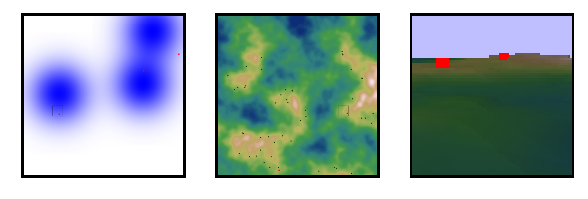
\includegraphics[scale=0.75]{figures/environments.pdf}}
%\logo{
\includegraphics[height=0.5cm]{../report/figures/liu_primary_black_en.pdf}}

\begin{document}

\begin{frame}
    \titlepage
\end{frame}

\begin{frame}
    \frametitle{Outline}
    \tableofcontents
\end{frame}

\chapter{Introduction}
\label{cha:introduction}

In this thesis project, the problem of searching for targets in unknown but familiar environments is addressed.
This chapter presents the motivation behind the project, the research questions that are addressed, and the delimitations. 

% there is extensive research in visual search.
% can a learning agent exhibit these behaviours?
% can also downplay visual aspect
% specify actions properly: how do they transform view, and what does the trigger correspond to? 

\section{Motivation}
\label{sec:motivation}

% This is where the studied problem is described from a general
% point of view and put in a context which makes it clear that
% it is interesting and well worth studying. The aim is to make
% the reader interested in the work and create an urge to
% continue reading.

The ability to visually search for targets in an environment is crucial to many parts of our daily lives.
We are constantly looking for things, be it the right book in the bookshelf, a certain keyword in an article or blueberries in the forest.
In many cases, it is important that this search is efficient and fast.
Animals need to quickly identify predators, and drivers need to be able to search for pedestrians crossing the road they are driving on.

While searching for targets is often seemingly effortless to humans, it is a complex process.
How humans and animals search for things has been extensively studied in neuroscience and neurobiology~\cite{eckstein_visual_2011,wolfe_visual_2010,wolfe_guided_2021}.
Applications from automated search and rescue to helping robots mean that it is of great interest to automate visual search.
In the computer vision field, there has been several attempts to mimic the way humans search in machines~\cite{}.
Most attempts focus on fully observable scenes where the target is in view and the task is to localize it (object localization).
However, in many real-world visual search scenarios the field-of-view is limited.
This means that the search process is split into two steps: directing the field of view (covert attention), and locating targets within the view (overt attention).
Much work has been focused on latter, locating targets within the field of view~\cite{}. 

When only a fraction of the environment is visible, where to move the field of view becomes an important decision.
The characteristics of the searched environment can often be used to find targets quicker.
For example, if one is foraging for blueberries it makes sense to search the ground rather than the trees.
Similarly, if one is searching a satellite image for boats it is reasonable to focus on ocean shores.
If you see a railroad track or the wake of a boat you can usually follow it to find a vehicle.
The exact characteristics of the environment need not be constant - forests with blueberries can vary greatly in appearance and boats can be found in all of the seven seas.
In many cases, the environment is familiar in that it has characteristics that are similar to previously seen environments.
Humans are able to generalize in such cases.

Manually creating search algorithms for such tasks is problematic.
The appearance and distribution of targets in an environment varies greatly, and may be subtle.
The visual richness of the environment itself is another problem.
How can you identify useful hints from the environment to guide covert attention?
Manually engineering such a platform seems infeasible.
If one could instead learn the underlying from a limited set of sample environments and generalize to unseen similar environments this problem would be circumvented.

% we want a system that can
% - work in familiar environments
% - learns effective scanning patterns
% - in the best case better than exhaustive
% - integrates history (features, location, etc)

% - train: show the agent some samples of previous objects and their locations
% - test: the agent finds them in a short time

\section{Aim}
\label{sec:aim}

% What is the underlying purpose of the thesis project?

This work tries to address these issues, focusing on strategic scans of larger environments where the field of view is small relative to the environment.
This is a problem that has been less studied in the literature than visual search in smaller environments.
There are other factors that become increasingly important. The field-of-view of the observer is often limited, and she has to move it efficiently to find the target.

% what will be done
The aim of this thesis is to implement and evaluate an autonomous agent that intelligently searches its environment for targets.
The agent should learn common characteristics of environments and utilize this knowledge to search for targets in new environments more effectively.
Furthermore, the agent should be able to generalize to unseen environments drawn from the same distribution as the ones it has seen previously.

% how it will be done
A specific instance of the visual search problem is considered, where the environment is searched by a pan-tilt camera fixed in place.
The camera has a limited view of the environent.
Automating this task is of interest for multiple reasons.
Manually controlling a camera may be costly, and the performance of a human operator may be suboptimal.
Crucial to the problem is generalization.

\section{Research questions}
\label{sec:research-questions}

% This is where the research questions are described.
% Formulate these as explicit questions, terminated with a
% question mark. A report will usually contain several different
% research questions that are somehow thematically connected.
% There are usually 2-4 questions in total.
% 
% Examples of common types of research questions (simplified
% and generalized):
% 
% \begin{enumerate}
% \item How does technique X affect the possibility of achieving the
%   effect Y?
% 
% \item How can a system (or a solution) for X be realized so
%   that the effect Y is achieved?
% 
% \item What are the alternatives to
%   achieving X, and which alternative gives the best effect considering
%   Y and Z? (This research question is normally broken down in to 2
%   separate questions.)
% 
% \end{enumerate}
% 
% 
% Observe that a very specific research question almost always
% leads to a better thesis report than a general research question
% (it is simply much more difficult to make something good
% from a general research question.)
% 
% The best way to achieve a really good and specific research
% question is to conduct a thorough literature review and get
% familiarized with related research and practice. This leads to
% ideas and terminology which allows one to express oneself
% with precision and also have something valuable to say in the
% discussion chapter. And once a detailed research question
% has been specified, it is much easier to establish a suitable
% method and thus carry out the actual thesis work much faster
% than when starting with a fairly general research question. In
% the end, it usually pays off to spend some extra time in the
% beginning working on the literature review. The thesis
% supervisor can be of assistance in deciding when the research
% question is sufficiently specific and well-grounded in related
% research.

This thesis will address the following questions:

\begin{enumerate}
  \item How can a learning agent that does efficient visual search in familiar environments be implemented?
  \item How well does the learning agent generalize to unseen but familiar environments?
  \item How does the learning agent compare to an exhaustive search of the environment, frontier-based algorithm, and a human searcher?
  %\item How does the learning agent compare to common non-learning methods?
  %\item How can a simulator that tests the ability of an agent to solve the presented problem be implemented?
  %\item How does memory affect the agent's ability to search an environment?
\end{enumerate}

\section{Delimitations}
\label{sec:delimitations}

% This is where the main delimitations are described. For
% example, this could be that one has focused the study on a
% specific application domain or target user group. In the
% normal case, the delimitations need not be justified.

This thesis will be focused on the behavioral aspects of the presented problem.
To train and test agents, a simplified environment will be used. 
This will test the desired characteristics of the agent as presented above, but will not simulate realistic environments.
For simplicity, we assume that the environment is static. % explain
We also focus on the search process and not the detection, and therefore targets will be easy to detect once visible.

% Having a variable number of targets becomes problematic: an exhaustive search of the environment is necessary for the agent to know for certain if it is done.

\chapter{Theory}
\label{cha:theory}

% ~10p

% The main purpose of this chapter is to make it obvious for
% the reader that the report authors have made an effort to read
% up on related research and other information of relevance for
% the research questions. It is a question of trust. Can I as a
% reader rely on what the authors are saying? If it is obvious
% that the authors know the topic area well and clearly present
% their lessons learned, it raises the perceived quality of the
% entire report.
% 
% After having read the theory chapter it shall be obvious for          <--
% the reader that the research questions are both well                  <--
% formulated and relevant.                                              <--
% 
% The chapter must contain theory of use for the intended
% study, both in terms of technique and method. If a final thesis
% project is about the development of a new search engine for
% a certain application domain, the theory must bring up related
% work on search algorithms and related techniques, but also
% methods for evaluating search engines, including
% performance measures such as precision, accuracy and
% recall.
% 
% The chapter shall be structured thematically, not per author.
% A good approach to making a review of scientific literature
% is to use \emph{Google Scholar} (which also has the useful function
% \emph{Cite}). By iterating between searching for articles and reading
% abstracts to find new terms to guide further searches, it is
% fairly straight forward to locate good and relevant
% information, such as \cite{test}.
% 
% Having found a relevant article one can use the function for
% viewing other articles that have cited this particular article,
% and also go through the article’s own reference list. Among
% these articles on can often find other interesting articles and
% thus proceed further.
% 
% It can also be a good idea to consider which sources seem
% most relevant for the problem area at hand. Are there any
% special conference or journal that often occurs one can search
% in more detail in lists of published articles from these venues
% in particular. One can also search for the web sites of
% important authors and investigate what they have published
% in general.
% 
% This chapter is called either \emph{Theory, Related Work}, or
% \emph{Related Research}. Check with your supervisor.

This chapter introduces background and related work.

% background: neuroscience, framework
% related work: practical aspects, reinforcement learning

\section{Background}

% covert/overt: reactionary/requires memory! 

\subsection{Active Vision}

% Marr?
~\cite{zeng_survey_2020}
Much of past and present research in machine perception involves a passive observer.
Images are passively sampled and perceived.
Animal perception, however, is active.
We do not only see things, but look for them.
One might ask why this is the case, if there is any advantage that an active observer has over a passive one.
Aloimonos and Weiss~\cite{aloimonos_active_1988} introduce the paradigm called \textit{active vision}, and prove that an active observer can solve several basic vision problems in a more efficient way than a passive one.

Bajcsy~\cite{bajcsy_1988} defines active vision, and perception in general, as a problem of intelligent data acquisition.
An active observer needs to define and measure parameters and errors from its scene and feed then back to control the data acquisition process.
Bajscy states that one of the difficulties of this problem is that they are scene and context dependent.
A thorough understanding of the data acquisition parameters and the goal of the visual processing is needed.
One view lacks information that may be present with multiple views.
Multiple views also add the time dimension into the problem.

In a re-visitation of active perception, Bajcsy, Aloimonos and Tsotsos~\cite{bajcsy_aloimonos_tsotsos_2018} stress that despite recent successes in robotics, artificial intelligence and computer vision, an intelligent agent must include active perception:

\begin{quote}
    An agent is an active perceiver if it knows why it wishes to sense, and then chooses what to perceive, and determines how, when and where to achieve that perception
\end{quote}~\cite{bajcsy_aloimonos_tsotsos_2018}

% see conclusion in that paper:
% - mirror neurons, same system responsible for generating and interpreting actions at a high level 

\cite{chen_activevisionsurvey_2011}

\subsection{Visual Search}
\label{sec:visualsearch}

% todo: should maybe remove the psychology and keep that in introduction only

The perceptual task of searching for something in a visual environment is usually referred to as \textit{visual search}.
The searched object or feature is the \textit{target}, and the other objects or features in the environment are the \textit{distractors}.
This task has been studied extensively in psychology and neuroscience.
% the reason for introducing this is to be able to use the same terminology later

Wolfe~\cite{wolfe_guided_2021} describes a model of visual search

% general things
% - foveated vision
% - covert and overt attention

Eckstein~\cite{eckstein_visual_2011} reviews efforts from various subfields and identifies a set of mechanisms used to achieve efficient visual search.
Knowledge about the target, distractor, background statistical properties, location probabilities, contextual cues, rewards and target prevalence are all identified as useful.
This is motivated with evidence from psychology as well as neural correlates.

Visual search is not always instant, and can in fact often be slow.
This is in part due to processing: our visual system cannot process the entire visual field and 

% saliency, center-surround organization
% covert attention and eye movement

Wolfe and Horowitz~\cite{wolfe_horowitz_2017} identify and measure a set of factors that guide attention in visual search.
One of these is bottom-up guidance, in which some visual properties of the scene draw more attention than others.
Another is top-down guidance, which is user driven and directed to objects with known features of desired targets.
Scene guidance is also identified, in which attributes of the scene guide attention to areas likely to contain targets. 

These works ground the task considered in this project in psychology.

% can we build a system that exhibits all of these?

\subsection{Visual Attention}

\dots

\subsection{Reinforcement Learning}

% {arulkumaran_survey_2017} also gives a good introduction to algorithms

% https://www.davidsilver.uk/wp-content/uploads/2020/03/intro_RL.pdf
% https://spinningup.openai.com/en/latest/spinningup/rl_intro2.html
% https://sites.ualberta.ca/~szepesva/rlbook.html

Reinforcement learning (RL)~\cite{sutton_reinforcement_2018} is a subfield of machine learning concerned with learning from interaction how to achieve a goal.
This section introduces the fundamental concepts of RL.

\subsubsection{Partially Observable Markov Decision Processes}

The problem of learning from interaction to achieve some goal is often framed as a Markov decision process (MDP).
A learning \textit{agent} interacts continually with its \textit{environment}.
The agent takes the \textit{state} of the environment as input, and select an \textit{action} to take.
This action updates the state of the environment and gives the agent a scalar \textit{reward}.
It is assumed that the next state and reward depend only on the previous state and the action taken.
This is referred to as the \textit{Markov} property.~\cite{kaelbling_pomdp_1998}

In an MDP, the agent can perceive the state of the environment with full certainty.
For many problems, including the one we consider here, this is not the case.
The agent can only perceive a partial representation of the environment's state.
Such a process is referred to as a partially observable Markov decision process (POMDP).
A POMDP is formally defined as a 7-tuple \(\left\langle \mathcal{S}, \mathcal{A}, \mathcal{T}, \mathcal{R}, \Omega, \mathcal{O}, \gamma \right\rangle\), where

\begin{itemize}
    \item \(\mathcal{S}\) is a finite set of states,
    \item \(\mathcal{A}\) is a finite set of actions,
    \item \(\mathcal{T}: \mathcal{S} \times \mathcal{A} \rightarrow \Pi(\mathcal{S})\) is a state-transition function,
    \item \(\mathcal{R}: \mathcal{S} \times \mathcal{A} \rightarrow \mathbb{R}\) is a reward function,
    \item \(\Omega\) is a finite set of observations,
    \item \(\mathcal{O}: \mathcal{S} \times \mathcal{A} \rightarrow \Pi(\Omega)\) is an observation function, and
    \item \(\gamma \in [0, 1]\) is a discount factor.
\end{itemize}

Assume that the environment is in state \(s_t \in \mathcal{S}\), and the agent selects action \(a_t \in \mathcal{A}\).
Then, \(T(s_t, a_t, s_{t+1})\) is the probability of ending in state \(s_{t+1}\) and \(r_t = R(s_t, a_t)\) is the expected reward gained by the agent.
The agent also receives an observation \(o_t \in \Omega\) with probability \(\mathcal{O}(s_{t+1}, a_t, o_t)\).~\cite{kaelbling_pomdp_1998}
Figure \ref{fig:pomdp} illustrates the interaction between agent and environment.

\begin{figure}
    \centering
    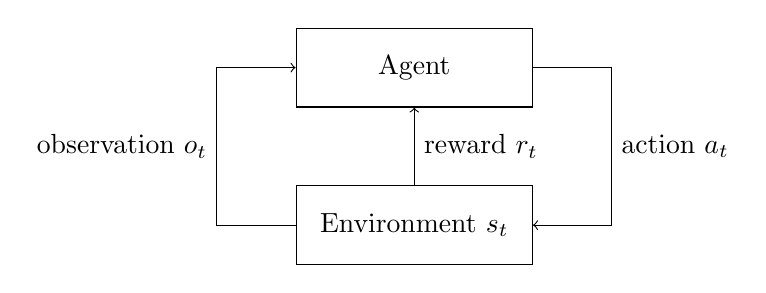
\begin{tikzpicture}[node distance=2cm]
    \tikzstyle{block} = [rectangle,minimum width=3cm,minimum height=1cm,text centered,draw=black,fill=white]
    \node (agent)[block]{Agent};
    \node (environment)[block,below of=agent]{Environment \(s_t\)};
    \draw [->] (agent.east) -- ++(1cm,0) -- node [anchor=west]{action \(a_t\)} ++(0,-2cm) -- (environment.east);
    \draw [->] (environment.north) -- node [anchor=west]{reward \(r_t\)} (agent.south);
    \draw [->] (environment.west) -- ++(-1cm,0) -- node [anchor=east]{observation \(o_t\)} ++(0,+2cm) -- (agent.west);
\end{tikzpicture}
    \label{fig:pomdp}
    \caption[Partially observable Markov decision process]{Partially observable Markov decision process.}
\end{figure}

The agent and environment interact over a sequence of discrete time steps \(t = 0, 1, \dots, T\), giving rise to an \textit{episode} of length \(T\).
At each time step \(t\), the goal of the agent is to select the action that maximizes the expected \textit{discounted return}:

\[ 
    \mathbb{E} \left[ \sum_{k=0}^T \gamma^{k-t-1} r_k \right]
\]

Since the agent receives partial observations of the environment's state, it has to act under uncertainty.
Planning in a POMDP is undecidable, and solving them is often computationally intractable.
Approximate solutions are more common, where the agent usually maintains an internal \textit{belief state}~\cite{kaelbling_pomdp_1998} which is acts on.
The belief state summarizes the agent's previous experience and is therefore dependent on the full \textit{history} of actions and observations.
It does not need to summarize the whole history, but generally only the information that helps the agent maximize the expected reward.
From here on we will use the belief state and the environment state \(s\) interchangeably. 
% Sutton page 467 is better, contains latent state assumption


\subsubsection{Policies and Value Functions}
\label{sec:policy-value}

The behavior of the agent is described by its \textit{policy}.
A policy \(\pi\) is a mapping from perceived environment states to actions.
Policies are often stochastic and specify probabilities for each action, with \(\pi(a|s)\) denoting the probability of taking action \(a\) in state \(s\).~\cite{sutton_reinforcement_2018}

Most RL solutions methods also approximate a \textit{value function}.
A value function \(v_\pi\) estimates how good it is to be in a state.
The value function \(v_\pi(s)\) is the expected (discounted) return when starting at state \(s\) and following policy \(\pi\) until the end of the episode.
There are two common alternative value functions:
The \textit{quality function} \(q_\pi(s,a)\) gives the value of state \(s\) under policy \(\pi\) where \(a\) is the first action taken.
Given a quality function, \textit{action-value} methods choose the action greedily at every state as \(arg\,max q_\pi(s, a)\).
The \textit{advantage function} \(a_\pi(s, a)\) instead represents the relative advantage of actions, \(a_\pi = q_\pi - v_\pi\).~\cite{sutton_reinforcement_2018}

For problems with large state and action spaces, it is common to represent value functions with \textit{function approximation}.
In such cases, it is common to encounter states that have never been encountered before.
This makes it important that the estimated value function can generalize from seen to unseen states.
With examples from the true value function, an approximation can be made with supervised learning methods.
We write \(\hat{v}(s,\mathbf{w}) \approx v_\pi(s)\) for the approximate value of state \(s\) with some weight vector \(\mathbf{w} \in \mathbb{R}^d\).~\cite{sutton_reinforcement_2018}

An alternative to action-value methods is to approximate the policy itself.
\textit{Policy gradient methods}~\cite{sutton_policygrad_1999} learn a parametrized policy that select actions without a value function.
We denote a parametrized policy as \(\pi(a|s,\boldsymbol{\theta})\) with \(\boldsymbol{\theta} \in \mathbb{R}^{d^\prime}\) as the parameters to the policy.
The policy parameters are usually learned based on the gradient of some performance measure \(J(\boldsymbol{\theta})\).
As long as \(\pi(a|s,\boldsymbol{\theta})\) is differentiable with respect to its parameters, the parameters can be updated with \textit{gradient ascent} in \(J\):

\[
    \boldsymbol{\theta}_{t+1} = \boldsymbol{\theta}_t + \alpha \hat{\nabla J(\boldsymbol{\theta}_t)}) 
\]

Advantages of policy parametrization over action-value methods include stronger convergence guarantees~\cite{sutton_policygrad_1999} and more flexibility in parametrization~\cite{sutton_reinforcement_2018}. In practice, value functions are often still used to learn the policy parameter, but they are not needed for action selection.
Such methods are called \textit{actor-critic} methods, with actor referring to the learned policy and critic referring to the learned value function.
In these cases, there might also be some overlap between the weights \(\mathbf{w}\) of the value function estimate and \(\boldsymbol{\theta}\) of the policy estimate. 

Function approximation includes important aspects of partial observability.
If there is a state variable that is not observable,
then the parametrization can be chosen such that the approximate value does not depend on that state variable.
Because of this, function approximation is applicable to the partially observable case.

% https://www.quora.com/What-are-the-benefits-of-actor-critic-framework-in-reinforcement-learning

% We might imagine an artificial neural network (ANN) in which the last layer is split into multiple parts, or heads, each working on a di↵erent task. One head might produce the approximate value function for the main task (with reward as its cumulant) whereas the others would produce solutions to various auxiliary tasks. All heads could propagate errors by stochastic gradient descent into the same body—the shared preceding part of the network—which would then try to form representations, in its next-to-last layer, to support all the heads. Researchers have experimented with auxiliary tasks such as predicting change in pixels, predicting the next time step’s reward, and predicting the distribution of the return. In many cases this approach has been shown to greatly accelerate learning on the main task (Jaderberg et al., 2017). Multiple predictions have similarly been repeatedly proposed as a way of directing the construction of state estimates (see Section 17.3). (Sutton)

\subsubsection{Challenges in Reinforcement Learning}

% we can illustrate the challenges in terms of our problem

One of the challenges that arises in reinforcement learning is the exploration-exploitation trade-off.
An RL agent should \textit{exploit} knowledge gained from previous experiences and prefer actions that has yielded reward in the past.
It should also \textit{explore} in order to learn better actions to take in the future.
Agents that fail to both exploit and explore will lead to failure at the task.
%Furthermore, striking a good balance between the two is non-trivial, and often requires care.~\cite{sutton}

Another challenge is the design of reward signals.
For some tasks, like certain video games, the objective is simply to maximize the score obtained.
In this case there is an inherent reward signal and the agent achieves its task simply by maximizing this inherent signal.
Other times, we have a task we want the agent to solve and have to design a reward signal around that task.
Designing rewards is not straight-forward and can often have unintended effects~\cite{sutton_reinforcement_2018}.
Special care has to be taken to ensure that the reward encourages the desired behavior.

Here, the problem of \textit{sparse rewards} also comes into play.
The agent has to be reward frequently enough to allow it to achieve its goal once.
Often it has to incentivize it to achieve its goal efficiently, with multiple different starting conditions.
If rewards are too sparse, the agent may explore aimlessly and take too long to find achieve its goal.
In such cases, it can be effective to modify the reward to give the agent hints along the way.
If the received reward is temporally distant from the action that caused it, the agent may have difficulty connecting the two.
This is known as the \textit{credit assignment problem}~\cite{minsky_cap_1961}.

In practice, rewards are often designed through trial-and-error.
Several iterations of a reward signal are tried until one yields expected and sufficient results.

% Reward shaping is a technique to tackle\dots~\cite{mataric_shaping_1994}
% https://ai.stackexchange.com/questions/12908/what-is-the-credit-assignment-problem
% https://medium.com/@m.k.daaboul/dealing-with-sparse-reward-environments-38c0489c844d
% reward shaping

\subsection{Deep Learning}

Deep learning is a family of techniques in which hypothesis are represented as computation graphs with tunable weights.
The computation graphs are inspired by biological neurons in the brain and are referred to as \textit{neural networks}.
Deep neural networks consist of \textit{nodes} arranged in \textit{layers}: one input layer, zero or more hidden layers and one output layer.
Each layer receives an input \textit{representation}~\cite{bengio_representation_2014} from the previous layer and outputs a transformed representation to the next layer.
Given some input, a neural network optimizes its output representation with regard to some criterion.
Usually, a loss function \(\mathcal{L}\) is minimized by updating the weights \(\mathbf{w}\) of the network with some variant of \textit{gradient descent} with learning rate \(\alpha\):

\begin{equation}
    \mathbf{w} \leftarrow \mathbf{w} - \alpha \nabla_\mathbf{w} \mathcal{L}(\mathbf{w}) 
\end{equation}

The only requirement on the functions computed by each node is that it is differentiable.
As long as this holds, layers can be stacked arbitrarily and the gradients can be computed with the chain rule.
This way, errors in the output can be passed back through the network (\textit{back-propagation}) and used to update the weights.~\cite{russell_artificial_2021,goodfellow_deep_2016}

The architecture of a neural network imposes some bias onto the learning that its expected to be useful for generalizing to unseen samples.
We now describe three neural network architectures that will be used in this work.

\subsubsection{Feedforward Neural Network}

A feed-forward neural network, also known as a multi-layer perceptron (MLP)~\cite{goodfellow_deep_2016}, only has connections in one direction.
Each node in the network receives inputs from its predecessors and outputs the result of a function of those inputs.
The output \(y\) of each node is usually computed by taking the weighted sum of its inputs \(x\) and applying some non-linear function

\begin{equation}
    y_j = g_j(\mathbf{w}_j^T \mathbf{x}),
\end{equation}

where \(y_j\) is the output of node \(j\), \(g_j\) is a non-linear \textit{activation function}, \(\mathbf{w}_j\) is the vector of weights leading into node \(j\), and \(\mathbf{x}\) is the vector of inputs to the node.
By convention, each layer also has some \textit{bias} that allows the total weighted input to \(g_j\) to be non-zero even when the outputs from the previous layer are zero.
The bias is included as an extra input \(x_0\) fixed to 1, and an extra tunable weight \(w_{0,j}\).
The non-linearity ensures that a network with at least two layers can approximate any continuous function.~\cite{russell_artificial_2021}

\subsubsection{Convolutional Neural Network}

Convolutional neural networks (CNNs) contain spatially local connections.
They have patterns of weights, called \textit{kernels}, that are replicated across units in each layer.
With some input vector \(\mathbf{x}\) of size \(n\) and a vector kernel \(\mathbf{k}\) of size \(l\), the (discrete) convolution operation \(\mathbf{z} = \mathbf{x} \ast \mathbf{k}\) is defined as

\begin{equation}
    z_i = \sum_{j=1}^l k_j x_{j+1-\frac{l+1}{s}},
\end{equation}

where \(s\) is the \textit{stride}.
This operations can be generalized up to more than one dimension, such as 2 dimensions for images and 3 dimensions for volumes.
With multiple input channels, kernels are stacked into a \textit{filter}.
The outputs of each kernel are then summed over, giving one output channel per filter.

There are several advantages to using CNNs for structured input data where neighboring values are correlated.
Kernels are smaller than the input, which means that fewer parameters have to be stored.
These \textit{sparse interactions} give CNNs reduced memory requirements,
as well as improved statistical and computational efficiency.

Furthermore, the same parameters are also used for more than one function in the CNN. \textit{Parameter sharing} across input locations mean that layers in a CNN have \textit{equivariance} to translation. 
The output of one kernel is the same regardless of the input location.
This property of CNNs is useful for images where similar features may be useful regardless of their location in the input.~\cite{goodfellow_deep_2016}

%A common augmentation to deep CNNs is \textit{residual networks}.

\subsubsection{Recurrent Neural Network}

Recurrent neural networks (RNNs) extend feed-forward networks by allowing cycles in the computation graph.
Each cycle has a delay so that some \textit{hidden state} from the previous computation is used as input to the current computation.
A recurrent layer with input \(\mathbf{x}_t\), output \(\mathbf{y}_t\) and hidden state \(\mathbf{z}_t\) is defined by

\begin{align}
    \begin{split}
        \mathbf{z}_t &= f_\mathbf{w}(\mathbf{z}_{t-1}, \mathbf{x}_t) \\
        \mathbf{y}_t &= g_y(\mathbf{W}_{z,y}, \mathbf{z}_t),
    \end{split}
\end{align}

where \(f_\mathbf{w}\) is the update process for the hidden state and \(g_y\) is the activation function for the hidden layer.
This model can be turned into a feed-forward network over a sequence of input vectors \(\mathbf{x}_1, \dots \mathbf{x}_T\) and observed outputs \(\mathbf{y}_1, \dots, \mathbf{y}_T\) by \textit{unrolling} it for \(T\) steps. The weights are shared across all time steps. This means that RNNs can operate on inputs of arbitrary lengths.
The hidden state is used as a summary of all previous items in the sequence.
Thus, RNNs make a Markov assumption.~\cite{russell_artificial_2021}

In practice, conventional RNNs struggle with learning long-term dependencies.
During back-propagation, gradients can tend to zero for long sequences, something known as the vanishing gradient problem~\cite{goodfellow_deep_2016}.
An architecture that addresses this issue is long short-term memory (LSTM)~\cite{hochreiter_schmidhuber_lstm_1997}.
LSTMs include a \textit{memory cell} \(c\) in the hidden state that is copied from time step to time step, and three soft \textit{gating units} that govern the information flow in the hidden state update process \(f\). This makes LSTMs particularly useful for learning over long sequences.

\section{Related Work}

To our knowledge, there is no work that considers the exact problem we are looking at.
In this section, we present work that considers similar tasks.

\subsection{Deep Reinforcement Learning}

% Mnih et al., Atari, DQN

As mentioned in Section~\ref{sec:policy-value}, policies and value functions are often approximated.
Neural networks have good properties for function approximation and have been used for RL with success.
One early example is TD-Gammon~\cite{tesauro1995tdgammon}, a neural network trained with RL that reached expert Backgammon performance in 1995.

More recently, the successes of deep learning have bled over into the field of RL.
In 2015, Mnih et al.~\cite{mnih_human_2015} extend \cite{mnih_atari_2013} and introduce DQN, which combines deep neural networks with RL and gives birth to the field of deep reinforcement learning (deep RL).
DQN approximates the quality function \(q(s, a)\) with a CNN, and select actions greedily using only visual input.
To incorporate some memory, images from the 4 previous time steps are stacked and used as input to the neural network.
The input is fed through three convolutional layers:
32 \(8\times8\) filters with stride 4,
followed by 64 \(4\times4\) filters with stride 2,
followed by 64 filters of size \(32\times32\) with stride 1.
Between each convolutional layer is a ReLU activation function.
Then, there is a hidden fully connected layer with a ReLU activation function.
The output layer has one output for each valid action.
% replay buffer
% instability
% follow up works
% architecture
%\cite{arulkumaran_survey_2017}

The DQN architecture sparked great interest and several modifications.
Hausknecht and Stone~\cite{hausknecht_stone_2017} investigate the effects of adding a recurrent step to DQN in order to tackle POMDPs.
They use the same convolutional network as \cite{mnih_human_2015}, but only use the most recent frame as input and replace the hidden layer with a recurrent LSTM.
It is found that the agent is able to integrate information over time and achieves comparable performance to the original DQN agent.

\subsection{Proximal Policy Optimization}

% ~\cite{zeng_survey_2020} has a concise overview of algorithms

Proximal policy optimization algorithms\dots~\cite{schulman_ppo_2017}.
\todo{Expand on algorithm, advantages, practicalities, etc.}

\begin{algorithm}
    \caption{Proximal Policy Optimization}
    \begin{algorithmic}
        \For{\(\text{iteration} = 1,2,\dots\)}
            \For{\(\text{actor} = 1,2,\dots,N\)}
                \State \(\text{Run policy } \pi_{\theta_\text{old}} \text{ for } T \text{ time steps}\)
                \State \(\text{Compute advantage estimates } \hat{A}_1, \dots \hat{A}_T\)
            \EndFor
            \State \(\text{Optimize surrogate } L \text{ wrt } \theta, \text{ with } K \text{ epochs and mini-batch size } M \leq NT\)
            \State \(\theta_{\text{old}} \leftarrow \theta\)
        \EndFor
    \end{algorithmic}
\end{algorithm}

\subsection{Active Object Detection}

% active object detection

In computer vision, \textit{object detection} is the task of detecting semantic objects of a certain class in images.
Detecting an object entails \textit{recognizing} that it is present in an image, and \textit{localizing} it by determining its bounding box.
State of the art object detection use deep learning techniques and usually involve a deep convolutional architecture~\cite{zhao_objectdetection_2019}.
Object detectors usually use region proposal networks that consider the whole image and return a set of bounding box candidates.
The object recognizer is then run on each region proposal.

Although we do not focus on difficult recognition problems in this work, the task we consider bears resemblance to object localization.
The difference is that images in object detection are passively sampled - they are drawn from some distribution and all are independent.
Furthermore, the whole scene that is searched for objects is visible in the image.
In \textit{active object detection}, the analyzed images are instead chosen so as to help the detector perform its task better.

Caicedo and Lazebnik~\cite{caicedo_active_2015} propose to use deep reinforcement learning for active object localization in images where the object to be localized is fully visible.
An agent is trained to successively improve a bounding box using translating and scaling transformations.
They use a reward signal that is proportional to how well the current box covers the target object.
An action that improves the region is rewarded with +1, and given a punishment of -1 otherwise.
They find that this reward communicates more clearly which transformations keep the object inside the box and which take the box away from the target.
When there is no action that improves the bounding box, the agent may select a trigger action (which would be the only action that does not give a negative reward) which resets the box.
This way the agent may select additional bounding boxes.
Each trigger modifies the environment by marking it so that the agent may learn to not select the same region twice. % inhibition-of-return mechanism, widely used in visual attention models ~\cite{itti_koch_2001}

A similar work by Ghesu et al.~\cite{ghesu_artificial_2016} present an agent for anatomical landmark detection trained with DRL.
Different from \cite{caicedo_active_2015} is that the entire scene is not visible at once.
The agent sees a limited region of interest in an image, with its center representing the current position of the agent.
The actions available to the agent translate the view up, down, left and right.
A reward is given to the agent that is equal to the supervised relative distance-change to the landmark after each action.
Three datasets of 891 anatomical images are used.
The agent starts at random positions in the image close to the target landmark and is tasked with moving to the target location.
While achieving strong results (90\% success rate), the scenes and targets are all drawn from a distribution with low variance.
Most real-world search tasks exhibit larger variance than a population of anatomical images of the human body.

% ghesu_multiscale_2019

Chen and Gupta~\cite{chen_memory_2017} use a spatial memory for context reasoning in object detection.
They argue that object detection systems require memory to perform well,
Furthermore, they pose that this memory should capture the spatial layout of the scene in order to model object-object relationships.
A spatial memory network is proposed, which remembers features and locations of past detections in an image and uses this to improve future ones.
A CNN is used to extract features from the memory and used together with the original image as input to a standard region proposal network.
The approach gives a small improvement over the standalone region proposal network.

\subsection{Visual Attention}

Visual attention in humans is often split into two phases usually split into two phases

~\cite{itti_koch_2001}


% this article is very good!
% note: reinforcement learning part, soft and hard attention
% https://shairozsohail.medium.com/a-survey-of-visual-attention-mechanisms-in-deep-learning-1043eb25f343

% "Looking through a foggy pane of glass represents soft attention, where the entire image is still being “seen”, but certain areas are being attended to more. Whereas the binoculars represent hard attention, where we are only seeing a subset of the image, hopefully the part most relevant to our task. The Recurrent Models of Visual Attention paper from above represents hard attention. The key thing to take away is that there are explicit trade-offs between these attention types: hard attention requires significantly less computation and memory (as the entire image is not being stored or operated over usually) but cannot be easily trained as the objective is non-differentiable (there is no gradient, pixels are either seen or unseen). Hence it is often trained with methods like REINFORCE. Soft attention on the other hand often requires more memory and computation (often even more then simple convolutional nets) but has a differentiable objective and can be easily trained with standard back propagation methods." <- some good points here

% closely connected with object detection

\cite{minut_mahadevan_2001}

\cite{mnih_attention_2014}

Soft attention (Bahdanau~\cite{bahdanau_attention_2016})\dots

Partially observable processes, such as the one we consider in this work, can be seen as hard attention problems.
By taking actions, the hard attention can be redirected.

\subsection{Coverage Path Planning}

% could be a smaller section in background, under visual search

The problem we consider in this work shares many characteristics with coverage path planning (CPP)~\cite{galceran_carreras_2013}.
CPP is the task of determining a path that passes over all points in an area, and appears as a fundamental part of many real-world problems. 
In the general case, an agent that does not learn to exhaustively search its environment can not be expected to be successful for the visual search task.
The CPP is strongly related to the traveling salesman problem (TSP).
The unrestricted CPP where there are no obstacles (the "lawnmower problem") is in fact proven to be NP-hard~\cite{arkin_lawnmowing_2000}.
In our problem, we do not require complete coverage, but just that certain points (those that contain targets) are visited.
The shape of the environment is known, as the sensor has limited range of movement.
Furthermore, a good agent should also prioritize certain regions which is not part of the CPP task.
Although a CPP agent that is able to recognize targets is not optimal, it is a suitable baseline for the task.
Specifically, the wavefront algorithm~\cite{galceran_carreras_2013} which is suitable for grid-discretized can be used. % some simple approximation

% \cite{krishna_tetromino_2020} -connection to RL

\subsection{Visual Navigation}

The task we consider is perhaps most similar to visual navigation.
Visual navigation is the process of determining a suitable path between a start point and destination point using visual input~\cite{bonin-font_visnav_2008}.
Visual navigation has been studied for use in both autonomous ground vehicles, where obstacles have to be avoided, as well as for unmanned aerial vehicles which typically don't have the problem of avoiding obstacles.

Bonin et al.~\cite{bonin-font_visnav_2008} divide visual navigation in map-building and map-less systems.
They further subdivide map-less navigation systems into optical flow-based systems, appearance-based systems, 

More recently, deep RL has begun making its way into navigation as well~\cite{zeng_survey_2020}.
The difficulty of hand-engineering 

Navigation can be divided into map-building and map-less navigation.
Map-less techniques are reactive, and typically do not need 

Traditionally, visual navigation is divided into indoor navigation and outdoor navigation. Outdoor navigation is subdivided in structured and unstructured environments. Indoor navigation is subdivided in map-building and map-less navigation  

Navigational systems that don't have previous knowledge of their environment have to perceive their environment while navigating through it.
Such systems often build an internal map and thus require some form of memory.



The field is gaining popularity and 

% most involve showing


% Point navigation / Object Navigation




Mnih et al.~\cite{mnih_asynchronous_2016} use a recurrent policy with only RGB images to navigate in a labyrinth.
3D labyrinths are randomly generated, and an agent is tasked with finding objects in them.
The same architecture as in \cite{mnih_human_2015} is used, but with 256 LSTM cells after the final hidden layer.

% https://aihabitat.org/challenge/2020/#task-1-pointnav
% https://aihabitat.org/challenge/2020/#task-2-objectnav
% https://arxiv.org/pdf/1709.06158.pdf
% https://ieeexplore.ieee.org/document/9102361


Mirowski et al.~\cite{mirowski_navigate_2017}...

Henriques and Vedaldi~\cite{henriques_vedaldi_2018} use a spatial memory...

Gupta et al.~\cite{gupta_cognitive_2019} use a latent spatial memory.
The 
They also use a planner that can plan paths given partial information of the environment.
This allows the agent to take appearance of visited locations into account when deciding where to look next.
The RGB observation is fed through an encoder network that\dots
Planning in this fashion s
% has a list of baselines
% among them is an lstm baseline

Dhiman et al.~\cite{dhiman_critical_2019} critically investigate deep RL for navigation.
They ask whether DRL algorithms are inherently able to gather and exploit environmental information for during navigation.
Experimentally, they find that an agent is able to exploit environment information when trained and tested on the same map.
However, when trained and tested on different maps, it cannot do so successfully.
They further find that, with a single decision point whose correct\dots
% could be due to their inductive biases
% the agent does not have access to its location and can therefore not determine its location
% their setup:
% - random maze
% - when agent finds goal, it respawns and the goal is at the same location (+10)
% - smaller rewards scattered in area to incentivize exploration (+1)
% - wall penalty (-2)
% - respawn either static or random
% - randomly textured walls

Chaplot et al.~\cite{chaplot_semantic_2020} build on the idea of an explicit memory by including environment semantics\dots

Zhu et al.~\cite{zhu_target_driven_2016} create a model for target-driven visual navigation in indoor scenes with DRL.
An observer is given a partial image of its scene as well as an image of the target object, and is tasked with navigating to the object n the scene with a minimal number of steps.
The agent moves forwards, backwards, and turns left and right at constant step lengths.
They use a reward signal with a small time penalty to incentivize task completion in few steps.
They compare their approach to random walk and the shortest path and achieve promising results.
This setup is quite similar to the one considered in this report, but the authors make a few assumptions that we do not.
They a set of 32 scenes, each of which contain a fixed number of object instances.
They focus on learning spatial relationships between objects in these specific scenes, and have scene-specific layers to achieve this.
Thus, while they show that they can adapt a trained network to a new scene, their approach is unable to zero-shot generalize to new scenes.

A similar work by Ye et al.~\cite{ye_active_2018} integrates an object recognition module with a deep reinforcement learning based visual navigation module.
They experiment with a set of reward functions and find that constant time penalizing rewards can be problematic and lead to slow convergence.
Their experiments make the same assumptions as \cite{zhu_target_driven} - the scenes and targets used during testing have all been seen during training.

Several works in visual navigation have placed emphasis on memory representations.~\cite{savinov_topmem_2018,oh_minecraft_2016,parisotto_salakhutdinov_2017,chen_memory_2017} % cite more


%
% this is where we briefly discuss the related work
% emphasize the memories, problems in evaluation, generalization
%


\subsection{Memory Architectures}

A recurring theme in the related work above is the use of memory architectures.
In most cases where active sensing is involved, memory is a requirement for good performance.
Works that don't use memory rely on either full observability, like \cite{caicedo_active_2015}, or low variance so that scenes can be remembered, like \cite{ghesu_artificial_2016}.

Simple memory mechanisms, like the frame stacking used in \cite{mnih_human_2015} can model velocity and work well in certain environments where reactive action is sufficient.
Once a task requires integration of features over longer time, more advanced memory is required.
RNNs provide a suitable memory architecture for many such tasks, and is used which success in works like \cite{mnih_attention_2014}, \cite{mnih_asynchronous_2016}, \cite{...}.

% advanced memory, spatial memory, etc.

\begin{enumerate}
    \item Frame stacking
    \item Recurrent networks
    \item Explicit memories~\cite{oh_minecraft_2016,parisotto_salakhutdinov_2017}.
    % oh remembers over the past K frames, parisotto remembers the entire world
    % parisotto tests on 3d environment. if we don't, we should at least discuss it.
\end{enumerate}


Oh et al. ~\cite{oh_minecraft_2016} use a differentiable retrieval memory.

Parisotto and Salakhutdinov~\cite{parisotto_salakhutdinov_2017} propose a structured memory\dots % this one is very interesting

% could have a section for memory mechanisms
% this is detailed in the survey \cite{arulkumaran_survey_2017}
% Taking recurrent processing further, it is possible to add a differentiable memory to the DQN, which allows it to more flexibly process information in its “working memory” [96]. In traditional RNNs, recurrent units are responsible for both performing calculations and storing information. Differentiable memories add large matrices that are purely used for storing information, and can be accessed using differentiable read and write operations, analagously to computer memory. With their key-value-based memory Q-network (MQN), Oh et al. [96] constructed an agent that could solve a simple maze built in Minecraft, where the correct goal in each episode was indicated by a coloured block shown near the start of the maze. The MQN, and especially its more sophisticated variants, significantly outperformed both DQN and DRQN baselines, highlighting the importance of using decoupled memory storage. More recent work, where the memory was given a 2D structure in order to resemble a spatial map, hints at future research where more specialised memory structures will be developed to address specific problems, such as 2D or 3D navigation [98]. Alternatively, differentiable memories can be used as approximate hash tables, allowing DRL algorithms to store and retrieve successful experiences to facilitate rapid learning [105].


Anderson et al.~\cite{anderson_evaluation_2018} emphasize the importance of memory mechanisms that support the construction of rich internal representations environments in navigation agents.
Simple agents that are purely reactive and act on the sensory input at the current time step only work for simple tasks.
Augmentations like recurrent update mechanisms add more potential.
More advanced memory mechanisms can be important for better navigation.
The nature of the internal representation is central to the study of embodied navigation.
% more recommendations are there, are they relevant?
% see citations [12, 13, 22, 23, 27] on memory mechanisms
% \cite{gupta_cognitive_2019}
% 

\subsection{Benchmarking Environments}

\begin{itemize}
    \item What is contained in an environment (represents a Markov Decision Process).
    \item What is a good benchmarking environment
    \item Should list some common environments and explain why they are not satisfactory
    \item Motivate why we create our own (higher variance, agent's can not rely on memorizing environments)
\end{itemize}

\subsection{Inductive Biases, Overfitting and Generalization}

% first introduce the reason why generalization is important
% reality is dynamic
% agents need to be robust to variation
% capability to transfer and adapt to unseen but similar environments
% most current research works on benchmarks that do not test this (MuJoCo, Arcade learning environment)

Kirk et al.~\cite{kirk_survey_2022} survey generalization in deep RL.

% refer to survey
% specifically IID (train_dist = test_dist) and OOD environments (train_dist != test_dist)

While deep neural networks have proved to be effective function approximators for RL, they are also prone to \textit{overfitting}.
High-capacity models trained over a long time may memorize the distribution seen during training rather than general patterns.
While studied in supervised learning, overfitting is generally been neglected in deep RL.
Training and evaluation stages are typically not separated.
Instead, the final return on the training environments is used as a measure of agent performance.

Zhang et al.~\cite{zhang_overfitting_2018} study overfitting and generalization in deep RL.
With experiments, they show that RL agents are capable of memorizing training data, even when completely random.
When the number of training samples exceeds the capacity of the agent, they overfit to them.
When exposed to new but statistically similar environments during testing, test performance could vary significantly despite consistent training performance.
The authors argue that good generalization requires that the \textit{inductive bias} of the algorithms is compatible with the bias of the problems.
The inductive bias refers to a priori algorithmic preferences, like neural network architecture.
When comparing MLPs with CNNs, they find that MLPs tend to be better at fitting the training data are worse at generalizing.
When rewards are spatially invariant, CNNs generalize much better than MLPs.
The authors advocate for carefully designed testing protocols for detecting overfitting.
The effectiveness of stochastic-based evaluation depends on the properties of the task.
Agents could still learn to overfit to random training data. 
For this reason, they recommend isolation of statistically tied training and test sets.

In a similar spirit, Cobbe et al.~\cite{cobbe_generalization_2019} construct distinct training and test sets to measure generalization in RL.
They find that agents can overfit to surprisingly large training sets, and that deep convolutional architectures can improve generalization.
Methods from supervised learning, like L2 regularization, dropout, data augmentation and batch normalization are also shown to aid with generalization.

Many current deep RL agents do not optimize the true objective that they are evaluated against,
but rather a handcrafted objective that incorporates biases to simplify learning.
Stronger biases can lead to faster learning, while weaker biases potentially lead to more general agents.
Hessel et al.~\cite{hessel_inductive_2019} investigate the trade-off between generality and performance from the perspective of inductive biases.
Through experimentation with common reward sculpting techniques, they find that learned solutions are competitive with domain heuristics like handcrafted objectives.
Learned solutions also seem to be better at generalizing to unseen domains.
For this reason, they argue for removing biases determined with domain knowledge in future research.


% what does this mean for "oracle" reward signals, such as supervised improvement in distance? 
% it is essentially reward shaping.
% they introduce human bias into the possible policies.
% the agent may fail to discover optimal policies.
% the problem with our reward is that I am not sure it will lead to minimizing time.
% should run experiments with time penalty and trigger reward again...

% in this spirit
Cobbe et al.~\cite{cobbe_procgen_2020} introduce a benchmark for sample efficiency and generalization in RL.
They make use of procedural generalization to decide many parameters of the initial state of the environment.
This forces agents to learn policies that are robust variation and avoid overfitting.
To evaluate sample efficiency of agents in the benchmark, they train and test on the full distribution of states.
To evaluate generalization, they fix the number of training samples and then test on held out levels.
When an episode ends, a new sample is drawn from the training set.
Agents may train for arbitrarily many time steps.
The number of training samples required to generalize is dependent on the particulars and difficulty of the environment.
The authors choose the training set size to be near the region when generalization begins to take effect.
Empirically they find that larger model architectures improve both sample efficiency and generalization.
Agents strongly overfit to small training sets and need many samples to generalize.
Interestingly, training performance improves as the training set grows past a certain threshold.
The authors attribute this to the implicit curriculum of the distribution of levels.

\subsection{Evaluation of Agents}

A problem in state-of-the art RL is reproducibility.
There is often non-determinism, both in the methods and environments used.
Furthermore, many methods have intrinsic variance which can make published results difficult to interpret.
This has meant that reproducing state-of-the-art deep RL results is difficult.

Henderson et al.~\cite{henderson_matters_2018} discuss this problem from multiple perspectives.
Through experimental analysis, they show that:

\begin{itemize}
    \item In policy gradient methods, hyperparameters and the choice of network architecture for policy and value function approximation can affect performance significantly.
    They find that ReLU activations tend to perform best across environments and algorithms.
    For PPO, the use of large networks may require changing other hyperparameters like learning rate.
    \item Rescaling rewards can have a large effect, although it is difficult to predict how.
    \item Variance between random seeds in stochastic environments affects performance of algorithms, and give learning curves that do not fall within the same distribution.
    This suggests that selecting the top \(N\) trials or average over a small number of trials \(N\) can be misleading. They suggest to compare performance over many different random seeds.
    \item For certain environments, learning curves can indicate successful optimization but the learned behavior may not be satisfactory.
    It is therefore important to not only show returns, but also demonstrations of the learned policy in action.
    \item Implementation differences that are not reflected in publications can have a dramatic impact on performance.
    It is therefore necessary to enumerate implementation details and package code bases with publications.
    Performance of baseline experiments should also match original baseline publication code.
\end{itemize}

Due to the unstable nature of RL algorithms, it is often inadequate to just report average return.
\cite{henderson_matters_2018} propose to include confidence intervals when reporting results.
Confidence bounds with sample bootstrapping is used to show that PPO is among the more stable algorithms.
Finally, \cite{henderson_matters_2018} make the point that more emphasis should be placed on applying RL algorithms to real-world tasks.
Benchmarks environments like ALE~\cite{arcade} often have no clear winner.
It could be more useful to propose a set of tasks that an algorithm could be used for than to show performance on fictional tasks.

A similar work by Agarwal et al.~\cite{agarwal_rlliable_2022} criticizes the heavy use of point estimates of aggregate performance.
They show that conclusions drawn from point estimates can be very different from those drawn from more thorough statistical analysis. 
The popularity of more challenging benchmarks has lead to longer training times.
This has made it less feasible to measure performance over many training runs,
which in turn has led to a shift to only evaluating a small number of runs per task.
Like \cite{henderson_matters_2018}, they advocate for the use  of performance metrics that take uncertainty in results into account.
They propose the following set of metrics that better reflect performance across a handful of runs:

\begin{itemize}
    \item Uncertainty in aggregate performance should be reported through interval estimates via stratified bootstrap confidence intervals.
    \item Variability in performance across tasks should be reported through performance profiles (score distributions).
    \item Aggregate metrics for summarizing performance across tasks should be reported through interquartile mean (IQM) across all runs.
\end{itemize}

Anderson et al.~\cite{anderson_evaluation_2018} discuss problem statements and evaluation measures for embodied navigation agents, and make a set of recommendations.
A navigation agent should be equipped with a special action that indicates that it has concluded the episode.
The agent should be evaluated at the time this action is made, and not at some more favorable time step. % implicitly the trigger action for us, since we have multiple targets
Proximity to a goal should be measured using geodesic distance, the shortest distance in the environment. % Manhattan in 2D?
They recommend success weighted by (normalized inverse) path length (SPL) as the primary measure of navigation performance.
With \(N\) test episodes, SPL is computed as 

\begin{equation}
    \frac{1}{N} \sum_{i=1}^N S_i \frac{l_i}{\max(p_i, l_i)}
\end{equation}

% if we adopt SPL, we should note that the optimal path is not realistic for this problem

where \(S_i\) is a binary indicator of success,
\(l_i\) is the shortest path distance from the agent's starting position to the goal,
and \(p_i\) is the length of the path actually taken in the episode.
If 50\% of test episode are successful and the agent takes the optimal path in all of them, its SPL is 0.5.
By measuring SPL of human subjects, what is a good score can be calibrated.

Batra et al.~\cite{batra_evaluation_2020} revisit the problem of evaluating embodied navigation agents.
They note some issues with the SPL metric.
It fails to consider the fact that some failures are less of a failure than others.
Some failures might in fact be close to reaching the goal while some fail completely.
The binary success introduces high variance in average SPL computation.
Furthermore, SPL is not particularly suitable for comparison across different datasets,
as obtaining a high SPL is more difficult for short paths than for long paths.
They suggest that SPL should be replaced by some metric that takes these issues into account.
However, to our knowledge such a metric is yet to be proposed and widely adopted.
\chapter{Method}
\label{cha:method}

% ~10p

% In this chapter, the method is described in a way which shows how the
% work was actually carried out. The description must be precise and
% well thought through. Consider the scientific term
% replicability. Replicability means that someone reading a scientific
% report should be able to follow the method description and then carry
% out the same study and check whether the results obtained are
% similar. Achieving replicability is not always relevant, but precision
% and clarity is.
% 
% Sometimes the work is separated into different parts, e.g.  pre-study,
% implementation and evaluation. In such cases it is recommended that
% the method chapter is structured accordingly with suitable named
% sub-headings.

In this chapter, the method used is described.
Section \ref{sec:problem} formalizes the problem solved.
Section \ref{sec:environments} details the environment used to evaluate solutions.
Section \ref{sec:baseline} describes the baseline learning method.
Section \ref{sec:approach} describes the approach used to solve the problem with a learning agent.
Section \ref{sec:experiments} describes the experiments conducted to answer research questions \ref{itm:rq2} and \ref{itm:rq3}.

\section{Problem Statement}
\label{sec:problem}

% Maybe keep the POMDP stuff in environment section

We can now formally define the problem of searching for targets in unknown environments.

We denote the task by \(\langle \mathcal{M}, \mathcal{T}_0 \rangle\), where \(\mathcal{M}\) is a POMDP and \(\mathcal{T}_0\) is the probability distribution on the initial states.
The state is defined by a (Euclidean) space \(S \subset \mathbb{R}^d\) which we refer to as the \textit{scene}.
At each timestep, the agent observes a subspace \(V \subset S\) of the environment which we refer to as the \textit{view}.
The actions in \(\mathcal{A}\) transform the view.
In the scene, there is a set of \(N\) targets \(T = \{t_0, t_1, \dots t_N | t_i \in S\}\).
With a final trigger action, the agent can indicate that there is one or more target in the view.
The goal of the agent is to select actions that bring each target into view and indicate that they are visible with the trigger action, while minimizing the number of actions taken.
The observations \(o \in \Omega\) are tuples \(o = \left\langle x, p \right\rangle\),
where \(x \in \mathbb{R}^{3 \times W \times H}\) is an RGB image representing the current view, and \(p \in S\) is the position of the agent.
If \(T \cap V \neq \varnothing\) there are \(h = \left\lvert T \cap V \right\rvert\) targets in view.

\section{Approach}
\label{sec:approach}

% discretize the problem
% environment description after

% this should maybe not be specificed yet...

To design an agent that effectively solves the task, we draw inspiration from several previous works and adapt them to better suit this particular task.
Considering 

Due to time constraints and the advantages described in Section \ref{sec:policy-value}, we limit our approaches to policy gradients.
Specifically, we use an actor-critic method.
The policy and value function are approximated using a multi-headed neural network.
The neural network of the agent is split into four parts:
A feature extraction network is connected to a recurrent network.
The recurrent network is in turn is connected to an actor network head and a critic network head, which approximate the policy and value function respectively.

The architecture of the neural network is presented in Figure X.
\todo{Describe approach once it is fully decided. Will be a memory.}

% should we rescale to 84x84 instead?

% https://www.reddit.com/r/reinforcementlearning/comments/ogwct6/how_to_deal_with_catastrophic_forgetting/
% hopefully reward normalization fixes it
% someone here does not recommend to clip value loss 

% https://arxiv.org/pdf/2006.05990.pdf
% cite this one...


% save latent representation of map?
% As in "Cognitive Mapping and Planning for Visual Navigation"

% self-supervised pretraining?
% https://arxiv.org/pdf/2003.14323.pdf


% section 17.4 in sutton is good!

% https://xbpeng.github.io/projects/DeepMimic/index.html

% reward shaping: change reward signal as agent progresses
% could also shape the environment itself, make it more and more difficult
% each modification should be made so that the agent frequently receives reward with its current policy
% this is what we do when we train animals! ie give treats to dogs
% why isn't this working...

% reward normalization: 
% reward clipping: done in "playing atari with deep reinforcement learning": they state that since the scale of scores varies from game to game they fix all positive rewards to be one and negative to be -1. 0 rewards are left unchanged. this limits the scale of the error derivatives and makes it easier to use the same learning rate across multiple games. could also affect agent's performance as it cannot distinguish between rewards of different magnitudes.
% could be important for us if the number of targets and the reward varies a lot

% "explicit episodic (semantic) memory"
% visible region, visited regions
% other semantic information if available
% feature extraction with convolutions
% split the scene into discrete grid
% C channels with different features
% can even be applied to dynamic scenes with a last-seen mask

% could be multiple channels for view as well
% maybe call them "global" and "local"

% resnets?
% https://efficientdl.com/how-to-train-a-resnet-efficiently/

% should use a constant network architecture

% Actor critic

% Feature extraction
% Shared Network
% Policy Head
% Value Head

% we should clearly explain the thought process
% connect back to local search problems
% we need a good feature extraction
% and then something for a belief state
% finally, what is the idea behind policy and value (should be in theory instead)

% we could give some pseudocode here

\section{Baselines}
\label{sec:baseline}

We compare our approach to three different well-studied baselines.
The first baseline is the agent from \cite{mnih_human_2015}, which has previously been used as a baseline in \dots.
The agent receives only image observations, and \dots
The second baseline is a recurrent version of that agent
As \cite{mirowski_navigate_2017}, we use a 

This way, we can clearly see the effect memory, image observations and position observations have on performance for the tasks.

\section{Environments}
\label{sec:environments}

To train an test an agent for the problem, we use three different environments.
The three environments have different characteristics to test the applicability of the evaluated approaches to different search problems.
In each environment there is a scene with a background of distractors and a foreground of targets.
As \cite{cobbe_procgen_2020,mnih_asynchronous_2016}, we leverage procedural generation in all environments.
The scenes are drawn from some unknown distribution.
The appearance of the scenes and the location of targets have some correlation in all environments.
This means that the agent should be able to search more efficiently using knowledge from the scene.

For the position part of the observations, we assume the presense of some oracle.
In many realistic scenarios this is the case (GPS, pan/tilt, etc.).
If how each action moves the agent is well-defined, we do not need the position at all.
We can use relative positions instead of absolute ones.
Some of the baselines do not use the position.

The action space is the same in all environments:

\[
    \mathcal{A} = \lbrace \mathtt{UP}, \mathtt{DOWN}, \mathtt{LEFT}, \mathtt{RIGHT}, \mathtt{TRIGGER} \rbrace,
\]

\(\mathtt{UP}\), \(\mathtt{DOWN}\), \(\mathtt{LEFT}\), and \(\mathtt{RIGHT}\) translate the view and \(\mathtt{TRIGGER}\) indicates that a target is in view.
% rotates in third environment though

We experiment with three rewards signals.
The first reward signal is defined as

\[
    \mathcal{R}(s_t, a_t) =
    \begin{cases}
        10h & \text{if \(a_t = \mathtt{TRIGGER}\) and a target is in view,} \\
        -1  & \text{otherwise.}
    \end{cases}
\]

with \(h = \left\lvert T \cap V \right\rvert\). 
We argue that this reward provides a suitable inductive bias for the task at hand.
Early experiments show that a constant reward of \(r_t = -1\) that simply incentivize the agent to complete the episode as quickly as possible converge too slowly for large state spaces.
The reward for finding a target speeds up training without deviating from the goal of the task -
targets should be triggered when in view, but triggers when targets are out of view should be penalized.
The constant penalty of \(-1\) in all other cases assures that the agent is rewarded for quick episode completion.

In practice, early experiments show that even this reward might be too sparse.
To speed up training, we experiment with two extensions to the reward:

\[
    \mathcal{R}'(s_t, a_t) =
    \begin{cases}
        1 & \text{if \(a_t \neq \mathtt{TRIGGER}\) moves the view closer to the nearest target, and} \\
        \mathcal{R}(s_t, a_t) & \text{otherwise}.
    \end{cases}
\]

\[
    \mathcal{R}''(s_t, a_t) =
    \begin{cases}
        1 & \text{if \(a_t \neq \mathtt{TRIGGER}\) moves the view to a previously unseen subspace, and} \\
        \mathcal{R}(s_t, a_t) & \text{otherwise}.
    \end{cases}
\]

These three reward signals are interesting to compare for a few reasons.
\(R\) does not clearly mediate to the agent what actions are desireable until a target is found.
It may therefore lead to slow learning, but it also does not steer away from the goal of finding targets quickly.
\(R'\) uses the supervised distance between targets and the agents, which is available during training.
This is similar to the reward used by \cite{caicedo_active_2015} and \cite{ghesu_multi_scale_2019}.
In addition to speeding up learning, we hypothesize that this reward may help the agent pick up correlations between scene appearance and target probability.
However, it can never yield policies that search exhaustively as such actions are never rewarded.
It may therefore perform worse during testing where the reward is not available to the agent.
It will also not learn to take the shortest paths in the general case, as selecting waypoints greedily does not yield optimal paths.
\(R''\) strikes a balance between the two other signals by instead encouraging exploration.
This should cause the agent to learn to search the environment exhaustively.
% tabu search
% optimal paths

The episode is terminated when all targets have been found, or when 1000 time steps have passed.
Terminating episodes early this way is common to speed up training~\cite{pardo_timelimits_2022}.

% Averaged over all possible samples, the probability of targets should be uniform over the scene.
% to make comparison with exhaustive search fair
% I think?

\subsection{Gaussian Environment}
% environment 1: easy, understandable

The first environment is the simplest environment. 
The scene is described by a \(256 \times 256\) RGB image.
The agent observes a \(64 \times 64\) sub-image at each time step.
In the image there are three Gaussian kernels with random positions.
The height of the kernel is indicated by a higher intensity in the blue channel.
Targets are \(1 \times 1\) pixels in the red channel.
The locations of the targets are randomized weighted by the height of the Gaussian kernels.
This means that the more intense the blue channel, the higher the probability of a target.
The idea with this environment is to test that the method learns what we want it to learn.
There is a clear correlation between observations and desirable actions.
It is also easy to determine whether the agent acts well in this environment.
Our feeling is that this is something that previous similar works has not done. % cite

\begin{figure}
    \centering
    %% Creator: Matplotlib, PGF backend
%%
%% To include the figure in your LaTeX document, write
%%   \input{<filename>.pgf}
%%
%% Make sure the required packages are loaded in your preamble
%%   \usepackage{pgf}
%%
%% Also ensure that all the required font packages are loaded; for instance,
%% the lmodern package is sometimes necessary when using math font.
%%   \usepackage{lmodern}
%%
%% Figures using additional raster images can only be included by \input if
%% they are in the same directory as the main LaTeX file. For loading figures
%% from other directories you can use the `import` package
%%   \usepackage{import}
%%
%% and then include the figures with
%%   \import{<path to file>}{<filename>.pgf}
%%
%% Matplotlib used the following preamble
%%   \usepackage{fontspec}
%%   \setmainfont{DejaVuSerif.ttf}[Path=\detokenize{/home/oslund/.local/lib/python3.8/site-packages/matplotlib/mpl-data/fonts/ttf/}]
%%   \setsansfont{DejaVuSans.ttf}[Path=\detokenize{/home/oslund/.local/lib/python3.8/site-packages/matplotlib/mpl-data/fonts/ttf/}]
%%   \setmonofont{DejaVuSansMono.ttf}[Path=\detokenize{/home/oslund/.local/lib/python3.8/site-packages/matplotlib/mpl-data/fonts/ttf/}]
%%
\begingroup%
\makeatletter%
\begin{pgfpicture}%
\pgfpathrectangle{\pgfpointorigin}{\pgfqpoint{5.645496in}{4.234122in}}%
\pgfusepath{use as bounding box, clip}%
\begin{pgfscope}%
\pgfsetbuttcap%
\pgfsetmiterjoin%
\definecolor{currentfill}{rgb}{1.000000,1.000000,1.000000}%
\pgfsetfillcolor{currentfill}%
\pgfsetlinewidth{0.000000pt}%
\definecolor{currentstroke}{rgb}{1.000000,1.000000,1.000000}%
\pgfsetstrokecolor{currentstroke}%
\pgfsetdash{}{0pt}%
\pgfpathmoveto{\pgfqpoint{0.000000in}{0.000000in}}%
\pgfpathlineto{\pgfqpoint{5.645496in}{0.000000in}}%
\pgfpathlineto{\pgfqpoint{5.645496in}{4.234122in}}%
\pgfpathlineto{\pgfqpoint{0.000000in}{4.234122in}}%
\pgfpathlineto{\pgfqpoint{0.000000in}{0.000000in}}%
\pgfpathclose%
\pgfusepath{fill}%
\end{pgfscope}%
\begin{pgfscope}%
\pgfsetbuttcap%
\pgfsetmiterjoin%
\definecolor{currentfill}{rgb}{1.000000,1.000000,1.000000}%
\pgfsetfillcolor{currentfill}%
\pgfsetlinewidth{0.000000pt}%
\definecolor{currentstroke}{rgb}{0.000000,0.000000,0.000000}%
\pgfsetstrokecolor{currentstroke}%
\pgfsetstrokeopacity{0.000000}%
\pgfsetdash{}{0pt}%
\pgfpathmoveto{\pgfqpoint{0.705687in}{0.478947in}}%
\pgfpathlineto{\pgfqpoint{3.939574in}{0.478947in}}%
\pgfpathlineto{\pgfqpoint{3.939574in}{3.712834in}}%
\pgfpathlineto{\pgfqpoint{0.705687in}{3.712834in}}%
\pgfpathlineto{\pgfqpoint{0.705687in}{0.478947in}}%
\pgfpathclose%
\pgfusepath{fill}%
\end{pgfscope}%
\begin{pgfscope}%
\pgfpathrectangle{\pgfqpoint{0.705687in}{0.478947in}}{\pgfqpoint{3.233887in}{3.233887in}}%
\pgfusepath{clip}%
\pgfsys@transformshift{0.705687in}{0.478947in}%
\pgftext[left,bottom]{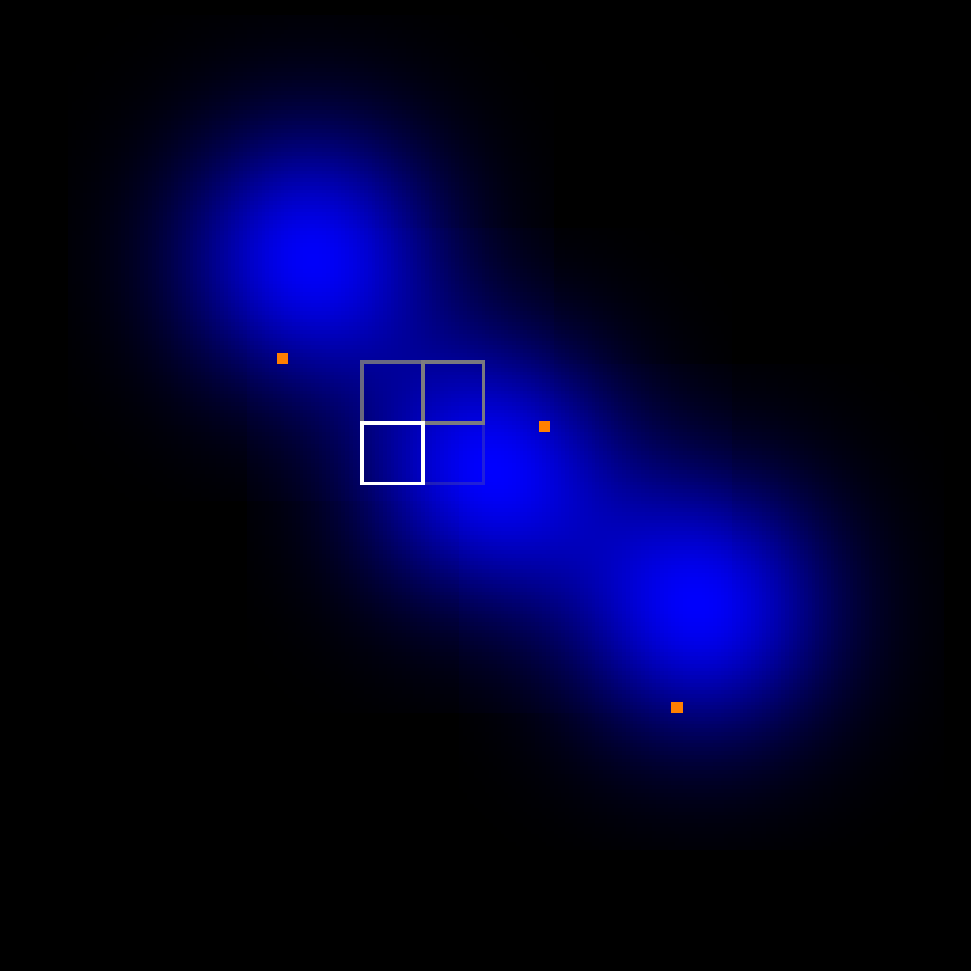
\includegraphics[interpolate=true,width=3.236667in,height=3.236667in]{gaussian-img0.png}}%
\end{pgfscope}%
\begin{pgfscope}%
\pgfpathrectangle{\pgfqpoint{0.705687in}{0.478947in}}{\pgfqpoint{3.233887in}{3.233887in}}%
\pgfusepath{clip}%
\pgfsetbuttcap%
\pgfsetmiterjoin%
\pgfsetlinewidth{0.752812pt}%
\definecolor{currentstroke}{rgb}{1.000000,0.000000,0.000000}%
\pgfsetstrokecolor{currentstroke}%
\pgfsetdash{{2.775000pt}{1.200000pt}}{0.000000pt}%
\pgfpathmoveto{\pgfqpoint{2.935301in}{1.543856in}}%
\pgfpathcurveto{\pgfqpoint{2.978183in}{1.543856in}}{\pgfqpoint{3.019314in}{1.526819in}}{\pgfqpoint{3.049636in}{1.496497in}}%
\pgfpathcurveto{\pgfqpoint{3.079958in}{1.466174in}}{\pgfqpoint{3.096995in}{1.425043in}}{\pgfqpoint{3.096995in}{1.382161in}}%
\pgfpathcurveto{\pgfqpoint{3.096995in}{1.339280in}}{\pgfqpoint{3.079958in}{1.298148in}}{\pgfqpoint{3.049636in}{1.267826in}}%
\pgfpathcurveto{\pgfqpoint{3.019314in}{1.237504in}}{\pgfqpoint{2.978183in}{1.220467in}}{\pgfqpoint{2.935301in}{1.220467in}}%
\pgfpathcurveto{\pgfqpoint{2.892419in}{1.220467in}}{\pgfqpoint{2.851288in}{1.237504in}}{\pgfqpoint{2.820966in}{1.267826in}}%
\pgfpathcurveto{\pgfqpoint{2.790644in}{1.298148in}}{\pgfqpoint{2.773606in}{1.339280in}}{\pgfqpoint{2.773606in}{1.382161in}}%
\pgfpathcurveto{\pgfqpoint{2.773606in}{1.425043in}}{\pgfqpoint{2.790644in}{1.466174in}}{\pgfqpoint{2.820966in}{1.496497in}}%
\pgfpathcurveto{\pgfqpoint{2.851288in}{1.526819in}}{\pgfqpoint{2.892419in}{1.543856in}}{\pgfqpoint{2.935301in}{1.543856in}}%
\pgfpathlineto{\pgfqpoint{2.935301in}{1.543856in}}%
\pgfpathclose%
\pgfusepath{stroke}%
\end{pgfscope}%
\begin{pgfscope}%
\pgfpathrectangle{\pgfqpoint{0.705687in}{0.478947in}}{\pgfqpoint{3.233887in}{3.233887in}}%
\pgfusepath{clip}%
\pgfsetbuttcap%
\pgfsetmiterjoin%
\pgfsetlinewidth{0.752812pt}%
\definecolor{currentstroke}{rgb}{1.000000,0.000000,0.000000}%
\pgfsetstrokecolor{currentstroke}%
\pgfsetdash{{2.775000pt}{1.200000pt}}{0.000000pt}%
\pgfpathmoveto{\pgfqpoint{1.621534in}{2.706034in}}%
\pgfpathcurveto{\pgfqpoint{1.664416in}{2.706034in}}{\pgfqpoint{1.705547in}{2.688997in}}{\pgfqpoint{1.735869in}{2.658675in}}%
\pgfpathcurveto{\pgfqpoint{1.766191in}{2.628353in}}{\pgfqpoint{1.783228in}{2.587221in}}{\pgfqpoint{1.783228in}{2.544340in}}%
\pgfpathcurveto{\pgfqpoint{1.783228in}{2.501458in}}{\pgfqpoint{1.766191in}{2.460327in}}{\pgfqpoint{1.735869in}{2.430004in}}%
\pgfpathcurveto{\pgfqpoint{1.705547in}{2.399682in}}{\pgfqpoint{1.664416in}{2.382645in}}{\pgfqpoint{1.621534in}{2.382645in}}%
\pgfpathcurveto{\pgfqpoint{1.578652in}{2.382645in}}{\pgfqpoint{1.537521in}{2.399682in}}{\pgfqpoint{1.507199in}{2.430004in}}%
\pgfpathcurveto{\pgfqpoint{1.476877in}{2.460327in}}{\pgfqpoint{1.459840in}{2.501458in}}{\pgfqpoint{1.459840in}{2.544340in}}%
\pgfpathcurveto{\pgfqpoint{1.459840in}{2.587221in}}{\pgfqpoint{1.476877in}{2.628353in}}{\pgfqpoint{1.507199in}{2.658675in}}%
\pgfpathcurveto{\pgfqpoint{1.537521in}{2.688997in}}{\pgfqpoint{1.578652in}{2.706034in}}{\pgfqpoint{1.621534in}{2.706034in}}%
\pgfpathlineto{\pgfqpoint{1.621534in}{2.706034in}}%
\pgfpathclose%
\pgfusepath{stroke}%
\end{pgfscope}%
\begin{pgfscope}%
\pgfpathrectangle{\pgfqpoint{0.705687in}{0.478947in}}{\pgfqpoint{3.233887in}{3.233887in}}%
\pgfusepath{clip}%
\pgfsetbuttcap%
\pgfsetmiterjoin%
\pgfsetlinewidth{0.752812pt}%
\definecolor{currentstroke}{rgb}{1.000000,0.000000,0.000000}%
\pgfsetstrokecolor{currentstroke}%
\pgfsetdash{{2.775000pt}{1.200000pt}}{0.000000pt}%
\pgfpathmoveto{\pgfqpoint{2.493168in}{2.478651in}}%
\pgfpathcurveto{\pgfqpoint{2.536050in}{2.478651in}}{\pgfqpoint{2.577181in}{2.461614in}}{\pgfqpoint{2.607503in}{2.431292in}}%
\pgfpathcurveto{\pgfqpoint{2.637825in}{2.400970in}}{\pgfqpoint{2.654862in}{2.359839in}}{\pgfqpoint{2.654862in}{2.316957in}}%
\pgfpathcurveto{\pgfqpoint{2.654862in}{2.274075in}}{\pgfqpoint{2.637825in}{2.232944in}}{\pgfqpoint{2.607503in}{2.202622in}}%
\pgfpathcurveto{\pgfqpoint{2.577181in}{2.172300in}}{\pgfqpoint{2.536050in}{2.155263in}}{\pgfqpoint{2.493168in}{2.155263in}}%
\pgfpathcurveto{\pgfqpoint{2.450286in}{2.155263in}}{\pgfqpoint{2.409155in}{2.172300in}}{\pgfqpoint{2.378833in}{2.202622in}}%
\pgfpathcurveto{\pgfqpoint{2.348511in}{2.232944in}}{\pgfqpoint{2.331473in}{2.274075in}}{\pgfqpoint{2.331473in}{2.316957in}}%
\pgfpathcurveto{\pgfqpoint{2.331473in}{2.359839in}}{\pgfqpoint{2.348511in}{2.400970in}}{\pgfqpoint{2.378833in}{2.431292in}}%
\pgfpathcurveto{\pgfqpoint{2.409155in}{2.461614in}}{\pgfqpoint{2.450286in}{2.478651in}}{\pgfqpoint{2.493168in}{2.478651in}}%
\pgfpathlineto{\pgfqpoint{2.493168in}{2.478651in}}%
\pgfpathclose%
\pgfusepath{stroke}%
\end{pgfscope}%
\begin{pgfscope}%
\pgfsetbuttcap%
\pgfsetroundjoin%
\definecolor{currentfill}{rgb}{0.000000,0.000000,0.000000}%
\pgfsetfillcolor{currentfill}%
\pgfsetlinewidth{0.803000pt}%
\definecolor{currentstroke}{rgb}{0.000000,0.000000,0.000000}%
\pgfsetstrokecolor{currentstroke}%
\pgfsetdash{}{0pt}%
\pgfsys@defobject{currentmarker}{\pgfqpoint{0.000000in}{-0.048611in}}{\pgfqpoint{0.000000in}{0.000000in}}{%
\pgfpathmoveto{\pgfqpoint{0.000000in}{0.000000in}}%
\pgfpathlineto{\pgfqpoint{0.000000in}{-0.048611in}}%
\pgfusepath{stroke,fill}%
}%
\begin{pgfscope}%
\pgfsys@transformshift{0.712003in}{0.478947in}%
\pgfsys@useobject{currentmarker}{}%
\end{pgfscope}%
\end{pgfscope}%
\begin{pgfscope}%
\definecolor{textcolor}{rgb}{0.000000,0.000000,0.000000}%
\pgfsetstrokecolor{textcolor}%
\pgfsetfillcolor{textcolor}%
\pgftext[x=0.712003in,y=0.381724in,,top]{\color{textcolor}\rmfamily\fontsize{8.000000}{9.600000}\selectfont \(\displaystyle {0}\)}%
\end{pgfscope}%
\begin{pgfscope}%
\pgfsetbuttcap%
\pgfsetroundjoin%
\definecolor{currentfill}{rgb}{0.000000,0.000000,0.000000}%
\pgfsetfillcolor{currentfill}%
\pgfsetlinewidth{0.803000pt}%
\definecolor{currentstroke}{rgb}{0.000000,0.000000,0.000000}%
\pgfsetstrokecolor{currentstroke}%
\pgfsetdash{}{0pt}%
\pgfsys@defobject{currentmarker}{\pgfqpoint{0.000000in}{-0.048611in}}{\pgfqpoint{0.000000in}{0.000000in}}{%
\pgfpathmoveto{\pgfqpoint{0.000000in}{0.000000in}}%
\pgfpathlineto{\pgfqpoint{0.000000in}{-0.048611in}}%
\pgfusepath{stroke,fill}%
}%
\begin{pgfscope}%
\pgfsys@transformshift{1.343622in}{0.478947in}%
\pgfsys@useobject{currentmarker}{}%
\end{pgfscope}%
\end{pgfscope}%
\begin{pgfscope}%
\definecolor{textcolor}{rgb}{0.000000,0.000000,0.000000}%
\pgfsetstrokecolor{textcolor}%
\pgfsetfillcolor{textcolor}%
\pgftext[x=1.343622in,y=0.381724in,,top]{\color{textcolor}\rmfamily\fontsize{8.000000}{9.600000}\selectfont \(\displaystyle {50}\)}%
\end{pgfscope}%
\begin{pgfscope}%
\pgfsetbuttcap%
\pgfsetroundjoin%
\definecolor{currentfill}{rgb}{0.000000,0.000000,0.000000}%
\pgfsetfillcolor{currentfill}%
\pgfsetlinewidth{0.803000pt}%
\definecolor{currentstroke}{rgb}{0.000000,0.000000,0.000000}%
\pgfsetstrokecolor{currentstroke}%
\pgfsetdash{}{0pt}%
\pgfsys@defobject{currentmarker}{\pgfqpoint{0.000000in}{-0.048611in}}{\pgfqpoint{0.000000in}{0.000000in}}{%
\pgfpathmoveto{\pgfqpoint{0.000000in}{0.000000in}}%
\pgfpathlineto{\pgfqpoint{0.000000in}{-0.048611in}}%
\pgfusepath{stroke,fill}%
}%
\begin{pgfscope}%
\pgfsys@transformshift{1.975240in}{0.478947in}%
\pgfsys@useobject{currentmarker}{}%
\end{pgfscope}%
\end{pgfscope}%
\begin{pgfscope}%
\definecolor{textcolor}{rgb}{0.000000,0.000000,0.000000}%
\pgfsetstrokecolor{textcolor}%
\pgfsetfillcolor{textcolor}%
\pgftext[x=1.975240in,y=0.381724in,,top]{\color{textcolor}\rmfamily\fontsize{8.000000}{9.600000}\selectfont \(\displaystyle {100}\)}%
\end{pgfscope}%
\begin{pgfscope}%
\pgfsetbuttcap%
\pgfsetroundjoin%
\definecolor{currentfill}{rgb}{0.000000,0.000000,0.000000}%
\pgfsetfillcolor{currentfill}%
\pgfsetlinewidth{0.803000pt}%
\definecolor{currentstroke}{rgb}{0.000000,0.000000,0.000000}%
\pgfsetstrokecolor{currentstroke}%
\pgfsetdash{}{0pt}%
\pgfsys@defobject{currentmarker}{\pgfqpoint{0.000000in}{-0.048611in}}{\pgfqpoint{0.000000in}{0.000000in}}{%
\pgfpathmoveto{\pgfqpoint{0.000000in}{0.000000in}}%
\pgfpathlineto{\pgfqpoint{0.000000in}{-0.048611in}}%
\pgfusepath{stroke,fill}%
}%
\begin{pgfscope}%
\pgfsys@transformshift{2.606859in}{0.478947in}%
\pgfsys@useobject{currentmarker}{}%
\end{pgfscope}%
\end{pgfscope}%
\begin{pgfscope}%
\definecolor{textcolor}{rgb}{0.000000,0.000000,0.000000}%
\pgfsetstrokecolor{textcolor}%
\pgfsetfillcolor{textcolor}%
\pgftext[x=2.606859in,y=0.381724in,,top]{\color{textcolor}\rmfamily\fontsize{8.000000}{9.600000}\selectfont \(\displaystyle {150}\)}%
\end{pgfscope}%
\begin{pgfscope}%
\pgfsetbuttcap%
\pgfsetroundjoin%
\definecolor{currentfill}{rgb}{0.000000,0.000000,0.000000}%
\pgfsetfillcolor{currentfill}%
\pgfsetlinewidth{0.803000pt}%
\definecolor{currentstroke}{rgb}{0.000000,0.000000,0.000000}%
\pgfsetstrokecolor{currentstroke}%
\pgfsetdash{}{0pt}%
\pgfsys@defobject{currentmarker}{\pgfqpoint{0.000000in}{-0.048611in}}{\pgfqpoint{0.000000in}{0.000000in}}{%
\pgfpathmoveto{\pgfqpoint{0.000000in}{0.000000in}}%
\pgfpathlineto{\pgfqpoint{0.000000in}{-0.048611in}}%
\pgfusepath{stroke,fill}%
}%
\begin{pgfscope}%
\pgfsys@transformshift{3.238478in}{0.478947in}%
\pgfsys@useobject{currentmarker}{}%
\end{pgfscope}%
\end{pgfscope}%
\begin{pgfscope}%
\definecolor{textcolor}{rgb}{0.000000,0.000000,0.000000}%
\pgfsetstrokecolor{textcolor}%
\pgfsetfillcolor{textcolor}%
\pgftext[x=3.238478in,y=0.381724in,,top]{\color{textcolor}\rmfamily\fontsize{8.000000}{9.600000}\selectfont \(\displaystyle {200}\)}%
\end{pgfscope}%
\begin{pgfscope}%
\pgfsetbuttcap%
\pgfsetroundjoin%
\definecolor{currentfill}{rgb}{0.000000,0.000000,0.000000}%
\pgfsetfillcolor{currentfill}%
\pgfsetlinewidth{0.803000pt}%
\definecolor{currentstroke}{rgb}{0.000000,0.000000,0.000000}%
\pgfsetstrokecolor{currentstroke}%
\pgfsetdash{}{0pt}%
\pgfsys@defobject{currentmarker}{\pgfqpoint{0.000000in}{-0.048611in}}{\pgfqpoint{0.000000in}{0.000000in}}{%
\pgfpathmoveto{\pgfqpoint{0.000000in}{0.000000in}}%
\pgfpathlineto{\pgfqpoint{0.000000in}{-0.048611in}}%
\pgfusepath{stroke,fill}%
}%
\begin{pgfscope}%
\pgfsys@transformshift{3.870096in}{0.478947in}%
\pgfsys@useobject{currentmarker}{}%
\end{pgfscope}%
\end{pgfscope}%
\begin{pgfscope}%
\definecolor{textcolor}{rgb}{0.000000,0.000000,0.000000}%
\pgfsetstrokecolor{textcolor}%
\pgfsetfillcolor{textcolor}%
\pgftext[x=3.870096in,y=0.381724in,,top]{\color{textcolor}\rmfamily\fontsize{8.000000}{9.600000}\selectfont \(\displaystyle {250}\)}%
\end{pgfscope}%
\begin{pgfscope}%
\pgfsetbuttcap%
\pgfsetroundjoin%
\definecolor{currentfill}{rgb}{0.000000,0.000000,0.000000}%
\pgfsetfillcolor{currentfill}%
\pgfsetlinewidth{0.803000pt}%
\definecolor{currentstroke}{rgb}{0.000000,0.000000,0.000000}%
\pgfsetstrokecolor{currentstroke}%
\pgfsetdash{}{0pt}%
\pgfsys@defobject{currentmarker}{\pgfqpoint{-0.048611in}{0.000000in}}{\pgfqpoint{-0.000000in}{0.000000in}}{%
\pgfpathmoveto{\pgfqpoint{-0.000000in}{0.000000in}}%
\pgfpathlineto{\pgfqpoint{-0.048611in}{0.000000in}}%
\pgfusepath{stroke,fill}%
}%
\begin{pgfscope}%
\pgfsys@transformshift{0.705687in}{3.706518in}%
\pgfsys@useobject{currentmarker}{}%
\end{pgfscope}%
\end{pgfscope}%
\begin{pgfscope}%
\definecolor{textcolor}{rgb}{0.000000,0.000000,0.000000}%
\pgfsetstrokecolor{textcolor}%
\pgfsetfillcolor{textcolor}%
\pgftext[x=0.549436in, y=3.664309in, left, base]{\color{textcolor}\rmfamily\fontsize{8.000000}{9.600000}\selectfont \(\displaystyle {0}\)}%
\end{pgfscope}%
\begin{pgfscope}%
\pgfsetbuttcap%
\pgfsetroundjoin%
\definecolor{currentfill}{rgb}{0.000000,0.000000,0.000000}%
\pgfsetfillcolor{currentfill}%
\pgfsetlinewidth{0.803000pt}%
\definecolor{currentstroke}{rgb}{0.000000,0.000000,0.000000}%
\pgfsetstrokecolor{currentstroke}%
\pgfsetdash{}{0pt}%
\pgfsys@defobject{currentmarker}{\pgfqpoint{-0.048611in}{0.000000in}}{\pgfqpoint{-0.000000in}{0.000000in}}{%
\pgfpathmoveto{\pgfqpoint{-0.000000in}{0.000000in}}%
\pgfpathlineto{\pgfqpoint{-0.048611in}{0.000000in}}%
\pgfusepath{stroke,fill}%
}%
\begin{pgfscope}%
\pgfsys@transformshift{0.705687in}{3.074899in}%
\pgfsys@useobject{currentmarker}{}%
\end{pgfscope}%
\end{pgfscope}%
\begin{pgfscope}%
\definecolor{textcolor}{rgb}{0.000000,0.000000,0.000000}%
\pgfsetstrokecolor{textcolor}%
\pgfsetfillcolor{textcolor}%
\pgftext[x=0.490408in, y=3.032690in, left, base]{\color{textcolor}\rmfamily\fontsize{8.000000}{9.600000}\selectfont \(\displaystyle {50}\)}%
\end{pgfscope}%
\begin{pgfscope}%
\pgfsetbuttcap%
\pgfsetroundjoin%
\definecolor{currentfill}{rgb}{0.000000,0.000000,0.000000}%
\pgfsetfillcolor{currentfill}%
\pgfsetlinewidth{0.803000pt}%
\definecolor{currentstroke}{rgb}{0.000000,0.000000,0.000000}%
\pgfsetstrokecolor{currentstroke}%
\pgfsetdash{}{0pt}%
\pgfsys@defobject{currentmarker}{\pgfqpoint{-0.048611in}{0.000000in}}{\pgfqpoint{-0.000000in}{0.000000in}}{%
\pgfpathmoveto{\pgfqpoint{-0.000000in}{0.000000in}}%
\pgfpathlineto{\pgfqpoint{-0.048611in}{0.000000in}}%
\pgfusepath{stroke,fill}%
}%
\begin{pgfscope}%
\pgfsys@transformshift{0.705687in}{2.443281in}%
\pgfsys@useobject{currentmarker}{}%
\end{pgfscope}%
\end{pgfscope}%
\begin{pgfscope}%
\definecolor{textcolor}{rgb}{0.000000,0.000000,0.000000}%
\pgfsetstrokecolor{textcolor}%
\pgfsetfillcolor{textcolor}%
\pgftext[x=0.431379in, y=2.401071in, left, base]{\color{textcolor}\rmfamily\fontsize{8.000000}{9.600000}\selectfont \(\displaystyle {100}\)}%
\end{pgfscope}%
\begin{pgfscope}%
\pgfsetbuttcap%
\pgfsetroundjoin%
\definecolor{currentfill}{rgb}{0.000000,0.000000,0.000000}%
\pgfsetfillcolor{currentfill}%
\pgfsetlinewidth{0.803000pt}%
\definecolor{currentstroke}{rgb}{0.000000,0.000000,0.000000}%
\pgfsetstrokecolor{currentstroke}%
\pgfsetdash{}{0pt}%
\pgfsys@defobject{currentmarker}{\pgfqpoint{-0.048611in}{0.000000in}}{\pgfqpoint{-0.000000in}{0.000000in}}{%
\pgfpathmoveto{\pgfqpoint{-0.000000in}{0.000000in}}%
\pgfpathlineto{\pgfqpoint{-0.048611in}{0.000000in}}%
\pgfusepath{stroke,fill}%
}%
\begin{pgfscope}%
\pgfsys@transformshift{0.705687in}{1.811662in}%
\pgfsys@useobject{currentmarker}{}%
\end{pgfscope}%
\end{pgfscope}%
\begin{pgfscope}%
\definecolor{textcolor}{rgb}{0.000000,0.000000,0.000000}%
\pgfsetstrokecolor{textcolor}%
\pgfsetfillcolor{textcolor}%
\pgftext[x=0.431379in, y=1.769453in, left, base]{\color{textcolor}\rmfamily\fontsize{8.000000}{9.600000}\selectfont \(\displaystyle {150}\)}%
\end{pgfscope}%
\begin{pgfscope}%
\pgfsetbuttcap%
\pgfsetroundjoin%
\definecolor{currentfill}{rgb}{0.000000,0.000000,0.000000}%
\pgfsetfillcolor{currentfill}%
\pgfsetlinewidth{0.803000pt}%
\definecolor{currentstroke}{rgb}{0.000000,0.000000,0.000000}%
\pgfsetstrokecolor{currentstroke}%
\pgfsetdash{}{0pt}%
\pgfsys@defobject{currentmarker}{\pgfqpoint{-0.048611in}{0.000000in}}{\pgfqpoint{-0.000000in}{0.000000in}}{%
\pgfpathmoveto{\pgfqpoint{-0.000000in}{0.000000in}}%
\pgfpathlineto{\pgfqpoint{-0.048611in}{0.000000in}}%
\pgfusepath{stroke,fill}%
}%
\begin{pgfscope}%
\pgfsys@transformshift{0.705687in}{1.180043in}%
\pgfsys@useobject{currentmarker}{}%
\end{pgfscope}%
\end{pgfscope}%
\begin{pgfscope}%
\definecolor{textcolor}{rgb}{0.000000,0.000000,0.000000}%
\pgfsetstrokecolor{textcolor}%
\pgfsetfillcolor{textcolor}%
\pgftext[x=0.431379in, y=1.137834in, left, base]{\color{textcolor}\rmfamily\fontsize{8.000000}{9.600000}\selectfont \(\displaystyle {200}\)}%
\end{pgfscope}%
\begin{pgfscope}%
\pgfsetbuttcap%
\pgfsetroundjoin%
\definecolor{currentfill}{rgb}{0.000000,0.000000,0.000000}%
\pgfsetfillcolor{currentfill}%
\pgfsetlinewidth{0.803000pt}%
\definecolor{currentstroke}{rgb}{0.000000,0.000000,0.000000}%
\pgfsetstrokecolor{currentstroke}%
\pgfsetdash{}{0pt}%
\pgfsys@defobject{currentmarker}{\pgfqpoint{-0.048611in}{0.000000in}}{\pgfqpoint{-0.000000in}{0.000000in}}{%
\pgfpathmoveto{\pgfqpoint{-0.000000in}{0.000000in}}%
\pgfpathlineto{\pgfqpoint{-0.048611in}{0.000000in}}%
\pgfusepath{stroke,fill}%
}%
\begin{pgfscope}%
\pgfsys@transformshift{0.705687in}{0.548425in}%
\pgfsys@useobject{currentmarker}{}%
\end{pgfscope}%
\end{pgfscope}%
\begin{pgfscope}%
\definecolor{textcolor}{rgb}{0.000000,0.000000,0.000000}%
\pgfsetstrokecolor{textcolor}%
\pgfsetfillcolor{textcolor}%
\pgftext[x=0.431379in, y=0.506216in, left, base]{\color{textcolor}\rmfamily\fontsize{8.000000}{9.600000}\selectfont \(\displaystyle {250}\)}%
\end{pgfscope}%
\begin{pgfscope}%
\pgfsetrectcap%
\pgfsetmiterjoin%
\pgfsetlinewidth{0.803000pt}%
\definecolor{currentstroke}{rgb}{0.000000,0.000000,0.000000}%
\pgfsetstrokecolor{currentstroke}%
\pgfsetdash{}{0pt}%
\pgfpathmoveto{\pgfqpoint{0.705687in}{0.478947in}}%
\pgfpathlineto{\pgfqpoint{0.705687in}{3.712834in}}%
\pgfusepath{stroke}%
\end{pgfscope}%
\begin{pgfscope}%
\pgfsetrectcap%
\pgfsetmiterjoin%
\pgfsetlinewidth{0.803000pt}%
\definecolor{currentstroke}{rgb}{0.000000,0.000000,0.000000}%
\pgfsetstrokecolor{currentstroke}%
\pgfsetdash{}{0pt}%
\pgfpathmoveto{\pgfqpoint{3.939574in}{0.478947in}}%
\pgfpathlineto{\pgfqpoint{3.939574in}{3.712834in}}%
\pgfusepath{stroke}%
\end{pgfscope}%
\begin{pgfscope}%
\pgfsetrectcap%
\pgfsetmiterjoin%
\pgfsetlinewidth{0.803000pt}%
\definecolor{currentstroke}{rgb}{0.000000,0.000000,0.000000}%
\pgfsetstrokecolor{currentstroke}%
\pgfsetdash{}{0pt}%
\pgfpathmoveto{\pgfqpoint{0.705687in}{0.478947in}}%
\pgfpathlineto{\pgfqpoint{3.939574in}{0.478947in}}%
\pgfusepath{stroke}%
\end{pgfscope}%
\begin{pgfscope}%
\pgfsetrectcap%
\pgfsetmiterjoin%
\pgfsetlinewidth{0.803000pt}%
\definecolor{currentstroke}{rgb}{0.000000,0.000000,0.000000}%
\pgfsetstrokecolor{currentstroke}%
\pgfsetdash{}{0pt}%
\pgfpathmoveto{\pgfqpoint{0.705687in}{3.712834in}}%
\pgfpathlineto{\pgfqpoint{3.939574in}{3.712834in}}%
\pgfusepath{stroke}%
\end{pgfscope}%
\begin{pgfscope}%
\pgfpathrectangle{\pgfqpoint{4.129803in}{2.771004in}}{\pgfqpoint{0.951143in}{0.951143in}}%
\pgfusepath{clip}%
\pgfsys@transformshift{4.129803in}{2.771004in}%
\pgftext[left,bottom]{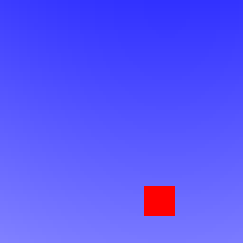
\includegraphics[interpolate=true,width=0.953333in,height=0.953333in]{gaussian-img1.png}}%
\end{pgfscope}%
\begin{pgfscope}%
\pgfpathrectangle{\pgfqpoint{4.129803in}{1.620319in}}{\pgfqpoint{0.951143in}{0.951143in}}%
\pgfusepath{clip}%
\pgfsys@transformshift{4.129803in}{1.620319in}%
\pgftext[left,bottom]{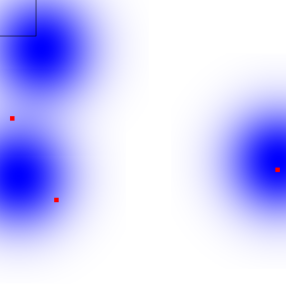
\includegraphics[interpolate=true,width=0.953333in,height=0.953333in]{gaussian-img2.png}}%
\end{pgfscope}%
\begin{pgfscope}%
\pgfpathrectangle{\pgfqpoint{4.129803in}{0.469634in}}{\pgfqpoint{0.951143in}{0.951143in}}%
\pgfusepath{clip}%
\pgfsys@transformshift{4.129803in}{0.469634in}%
\pgftext[left,bottom]{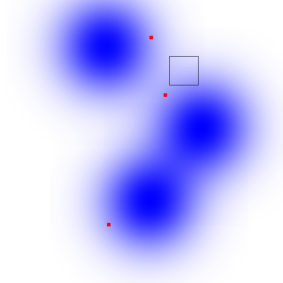
\includegraphics[interpolate=true,width=0.953333in,height=0.953333in]{gaussian-img3.png}}%
\end{pgfscope}%
\end{pgfpicture}%
\makeatother%
\endgroup%

    \label{fig:gaussian}
    %\vspace*{-1cm}
    \caption[Gaussian environment]{Four samples of the first environment. There are three gaussian kernels in the environment, whose height is visualized with the blue channel. There are three targets in the environment, whose location is sampled from the distribution defined by the sum of the three gaussian kernels.}
\end{figure}

\subsection{Terrain Environment}
% environment 2: medium, procedural and configurable

The second environment is intended to look like realistic terrain.
The scene's appearance is given by a \(512 \times 512\) RGB image.
The agent's view is a \(64 \times 64\) sub-image.
Gradient noise is generated and used as a height map.
The height map determines the color of the terrain.
The height also correlates to the probability of targets.
Specifically, targets are located between shores and mountain bases.
There are 10 targets in each scene.

The environment roughly corresponds to a UAV search-and-rescue scenario.
It is desirable that a searching agent should learn to not search oceans and lakes.
The agent should prioritize searching along the edges of land masses.
The appearance of the environment is highly configurable and has high variance.
We use this environment for evaluating the generalization capabilities of agents.

\begin{figure}
    \centering
    %% Creator: Matplotlib, PGF backend
%%
%% To include the figure in your LaTeX document, write
%%   \input{<filename>.pgf}
%%
%% Make sure the required packages are loaded in your preamble
%%   \usepackage{pgf}
%%
%% Also ensure that all the required font packages are loaded; for instance,
%% the lmodern package is sometimes necessary when using math font.
%%   \usepackage{lmodern}
%%
%% Figures using additional raster images can only be included by \input if
%% they are in the same directory as the main LaTeX file. For loading figures
%% from other directories you can use the `import` package
%%   \usepackage{import}
%%
%% and then include the figures with
%%   \import{<path to file>}{<filename>.pgf}
%%
%% Matplotlib used the following preamble
%%   \usepackage{fontspec}
%%   \setmainfont{DejaVuSerif.ttf}[Path=\detokenize{/usr/lib/python3.10/site-packages/matplotlib/mpl-data/fonts/ttf/}]
%%   \setsansfont{DejaVuSans.ttf}[Path=\detokenize{/usr/lib/python3.10/site-packages/matplotlib/mpl-data/fonts/ttf/}]
%%   \setmonofont{DejaVuSansMono.ttf}[Path=\detokenize{/usr/lib/python3.10/site-packages/matplotlib/mpl-data/fonts/ttf/}]
%%
\begingroup%
\makeatletter%
\begin{pgfpicture}%
\pgfpathrectangle{\pgfpointorigin}{\pgfqpoint{5.645496in}{4.234122in}}%
\pgfusepath{use as bounding box, clip}%
\begin{pgfscope}%
\pgfsetbuttcap%
\pgfsetmiterjoin%
\definecolor{currentfill}{rgb}{1.000000,1.000000,1.000000}%
\pgfsetfillcolor{currentfill}%
\pgfsetlinewidth{0.000000pt}%
\definecolor{currentstroke}{rgb}{1.000000,1.000000,1.000000}%
\pgfsetstrokecolor{currentstroke}%
\pgfsetdash{}{0pt}%
\pgfpathmoveto{\pgfqpoint{0.000000in}{0.000000in}}%
\pgfpathlineto{\pgfqpoint{5.645496in}{0.000000in}}%
\pgfpathlineto{\pgfqpoint{5.645496in}{4.234122in}}%
\pgfpathlineto{\pgfqpoint{0.000000in}{4.234122in}}%
\pgfpathlineto{\pgfqpoint{0.000000in}{0.000000in}}%
\pgfpathclose%
\pgfusepath{fill}%
\end{pgfscope}%
\begin{pgfscope}%
\pgfsetbuttcap%
\pgfsetmiterjoin%
\definecolor{currentfill}{rgb}{1.000000,1.000000,1.000000}%
\pgfsetfillcolor{currentfill}%
\pgfsetlinewidth{0.000000pt}%
\definecolor{currentstroke}{rgb}{0.000000,0.000000,0.000000}%
\pgfsetstrokecolor{currentstroke}%
\pgfsetstrokeopacity{0.000000}%
\pgfsetdash{}{0pt}%
\pgfpathmoveto{\pgfqpoint{0.705687in}{0.478947in}}%
\pgfpathlineto{\pgfqpoint{3.939574in}{0.478947in}}%
\pgfpathlineto{\pgfqpoint{3.939574in}{3.712834in}}%
\pgfpathlineto{\pgfqpoint{0.705687in}{3.712834in}}%
\pgfpathlineto{\pgfqpoint{0.705687in}{0.478947in}}%
\pgfpathclose%
\pgfusepath{fill}%
\end{pgfscope}%
\begin{pgfscope}%
\pgfpathrectangle{\pgfqpoint{0.705687in}{0.478947in}}{\pgfqpoint{3.233887in}{3.233887in}}%
\pgfusepath{clip}%
\pgfsys@transformshift{0.705687in}{0.478947in}%
\pgftext[left,bottom]{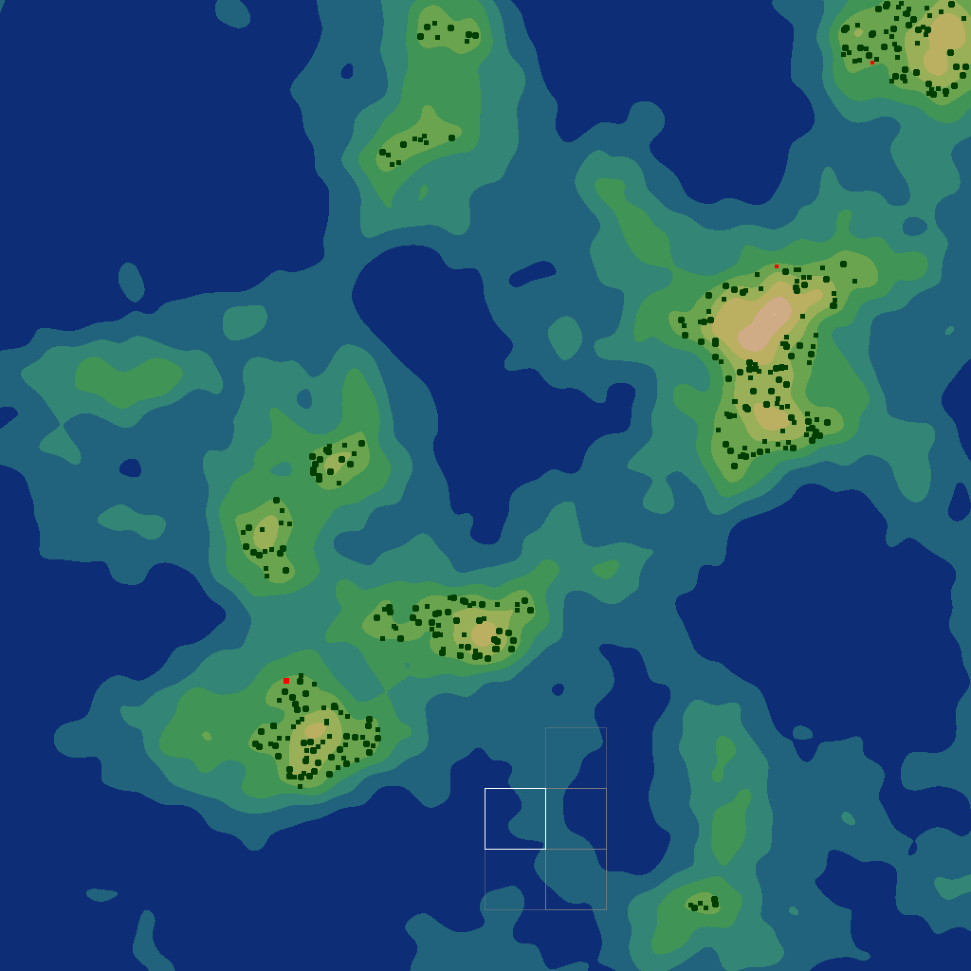
\includegraphics[interpolate=true,width=3.236667in,height=3.236667in]{terrain-img0.png}}%
\end{pgfscope}%
\begin{pgfscope}%
\pgfsetbuttcap%
\pgfsetroundjoin%
\definecolor{currentfill}{rgb}{0.000000,0.000000,0.000000}%
\pgfsetfillcolor{currentfill}%
\pgfsetlinewidth{0.803000pt}%
\definecolor{currentstroke}{rgb}{0.000000,0.000000,0.000000}%
\pgfsetstrokecolor{currentstroke}%
\pgfsetdash{}{0pt}%
\pgfsys@defobject{currentmarker}{\pgfqpoint{0.000000in}{-0.048611in}}{\pgfqpoint{0.000000in}{0.000000in}}{%
\pgfpathmoveto{\pgfqpoint{0.000000in}{0.000000in}}%
\pgfpathlineto{\pgfqpoint{0.000000in}{-0.048611in}}%
\pgfusepath{stroke,fill}%
}%
\begin{pgfscope}%
\pgfsys@transformshift{0.707266in}{0.478947in}%
\pgfsys@useobject{currentmarker}{}%
\end{pgfscope}%
\end{pgfscope}%
\begin{pgfscope}%
\definecolor{textcolor}{rgb}{0.000000,0.000000,0.000000}%
\pgfsetstrokecolor{textcolor}%
\pgfsetfillcolor{textcolor}%
\pgftext[x=0.707266in,y=0.381724in,,top]{\color{textcolor}\rmfamily\fontsize{8.000000}{9.600000}\selectfont \(\displaystyle {0}\)}%
\end{pgfscope}%
\begin{pgfscope}%
\pgfsetbuttcap%
\pgfsetroundjoin%
\definecolor{currentfill}{rgb}{0.000000,0.000000,0.000000}%
\pgfsetfillcolor{currentfill}%
\pgfsetlinewidth{0.803000pt}%
\definecolor{currentstroke}{rgb}{0.000000,0.000000,0.000000}%
\pgfsetstrokecolor{currentstroke}%
\pgfsetdash{}{0pt}%
\pgfsys@defobject{currentmarker}{\pgfqpoint{0.000000in}{-0.048611in}}{\pgfqpoint{0.000000in}{0.000000in}}{%
\pgfpathmoveto{\pgfqpoint{0.000000in}{0.000000in}}%
\pgfpathlineto{\pgfqpoint{0.000000in}{-0.048611in}}%
\pgfusepath{stroke,fill}%
}%
\begin{pgfscope}%
\pgfsys@transformshift{3.937995in}{0.478947in}%
\pgfsys@useobject{currentmarker}{}%
\end{pgfscope}%
\end{pgfscope}%
\begin{pgfscope}%
\definecolor{textcolor}{rgb}{0.000000,0.000000,0.000000}%
\pgfsetstrokecolor{textcolor}%
\pgfsetfillcolor{textcolor}%
\pgftext[x=3.937995in,y=0.381724in,,top]{\color{textcolor}\rmfamily\fontsize{8.000000}{9.600000}\selectfont \(\displaystyle {1023}\)}%
\end{pgfscope}%
\begin{pgfscope}%
\pgfsetbuttcap%
\pgfsetroundjoin%
\definecolor{currentfill}{rgb}{0.000000,0.000000,0.000000}%
\pgfsetfillcolor{currentfill}%
\pgfsetlinewidth{0.803000pt}%
\definecolor{currentstroke}{rgb}{0.000000,0.000000,0.000000}%
\pgfsetstrokecolor{currentstroke}%
\pgfsetdash{}{0pt}%
\pgfsys@defobject{currentmarker}{\pgfqpoint{-0.048611in}{0.000000in}}{\pgfqpoint{-0.000000in}{0.000000in}}{%
\pgfpathmoveto{\pgfqpoint{-0.000000in}{0.000000in}}%
\pgfpathlineto{\pgfqpoint{-0.048611in}{0.000000in}}%
\pgfusepath{stroke,fill}%
}%
\begin{pgfscope}%
\pgfsys@transformshift{0.705687in}{3.711255in}%
\pgfsys@useobject{currentmarker}{}%
\end{pgfscope}%
\end{pgfscope}%
\begin{pgfscope}%
\definecolor{textcolor}{rgb}{0.000000,0.000000,0.000000}%
\pgfsetstrokecolor{textcolor}%
\pgfsetfillcolor{textcolor}%
\pgftext[x=0.549436in, y=3.669046in, left, base]{\color{textcolor}\rmfamily\fontsize{8.000000}{9.600000}\selectfont \(\displaystyle {0}\)}%
\end{pgfscope}%
\begin{pgfscope}%
\pgfsetbuttcap%
\pgfsetroundjoin%
\definecolor{currentfill}{rgb}{0.000000,0.000000,0.000000}%
\pgfsetfillcolor{currentfill}%
\pgfsetlinewidth{0.803000pt}%
\definecolor{currentstroke}{rgb}{0.000000,0.000000,0.000000}%
\pgfsetstrokecolor{currentstroke}%
\pgfsetdash{}{0pt}%
\pgfsys@defobject{currentmarker}{\pgfqpoint{-0.048611in}{0.000000in}}{\pgfqpoint{-0.000000in}{0.000000in}}{%
\pgfpathmoveto{\pgfqpoint{-0.000000in}{0.000000in}}%
\pgfpathlineto{\pgfqpoint{-0.048611in}{0.000000in}}%
\pgfusepath{stroke,fill}%
}%
\begin{pgfscope}%
\pgfsys@transformshift{0.705687in}{0.480526in}%
\pgfsys@useobject{currentmarker}{}%
\end{pgfscope}%
\end{pgfscope}%
\begin{pgfscope}%
\definecolor{textcolor}{rgb}{0.000000,0.000000,0.000000}%
\pgfsetstrokecolor{textcolor}%
\pgfsetfillcolor{textcolor}%
\pgftext[x=0.372350in, y=0.438317in, left, base]{\color{textcolor}\rmfamily\fontsize{8.000000}{9.600000}\selectfont \(\displaystyle {1023}\)}%
\end{pgfscope}%
\begin{pgfscope}%
\pgfsetrectcap%
\pgfsetmiterjoin%
\pgfsetlinewidth{0.803000pt}%
\definecolor{currentstroke}{rgb}{0.000000,0.000000,0.000000}%
\pgfsetstrokecolor{currentstroke}%
\pgfsetdash{}{0pt}%
\pgfpathmoveto{\pgfqpoint{0.705687in}{0.478947in}}%
\pgfpathlineto{\pgfqpoint{0.705687in}{3.712834in}}%
\pgfusepath{stroke}%
\end{pgfscope}%
\begin{pgfscope}%
\pgfsetrectcap%
\pgfsetmiterjoin%
\pgfsetlinewidth{0.803000pt}%
\definecolor{currentstroke}{rgb}{0.000000,0.000000,0.000000}%
\pgfsetstrokecolor{currentstroke}%
\pgfsetdash{}{0pt}%
\pgfpathmoveto{\pgfqpoint{3.939574in}{0.478947in}}%
\pgfpathlineto{\pgfqpoint{3.939574in}{3.712834in}}%
\pgfusepath{stroke}%
\end{pgfscope}%
\begin{pgfscope}%
\pgfsetrectcap%
\pgfsetmiterjoin%
\pgfsetlinewidth{0.803000pt}%
\definecolor{currentstroke}{rgb}{0.000000,0.000000,0.000000}%
\pgfsetstrokecolor{currentstroke}%
\pgfsetdash{}{0pt}%
\pgfpathmoveto{\pgfqpoint{0.705687in}{0.478947in}}%
\pgfpathlineto{\pgfqpoint{3.939574in}{0.478947in}}%
\pgfusepath{stroke}%
\end{pgfscope}%
\begin{pgfscope}%
\pgfsetrectcap%
\pgfsetmiterjoin%
\pgfsetlinewidth{0.803000pt}%
\definecolor{currentstroke}{rgb}{0.000000,0.000000,0.000000}%
\pgfsetstrokecolor{currentstroke}%
\pgfsetdash{}{0pt}%
\pgfpathmoveto{\pgfqpoint{0.705687in}{3.712834in}}%
\pgfpathlineto{\pgfqpoint{3.939574in}{3.712834in}}%
\pgfusepath{stroke}%
\end{pgfscope}%
\begin{pgfscope}%
\pgfpathrectangle{\pgfqpoint{0.705687in}{0.478947in}}{\pgfqpoint{3.233887in}{3.233887in}}%
\pgfusepath{clip}%
\pgfsetbuttcap%
\pgfsetmiterjoin%
\pgfsetlinewidth{1.003750pt}%
\definecolor{currentstroke}{rgb}{0.000000,0.000000,0.000000}%
\pgfsetstrokecolor{currentstroke}%
\pgfsetstrokeopacity{0.500000}%
\pgfsetdash{}{0pt}%
\pgfpathmoveto{\pgfqpoint{1.515738in}{2.094311in}}%
\pgfpathlineto{\pgfqpoint{1.717856in}{2.094311in}}%
\pgfpathlineto{\pgfqpoint{1.717856in}{1.892193in}}%
\pgfpathlineto{\pgfqpoint{1.515738in}{1.892193in}}%
\pgfpathlineto{\pgfqpoint{1.515738in}{2.094311in}}%
\pgfpathclose%
\pgfusepath{stroke}%
\end{pgfscope}%
\begin{pgfscope}%
\pgfsetroundcap%
\pgfsetroundjoin%
\pgfsetlinewidth{1.003750pt}%
\definecolor{currentstroke}{rgb}{0.000000,0.000000,0.000000}%
\pgfsetstrokecolor{currentstroke}%
\pgfsetstrokeopacity{0.500000}%
\pgfsetdash{}{0pt}%
\pgfpathmoveto{\pgfqpoint{1.029076in}{1.610807in}}%
\pgfpathquadraticcurveto{\pgfqpoint{1.272407in}{1.852559in}}{\pgfqpoint{1.515738in}{2.094311in}}%
\pgfusepath{stroke}%
\end{pgfscope}%
\begin{pgfscope}%
\pgfsetroundcap%
\pgfsetroundjoin%
\pgfsetlinewidth{1.003750pt}%
\definecolor{currentstroke}{rgb}{0.000000,0.000000,0.000000}%
\pgfsetstrokecolor{currentstroke}%
\pgfsetstrokeopacity{0.500000}%
\pgfsetdash{}{0pt}%
\pgfpathmoveto{\pgfqpoint{1.837548in}{1.610807in}}%
\pgfpathquadraticcurveto{\pgfqpoint{1.777702in}{1.852559in}}{\pgfqpoint{1.717856in}{2.094311in}}%
\pgfusepath{stroke}%
\end{pgfscope}%
\begin{pgfscope}%
\pgfsetbuttcap%
\pgfsetmiterjoin%
\definecolor{currentfill}{rgb}{1.000000,1.000000,1.000000}%
\pgfsetfillcolor{currentfill}%
\pgfsetlinewidth{0.000000pt}%
\definecolor{currentstroke}{rgb}{0.000000,0.000000,0.000000}%
\pgfsetstrokecolor{currentstroke}%
\pgfsetstrokeopacity{0.000000}%
\pgfsetdash{}{0pt}%
\pgfpathmoveto{\pgfqpoint{1.029076in}{0.802335in}}%
\pgfpathlineto{\pgfqpoint{1.837548in}{0.802335in}}%
\pgfpathlineto{\pgfqpoint{1.837548in}{1.610807in}}%
\pgfpathlineto{\pgfqpoint{1.029076in}{1.610807in}}%
\pgfpathlineto{\pgfqpoint{1.029076in}{0.802335in}}%
\pgfpathclose%
\pgfusepath{fill}%
\end{pgfscope}%
\begin{pgfscope}%
\pgfpathrectangle{\pgfqpoint{1.029076in}{0.802335in}}{\pgfqpoint{0.808472in}{0.808472in}}%
\pgfusepath{clip}%
\pgfsys@transformshift{1.029076in}{0.802335in}%
\pgftext[left,bottom]{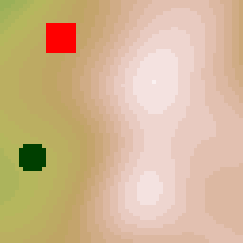
\includegraphics[interpolate=true,width=0.810000in,height=0.810000in]{terrain-img1.png}}%
\end{pgfscope}%
\begin{pgfscope}%
\pgfsetbuttcap%
\pgfsetroundjoin%
\definecolor{currentfill}{rgb}{0.000000,0.000000,0.000000}%
\pgfsetfillcolor{currentfill}%
\pgfsetlinewidth{0.803000pt}%
\definecolor{currentstroke}{rgb}{0.000000,0.000000,0.000000}%
\pgfsetstrokecolor{currentstroke}%
\pgfsetdash{}{0pt}%
\pgfsys@defobject{currentmarker}{\pgfqpoint{0.000000in}{-0.048611in}}{\pgfqpoint{0.000000in}{0.000000in}}{%
\pgfpathmoveto{\pgfqpoint{0.000000in}{0.000000in}}%
\pgfpathlineto{\pgfqpoint{0.000000in}{-0.048611in}}%
\pgfusepath{stroke,fill}%
}%
\begin{pgfscope}%
\pgfsys@transformshift{1.035392in}{0.802335in}%
\pgfsys@useobject{currentmarker}{}%
\end{pgfscope}%
\end{pgfscope}%
\begin{pgfscope}%
\definecolor{textcolor}{rgb}{0.000000,0.000000,0.000000}%
\pgfsetstrokecolor{textcolor}%
\pgfsetfillcolor{textcolor}%
\pgftext[x=1.035392in,y=0.705113in,,top]{\color{textcolor}\rmfamily\fontsize{8.000000}{9.600000}\selectfont \(\displaystyle {0}\)}%
\end{pgfscope}%
\begin{pgfscope}%
\pgfsetbuttcap%
\pgfsetroundjoin%
\definecolor{currentfill}{rgb}{0.000000,0.000000,0.000000}%
\pgfsetfillcolor{currentfill}%
\pgfsetlinewidth{0.803000pt}%
\definecolor{currentstroke}{rgb}{0.000000,0.000000,0.000000}%
\pgfsetstrokecolor{currentstroke}%
\pgfsetdash{}{0pt}%
\pgfsys@defobject{currentmarker}{\pgfqpoint{0.000000in}{-0.048611in}}{\pgfqpoint{0.000000in}{0.000000in}}{%
\pgfpathmoveto{\pgfqpoint{0.000000in}{0.000000in}}%
\pgfpathlineto{\pgfqpoint{0.000000in}{-0.048611in}}%
\pgfusepath{stroke,fill}%
}%
\begin{pgfscope}%
\pgfsys@transformshift{1.831231in}{0.802335in}%
\pgfsys@useobject{currentmarker}{}%
\end{pgfscope}%
\end{pgfscope}%
\begin{pgfscope}%
\definecolor{textcolor}{rgb}{0.000000,0.000000,0.000000}%
\pgfsetstrokecolor{textcolor}%
\pgfsetfillcolor{textcolor}%
\pgftext[x=1.831231in,y=0.705113in,,top]{\color{textcolor}\rmfamily\fontsize{8.000000}{9.600000}\selectfont \(\displaystyle {63}\)}%
\end{pgfscope}%
\begin{pgfscope}%
\pgfsetbuttcap%
\pgfsetroundjoin%
\definecolor{currentfill}{rgb}{0.000000,0.000000,0.000000}%
\pgfsetfillcolor{currentfill}%
\pgfsetlinewidth{0.803000pt}%
\definecolor{currentstroke}{rgb}{0.000000,0.000000,0.000000}%
\pgfsetstrokecolor{currentstroke}%
\pgfsetdash{}{0pt}%
\pgfsys@defobject{currentmarker}{\pgfqpoint{-0.048611in}{0.000000in}}{\pgfqpoint{-0.000000in}{0.000000in}}{%
\pgfpathmoveto{\pgfqpoint{-0.000000in}{0.000000in}}%
\pgfpathlineto{\pgfqpoint{-0.048611in}{0.000000in}}%
\pgfusepath{stroke,fill}%
}%
\begin{pgfscope}%
\pgfsys@transformshift{1.029076in}{1.604491in}%
\pgfsys@useobject{currentmarker}{}%
\end{pgfscope}%
\end{pgfscope}%
\begin{pgfscope}%
\definecolor{textcolor}{rgb}{0.000000,0.000000,0.000000}%
\pgfsetstrokecolor{textcolor}%
\pgfsetfillcolor{textcolor}%
\pgftext[x=0.872825in, y=1.562282in, left, base]{\color{textcolor}\rmfamily\fontsize{8.000000}{9.600000}\selectfont \(\displaystyle {0}\)}%
\end{pgfscope}%
\begin{pgfscope}%
\pgfsetbuttcap%
\pgfsetroundjoin%
\definecolor{currentfill}{rgb}{0.000000,0.000000,0.000000}%
\pgfsetfillcolor{currentfill}%
\pgfsetlinewidth{0.803000pt}%
\definecolor{currentstroke}{rgb}{0.000000,0.000000,0.000000}%
\pgfsetstrokecolor{currentstroke}%
\pgfsetdash{}{0pt}%
\pgfsys@defobject{currentmarker}{\pgfqpoint{-0.048611in}{0.000000in}}{\pgfqpoint{-0.000000in}{0.000000in}}{%
\pgfpathmoveto{\pgfqpoint{-0.000000in}{0.000000in}}%
\pgfpathlineto{\pgfqpoint{-0.048611in}{0.000000in}}%
\pgfusepath{stroke,fill}%
}%
\begin{pgfscope}%
\pgfsys@transformshift{1.029076in}{0.808652in}%
\pgfsys@useobject{currentmarker}{}%
\end{pgfscope}%
\end{pgfscope}%
\begin{pgfscope}%
\definecolor{textcolor}{rgb}{0.000000,0.000000,0.000000}%
\pgfsetstrokecolor{textcolor}%
\pgfsetfillcolor{textcolor}%
\pgftext[x=0.813796in, y=0.766442in, left, base]{\color{textcolor}\rmfamily\fontsize{8.000000}{9.600000}\selectfont \(\displaystyle {63}\)}%
\end{pgfscope}%
\begin{pgfscope}%
\pgfsetrectcap%
\pgfsetmiterjoin%
\pgfsetlinewidth{0.803000pt}%
\definecolor{currentstroke}{rgb}{0.000000,0.000000,0.000000}%
\pgfsetstrokecolor{currentstroke}%
\pgfsetdash{}{0pt}%
\pgfpathmoveto{\pgfqpoint{1.029076in}{0.802335in}}%
\pgfpathlineto{\pgfqpoint{1.029076in}{1.610807in}}%
\pgfusepath{stroke}%
\end{pgfscope}%
\begin{pgfscope}%
\pgfsetrectcap%
\pgfsetmiterjoin%
\pgfsetlinewidth{0.803000pt}%
\definecolor{currentstroke}{rgb}{0.000000,0.000000,0.000000}%
\pgfsetstrokecolor{currentstroke}%
\pgfsetdash{}{0pt}%
\pgfpathmoveto{\pgfqpoint{1.837548in}{0.802335in}}%
\pgfpathlineto{\pgfqpoint{1.837548in}{1.610807in}}%
\pgfusepath{stroke}%
\end{pgfscope}%
\begin{pgfscope}%
\pgfsetrectcap%
\pgfsetmiterjoin%
\pgfsetlinewidth{0.803000pt}%
\definecolor{currentstroke}{rgb}{0.000000,0.000000,0.000000}%
\pgfsetstrokecolor{currentstroke}%
\pgfsetdash{}{0pt}%
\pgfpathmoveto{\pgfqpoint{1.029076in}{0.802335in}}%
\pgfpathlineto{\pgfqpoint{1.837548in}{0.802335in}}%
\pgfusepath{stroke}%
\end{pgfscope}%
\begin{pgfscope}%
\pgfsetrectcap%
\pgfsetmiterjoin%
\pgfsetlinewidth{0.803000pt}%
\definecolor{currentstroke}{rgb}{0.000000,0.000000,0.000000}%
\pgfsetstrokecolor{currentstroke}%
\pgfsetdash{}{0pt}%
\pgfpathmoveto{\pgfqpoint{1.029076in}{1.610807in}}%
\pgfpathlineto{\pgfqpoint{1.837548in}{1.610807in}}%
\pgfusepath{stroke}%
\end{pgfscope}%
\begin{pgfscope}%
\pgfsetbuttcap%
\pgfsetmiterjoin%
\definecolor{currentfill}{rgb}{1.000000,1.000000,1.000000}%
\pgfsetfillcolor{currentfill}%
\pgfsetlinewidth{0.000000pt}%
\definecolor{currentstroke}{rgb}{0.000000,0.000000,0.000000}%
\pgfsetstrokecolor{currentstroke}%
\pgfsetstrokeopacity{0.000000}%
\pgfsetdash{}{0pt}%
\pgfpathmoveto{\pgfqpoint{4.129803in}{2.771004in}}%
\pgfpathlineto{\pgfqpoint{5.080946in}{2.771004in}}%
\pgfpathlineto{\pgfqpoint{5.080946in}{3.722147in}}%
\pgfpathlineto{\pgfqpoint{4.129803in}{3.722147in}}%
\pgfpathlineto{\pgfqpoint{4.129803in}{2.771004in}}%
\pgfpathclose%
\pgfusepath{fill}%
\end{pgfscope}%
\begin{pgfscope}%
\pgfpathrectangle{\pgfqpoint{4.129803in}{2.771004in}}{\pgfqpoint{0.951143in}{0.951143in}}%
\pgfusepath{clip}%
\pgfsys@transformshift{4.129803in}{2.771004in}%
\pgftext[left,bottom]{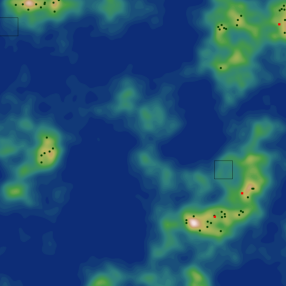
\includegraphics[interpolate=true,width=0.953333in,height=0.953333in]{terrain-img2.png}}%
\end{pgfscope}%
\begin{pgfscope}%
\pgfsetrectcap%
\pgfsetmiterjoin%
\pgfsetlinewidth{0.803000pt}%
\definecolor{currentstroke}{rgb}{0.000000,0.000000,0.000000}%
\pgfsetstrokecolor{currentstroke}%
\pgfsetdash{}{0pt}%
\pgfpathmoveto{\pgfqpoint{4.129803in}{2.771004in}}%
\pgfpathlineto{\pgfqpoint{4.129803in}{3.722147in}}%
\pgfusepath{stroke}%
\end{pgfscope}%
\begin{pgfscope}%
\pgfsetrectcap%
\pgfsetmiterjoin%
\pgfsetlinewidth{0.803000pt}%
\definecolor{currentstroke}{rgb}{0.000000,0.000000,0.000000}%
\pgfsetstrokecolor{currentstroke}%
\pgfsetdash{}{0pt}%
\pgfpathmoveto{\pgfqpoint{5.080946in}{2.771004in}}%
\pgfpathlineto{\pgfqpoint{5.080946in}{3.722147in}}%
\pgfusepath{stroke}%
\end{pgfscope}%
\begin{pgfscope}%
\pgfsetrectcap%
\pgfsetmiterjoin%
\pgfsetlinewidth{0.803000pt}%
\definecolor{currentstroke}{rgb}{0.000000,0.000000,0.000000}%
\pgfsetstrokecolor{currentstroke}%
\pgfsetdash{}{0pt}%
\pgfpathmoveto{\pgfqpoint{4.129803in}{2.771004in}}%
\pgfpathlineto{\pgfqpoint{5.080946in}{2.771004in}}%
\pgfusepath{stroke}%
\end{pgfscope}%
\begin{pgfscope}%
\pgfsetrectcap%
\pgfsetmiterjoin%
\pgfsetlinewidth{0.803000pt}%
\definecolor{currentstroke}{rgb}{0.000000,0.000000,0.000000}%
\pgfsetstrokecolor{currentstroke}%
\pgfsetdash{}{0pt}%
\pgfpathmoveto{\pgfqpoint{4.129803in}{3.722147in}}%
\pgfpathlineto{\pgfqpoint{5.080946in}{3.722147in}}%
\pgfusepath{stroke}%
\end{pgfscope}%
\begin{pgfscope}%
\pgfsetbuttcap%
\pgfsetmiterjoin%
\definecolor{currentfill}{rgb}{1.000000,1.000000,1.000000}%
\pgfsetfillcolor{currentfill}%
\pgfsetlinewidth{0.000000pt}%
\definecolor{currentstroke}{rgb}{0.000000,0.000000,0.000000}%
\pgfsetstrokecolor{currentstroke}%
\pgfsetstrokeopacity{0.000000}%
\pgfsetdash{}{0pt}%
\pgfpathmoveto{\pgfqpoint{4.129803in}{1.620319in}}%
\pgfpathlineto{\pgfqpoint{5.080946in}{1.620319in}}%
\pgfpathlineto{\pgfqpoint{5.080946in}{2.571462in}}%
\pgfpathlineto{\pgfqpoint{4.129803in}{2.571462in}}%
\pgfpathlineto{\pgfqpoint{4.129803in}{1.620319in}}%
\pgfpathclose%
\pgfusepath{fill}%
\end{pgfscope}%
\begin{pgfscope}%
\pgfpathrectangle{\pgfqpoint{4.129803in}{1.620319in}}{\pgfqpoint{0.951143in}{0.951143in}}%
\pgfusepath{clip}%
\pgfsys@transformshift{4.129803in}{1.620319in}%
\pgftext[left,bottom]{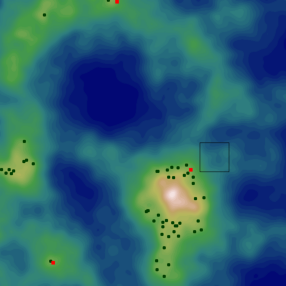
\includegraphics[interpolate=true,width=0.953333in,height=0.953333in]{terrain-img3.png}}%
\end{pgfscope}%
\begin{pgfscope}%
\pgfsetrectcap%
\pgfsetmiterjoin%
\pgfsetlinewidth{0.803000pt}%
\definecolor{currentstroke}{rgb}{0.000000,0.000000,0.000000}%
\pgfsetstrokecolor{currentstroke}%
\pgfsetdash{}{0pt}%
\pgfpathmoveto{\pgfqpoint{4.129803in}{1.620319in}}%
\pgfpathlineto{\pgfqpoint{4.129803in}{2.571462in}}%
\pgfusepath{stroke}%
\end{pgfscope}%
\begin{pgfscope}%
\pgfsetrectcap%
\pgfsetmiterjoin%
\pgfsetlinewidth{0.803000pt}%
\definecolor{currentstroke}{rgb}{0.000000,0.000000,0.000000}%
\pgfsetstrokecolor{currentstroke}%
\pgfsetdash{}{0pt}%
\pgfpathmoveto{\pgfqpoint{5.080946in}{1.620319in}}%
\pgfpathlineto{\pgfqpoint{5.080946in}{2.571462in}}%
\pgfusepath{stroke}%
\end{pgfscope}%
\begin{pgfscope}%
\pgfsetrectcap%
\pgfsetmiterjoin%
\pgfsetlinewidth{0.803000pt}%
\definecolor{currentstroke}{rgb}{0.000000,0.000000,0.000000}%
\pgfsetstrokecolor{currentstroke}%
\pgfsetdash{}{0pt}%
\pgfpathmoveto{\pgfqpoint{4.129803in}{1.620319in}}%
\pgfpathlineto{\pgfqpoint{5.080946in}{1.620319in}}%
\pgfusepath{stroke}%
\end{pgfscope}%
\begin{pgfscope}%
\pgfsetrectcap%
\pgfsetmiterjoin%
\pgfsetlinewidth{0.803000pt}%
\definecolor{currentstroke}{rgb}{0.000000,0.000000,0.000000}%
\pgfsetstrokecolor{currentstroke}%
\pgfsetdash{}{0pt}%
\pgfpathmoveto{\pgfqpoint{4.129803in}{2.571462in}}%
\pgfpathlineto{\pgfqpoint{5.080946in}{2.571462in}}%
\pgfusepath{stroke}%
\end{pgfscope}%
\begin{pgfscope}%
\pgfsetbuttcap%
\pgfsetmiterjoin%
\definecolor{currentfill}{rgb}{1.000000,1.000000,1.000000}%
\pgfsetfillcolor{currentfill}%
\pgfsetlinewidth{0.000000pt}%
\definecolor{currentstroke}{rgb}{0.000000,0.000000,0.000000}%
\pgfsetstrokecolor{currentstroke}%
\pgfsetstrokeopacity{0.000000}%
\pgfsetdash{}{0pt}%
\pgfpathmoveto{\pgfqpoint{4.129803in}{0.469634in}}%
\pgfpathlineto{\pgfqpoint{5.080946in}{0.469634in}}%
\pgfpathlineto{\pgfqpoint{5.080946in}{1.420777in}}%
\pgfpathlineto{\pgfqpoint{4.129803in}{1.420777in}}%
\pgfpathlineto{\pgfqpoint{4.129803in}{0.469634in}}%
\pgfpathclose%
\pgfusepath{fill}%
\end{pgfscope}%
\begin{pgfscope}%
\pgfpathrectangle{\pgfqpoint{4.129803in}{0.469634in}}{\pgfqpoint{0.951143in}{0.951143in}}%
\pgfusepath{clip}%
\pgfsys@transformshift{4.129803in}{0.469634in}%
\pgftext[left,bottom]{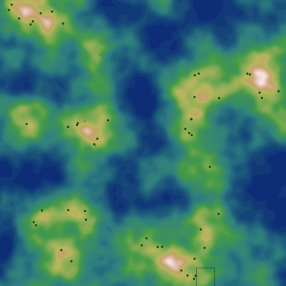
\includegraphics[interpolate=true,width=0.953333in,height=0.953333in]{terrain-img4.png}}%
\end{pgfscope}%
\begin{pgfscope}%
\pgfsetrectcap%
\pgfsetmiterjoin%
\pgfsetlinewidth{0.803000pt}%
\definecolor{currentstroke}{rgb}{0.000000,0.000000,0.000000}%
\pgfsetstrokecolor{currentstroke}%
\pgfsetdash{}{0pt}%
\pgfpathmoveto{\pgfqpoint{4.129803in}{0.469634in}}%
\pgfpathlineto{\pgfqpoint{4.129803in}{1.420777in}}%
\pgfusepath{stroke}%
\end{pgfscope}%
\begin{pgfscope}%
\pgfsetrectcap%
\pgfsetmiterjoin%
\pgfsetlinewidth{0.803000pt}%
\definecolor{currentstroke}{rgb}{0.000000,0.000000,0.000000}%
\pgfsetstrokecolor{currentstroke}%
\pgfsetdash{}{0pt}%
\pgfpathmoveto{\pgfqpoint{5.080946in}{0.469634in}}%
\pgfpathlineto{\pgfqpoint{5.080946in}{1.420777in}}%
\pgfusepath{stroke}%
\end{pgfscope}%
\begin{pgfscope}%
\pgfsetrectcap%
\pgfsetmiterjoin%
\pgfsetlinewidth{0.803000pt}%
\definecolor{currentstroke}{rgb}{0.000000,0.000000,0.000000}%
\pgfsetstrokecolor{currentstroke}%
\pgfsetdash{}{0pt}%
\pgfpathmoveto{\pgfqpoint{4.129803in}{0.469634in}}%
\pgfpathlineto{\pgfqpoint{5.080946in}{0.469634in}}%
\pgfusepath{stroke}%
\end{pgfscope}%
\begin{pgfscope}%
\pgfsetrectcap%
\pgfsetmiterjoin%
\pgfsetlinewidth{0.803000pt}%
\definecolor{currentstroke}{rgb}{0.000000,0.000000,0.000000}%
\pgfsetstrokecolor{currentstroke}%
\pgfsetdash{}{0pt}%
\pgfpathmoveto{\pgfqpoint{4.129803in}{1.420777in}}%
\pgfpathlineto{\pgfqpoint{5.080946in}{1.420777in}}%
\pgfusepath{stroke}%
\end{pgfscope}%
\end{pgfpicture}%
\makeatother%
\endgroup%

    \label{fig:terrain}
    %\vspace*{-1cm}
    \caption[Terrain environment]{Three samples of the terrain environment. Terrain seen from above with red targets scattered along island edges. The white border indicates the agent's current view.}
\end{figure}

\subsection{Camera Environment}
% environment 3: hard, realistic

The third environment is a three-dimensional version of the second one.
The heightmap is turned into a three-dimensional mesh, and the agent is placed at its center.
The agent observes the scene through a perspective projection pan-tilt camera.
Targets are, as before, placed along island edges.
The agent is therefore expected to avoid searching the skies and oceans.

This environment is intended to model more realistic scenarios where the image is more difficult to interpret.

\begin{figure}
    \centering
    %% Creator: Matplotlib, PGF backend
%%
%% To include the figure in your LaTeX document, write
%%   \input{<filename>.pgf}
%%
%% Make sure the required packages are loaded in your preamble
%%   \usepackage{pgf}
%%
%% Also ensure that all the required font packages are loaded; for instance,
%% the lmodern package is sometimes necessary when using math font.
%%   \usepackage{lmodern}
%%
%% Figures using additional raster images can only be included by \input if
%% they are in the same directory as the main LaTeX file. For loading figures
%% from other directories you can use the `import` package
%%   \usepackage{import}
%%
%% and then include the figures with
%%   \import{<path to file>}{<filename>.pgf}
%%
%% Matplotlib used the following preamble
%%   \usepackage{fontspec}
%%   \setmainfont{DejaVuSerif.ttf}[Path=\detokenize{/usr/lib/python3.10/site-packages/matplotlib/mpl-data/fonts/ttf/}]
%%   \setsansfont{DejaVuSans.ttf}[Path=\detokenize{/usr/lib/python3.10/site-packages/matplotlib/mpl-data/fonts/ttf/}]
%%   \setmonofont{DejaVuSansMono.ttf}[Path=\detokenize{/usr/lib/python3.10/site-packages/matplotlib/mpl-data/fonts/ttf/}]
%%
\begingroup%
\makeatletter%
\begin{pgfpicture}%
\pgfpathrectangle{\pgfpointorigin}{\pgfqpoint{5.645496in}{4.234122in}}%
\pgfusepath{use as bounding box, clip}%
\begin{pgfscope}%
\pgfsetbuttcap%
\pgfsetmiterjoin%
\definecolor{currentfill}{rgb}{1.000000,1.000000,1.000000}%
\pgfsetfillcolor{currentfill}%
\pgfsetlinewidth{0.000000pt}%
\definecolor{currentstroke}{rgb}{1.000000,1.000000,1.000000}%
\pgfsetstrokecolor{currentstroke}%
\pgfsetdash{}{0pt}%
\pgfpathmoveto{\pgfqpoint{0.000000in}{0.000000in}}%
\pgfpathlineto{\pgfqpoint{5.645496in}{0.000000in}}%
\pgfpathlineto{\pgfqpoint{5.645496in}{4.234122in}}%
\pgfpathlineto{\pgfqpoint{0.000000in}{4.234122in}}%
\pgfpathlineto{\pgfqpoint{0.000000in}{0.000000in}}%
\pgfpathclose%
\pgfusepath{fill}%
\end{pgfscope}%
\begin{pgfscope}%
\pgfsetbuttcap%
\pgfsetmiterjoin%
\definecolor{currentfill}{rgb}{1.000000,1.000000,1.000000}%
\pgfsetfillcolor{currentfill}%
\pgfsetlinewidth{0.000000pt}%
\definecolor{currentstroke}{rgb}{0.000000,0.000000,0.000000}%
\pgfsetstrokecolor{currentstroke}%
\pgfsetstrokeopacity{0.000000}%
\pgfsetdash{}{0pt}%
\pgfpathmoveto{\pgfqpoint{0.705687in}{0.478947in}}%
\pgfpathlineto{\pgfqpoint{3.939574in}{0.478947in}}%
\pgfpathlineto{\pgfqpoint{3.939574in}{3.712834in}}%
\pgfpathlineto{\pgfqpoint{0.705687in}{3.712834in}}%
\pgfpathlineto{\pgfqpoint{0.705687in}{0.478947in}}%
\pgfpathclose%
\pgfusepath{fill}%
\end{pgfscope}%
\begin{pgfscope}%
\pgfpathrectangle{\pgfqpoint{0.705687in}{0.478947in}}{\pgfqpoint{3.233887in}{3.233887in}}%
\pgfusepath{clip}%
\pgfsys@transformshift{0.705687in}{0.478947in}%
\pgftext[left,bottom]{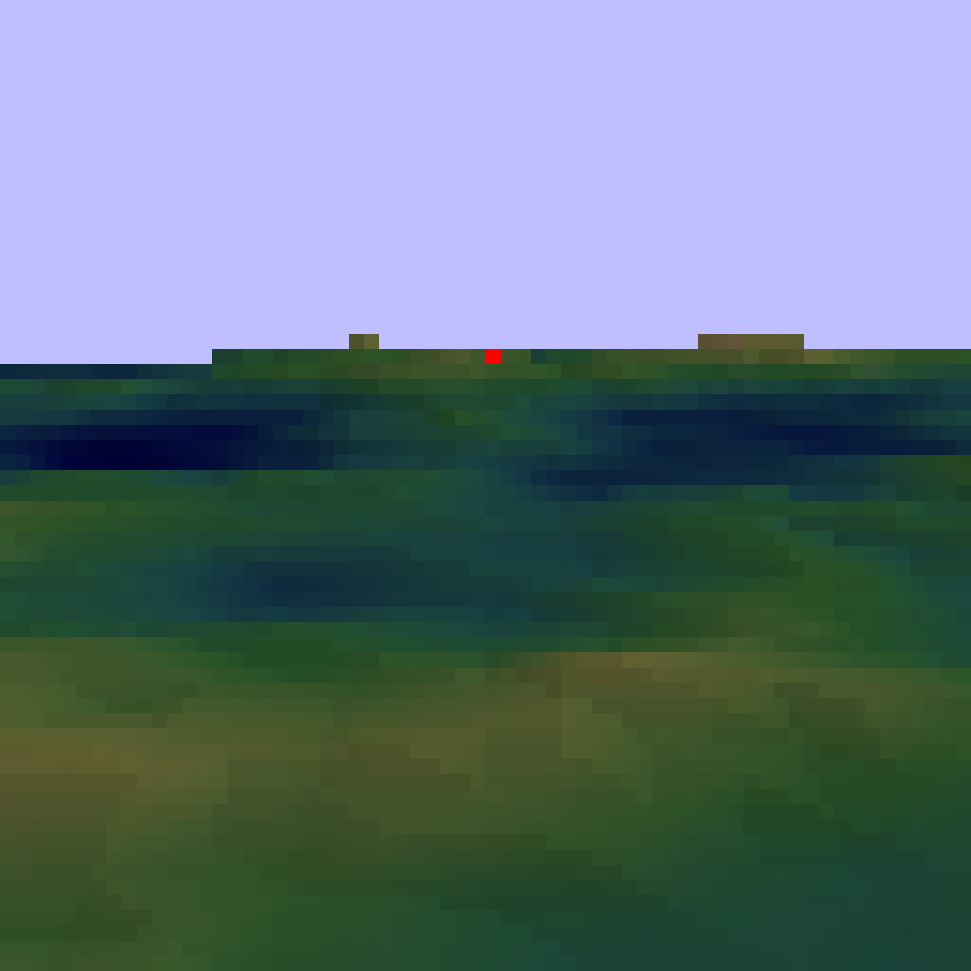
\includegraphics[interpolate=true,width=3.236667in,height=3.236667in]{camera-img0.png}}%
\end{pgfscope}%
\begin{pgfscope}%
\pgfsetbuttcap%
\pgfsetroundjoin%
\definecolor{currentfill}{rgb}{0.000000,0.000000,0.000000}%
\pgfsetfillcolor{currentfill}%
\pgfsetlinewidth{0.803000pt}%
\definecolor{currentstroke}{rgb}{0.000000,0.000000,0.000000}%
\pgfsetstrokecolor{currentstroke}%
\pgfsetdash{}{0pt}%
\pgfsys@defobject{currentmarker}{\pgfqpoint{0.000000in}{-0.048611in}}{\pgfqpoint{0.000000in}{0.000000in}}{%
\pgfpathmoveto{\pgfqpoint{0.000000in}{0.000000in}}%
\pgfpathlineto{\pgfqpoint{0.000000in}{-0.048611in}}%
\pgfusepath{stroke,fill}%
}%
\begin{pgfscope}%
\pgfsys@transformshift{0.730952in}{0.478947in}%
\pgfsys@useobject{currentmarker}{}%
\end{pgfscope}%
\end{pgfscope}%
\begin{pgfscope}%
\definecolor{textcolor}{rgb}{0.000000,0.000000,0.000000}%
\pgfsetstrokecolor{textcolor}%
\pgfsetfillcolor{textcolor}%
\pgftext[x=0.730952in,y=0.381724in,,top]{\color{textcolor}\rmfamily\fontsize{8.000000}{9.600000}\selectfont \(\displaystyle {0}\)}%
\end{pgfscope}%
\begin{pgfscope}%
\pgfsetbuttcap%
\pgfsetroundjoin%
\definecolor{currentfill}{rgb}{0.000000,0.000000,0.000000}%
\pgfsetfillcolor{currentfill}%
\pgfsetlinewidth{0.803000pt}%
\definecolor{currentstroke}{rgb}{0.000000,0.000000,0.000000}%
\pgfsetstrokecolor{currentstroke}%
\pgfsetdash{}{0pt}%
\pgfsys@defobject{currentmarker}{\pgfqpoint{0.000000in}{-0.048611in}}{\pgfqpoint{0.000000in}{0.000000in}}{%
\pgfpathmoveto{\pgfqpoint{0.000000in}{0.000000in}}%
\pgfpathlineto{\pgfqpoint{0.000000in}{-0.048611in}}%
\pgfusepath{stroke,fill}%
}%
\begin{pgfscope}%
\pgfsys@transformshift{3.914310in}{0.478947in}%
\pgfsys@useobject{currentmarker}{}%
\end{pgfscope}%
\end{pgfscope}%
\begin{pgfscope}%
\definecolor{textcolor}{rgb}{0.000000,0.000000,0.000000}%
\pgfsetstrokecolor{textcolor}%
\pgfsetfillcolor{textcolor}%
\pgftext[x=3.914310in,y=0.381724in,,top]{\color{textcolor}\rmfamily\fontsize{8.000000}{9.600000}\selectfont \(\displaystyle {63}\)}%
\end{pgfscope}%
\begin{pgfscope}%
\pgfsetbuttcap%
\pgfsetroundjoin%
\definecolor{currentfill}{rgb}{0.000000,0.000000,0.000000}%
\pgfsetfillcolor{currentfill}%
\pgfsetlinewidth{0.803000pt}%
\definecolor{currentstroke}{rgb}{0.000000,0.000000,0.000000}%
\pgfsetstrokecolor{currentstroke}%
\pgfsetdash{}{0pt}%
\pgfsys@defobject{currentmarker}{\pgfqpoint{-0.048611in}{0.000000in}}{\pgfqpoint{-0.000000in}{0.000000in}}{%
\pgfpathmoveto{\pgfqpoint{-0.000000in}{0.000000in}}%
\pgfpathlineto{\pgfqpoint{-0.048611in}{0.000000in}}%
\pgfusepath{stroke,fill}%
}%
\begin{pgfscope}%
\pgfsys@transformshift{0.705687in}{3.687569in}%
\pgfsys@useobject{currentmarker}{}%
\end{pgfscope}%
\end{pgfscope}%
\begin{pgfscope}%
\definecolor{textcolor}{rgb}{0.000000,0.000000,0.000000}%
\pgfsetstrokecolor{textcolor}%
\pgfsetfillcolor{textcolor}%
\pgftext[x=0.549436in, y=3.645360in, left, base]{\color{textcolor}\rmfamily\fontsize{8.000000}{9.600000}\selectfont \(\displaystyle {0}\)}%
\end{pgfscope}%
\begin{pgfscope}%
\pgfsetbuttcap%
\pgfsetroundjoin%
\definecolor{currentfill}{rgb}{0.000000,0.000000,0.000000}%
\pgfsetfillcolor{currentfill}%
\pgfsetlinewidth{0.803000pt}%
\definecolor{currentstroke}{rgb}{0.000000,0.000000,0.000000}%
\pgfsetstrokecolor{currentstroke}%
\pgfsetdash{}{0pt}%
\pgfsys@defobject{currentmarker}{\pgfqpoint{-0.048611in}{0.000000in}}{\pgfqpoint{-0.000000in}{0.000000in}}{%
\pgfpathmoveto{\pgfqpoint{-0.000000in}{0.000000in}}%
\pgfpathlineto{\pgfqpoint{-0.048611in}{0.000000in}}%
\pgfusepath{stroke,fill}%
}%
\begin{pgfscope}%
\pgfsys@transformshift{0.705687in}{0.504211in}%
\pgfsys@useobject{currentmarker}{}%
\end{pgfscope}%
\end{pgfscope}%
\begin{pgfscope}%
\definecolor{textcolor}{rgb}{0.000000,0.000000,0.000000}%
\pgfsetstrokecolor{textcolor}%
\pgfsetfillcolor{textcolor}%
\pgftext[x=0.490408in, y=0.462002in, left, base]{\color{textcolor}\rmfamily\fontsize{8.000000}{9.600000}\selectfont \(\displaystyle {63}\)}%
\end{pgfscope}%
\begin{pgfscope}%
\pgfsetrectcap%
\pgfsetmiterjoin%
\pgfsetlinewidth{0.803000pt}%
\definecolor{currentstroke}{rgb}{0.000000,0.000000,0.000000}%
\pgfsetstrokecolor{currentstroke}%
\pgfsetdash{}{0pt}%
\pgfpathmoveto{\pgfqpoint{0.705687in}{0.478947in}}%
\pgfpathlineto{\pgfqpoint{0.705687in}{3.712834in}}%
\pgfusepath{stroke}%
\end{pgfscope}%
\begin{pgfscope}%
\pgfsetrectcap%
\pgfsetmiterjoin%
\pgfsetlinewidth{0.803000pt}%
\definecolor{currentstroke}{rgb}{0.000000,0.000000,0.000000}%
\pgfsetstrokecolor{currentstroke}%
\pgfsetdash{}{0pt}%
\pgfpathmoveto{\pgfqpoint{3.939574in}{0.478947in}}%
\pgfpathlineto{\pgfqpoint{3.939574in}{3.712834in}}%
\pgfusepath{stroke}%
\end{pgfscope}%
\begin{pgfscope}%
\pgfsetrectcap%
\pgfsetmiterjoin%
\pgfsetlinewidth{0.803000pt}%
\definecolor{currentstroke}{rgb}{0.000000,0.000000,0.000000}%
\pgfsetstrokecolor{currentstroke}%
\pgfsetdash{}{0pt}%
\pgfpathmoveto{\pgfqpoint{0.705687in}{0.478947in}}%
\pgfpathlineto{\pgfqpoint{3.939574in}{0.478947in}}%
\pgfusepath{stroke}%
\end{pgfscope}%
\begin{pgfscope}%
\pgfsetrectcap%
\pgfsetmiterjoin%
\pgfsetlinewidth{0.803000pt}%
\definecolor{currentstroke}{rgb}{0.000000,0.000000,0.000000}%
\pgfsetstrokecolor{currentstroke}%
\pgfsetdash{}{0pt}%
\pgfpathmoveto{\pgfqpoint{0.705687in}{3.712834in}}%
\pgfpathlineto{\pgfqpoint{3.939574in}{3.712834in}}%
\pgfusepath{stroke}%
\end{pgfscope}%
\begin{pgfscope}%
\pgfsetbuttcap%
\pgfsetmiterjoin%
\definecolor{currentfill}{rgb}{1.000000,1.000000,1.000000}%
\pgfsetfillcolor{currentfill}%
\pgfsetlinewidth{0.000000pt}%
\definecolor{currentstroke}{rgb}{0.000000,0.000000,0.000000}%
\pgfsetstrokecolor{currentstroke}%
\pgfsetstrokeopacity{0.000000}%
\pgfsetdash{}{0pt}%
\pgfpathmoveto{\pgfqpoint{4.129803in}{2.767123in}}%
\pgfpathlineto{\pgfqpoint{5.080946in}{2.767123in}}%
\pgfpathlineto{\pgfqpoint{5.080946in}{3.726027in}}%
\pgfpathlineto{\pgfqpoint{4.129803in}{3.726027in}}%
\pgfpathlineto{\pgfqpoint{4.129803in}{2.767123in}}%
\pgfpathclose%
\pgfusepath{fill}%
\end{pgfscope}%
\begin{pgfscope}%
\pgfsetbuttcap%
\pgfsetroundjoin%
\definecolor{currentfill}{rgb}{0.000000,0.000000,0.000000}%
\pgfsetfillcolor{currentfill}%
\pgfsetlinewidth{0.803000pt}%
\definecolor{currentstroke}{rgb}{0.000000,0.000000,0.000000}%
\pgfsetstrokecolor{currentstroke}%
\pgfsetdash{}{0pt}%
\pgfsys@defobject{currentmarker}{\pgfqpoint{0.000000in}{-0.048611in}}{\pgfqpoint{0.000000in}{0.000000in}}{%
\pgfpathmoveto{\pgfqpoint{0.000000in}{0.000000in}}%
\pgfpathlineto{\pgfqpoint{0.000000in}{-0.048611in}}%
\pgfusepath{stroke,fill}%
}%
\begin{pgfscope}%
\pgfsys@transformshift{4.129803in}{2.767123in}%
\pgfsys@useobject{currentmarker}{}%
\end{pgfscope}%
\end{pgfscope}%
\begin{pgfscope}%
\definecolor{textcolor}{rgb}{0.000000,0.000000,0.000000}%
\pgfsetstrokecolor{textcolor}%
\pgfsetfillcolor{textcolor}%
\pgftext[x=4.129803in,y=2.669901in,,top]{\color{textcolor}\rmfamily\fontsize{8.000000}{9.600000}\selectfont \(\displaystyle {0.0}\)}%
\end{pgfscope}%
\begin{pgfscope}%
\pgfsetbuttcap%
\pgfsetroundjoin%
\definecolor{currentfill}{rgb}{0.000000,0.000000,0.000000}%
\pgfsetfillcolor{currentfill}%
\pgfsetlinewidth{0.803000pt}%
\definecolor{currentstroke}{rgb}{0.000000,0.000000,0.000000}%
\pgfsetstrokecolor{currentstroke}%
\pgfsetdash{}{0pt}%
\pgfsys@defobject{currentmarker}{\pgfqpoint{0.000000in}{-0.048611in}}{\pgfqpoint{0.000000in}{0.000000in}}{%
\pgfpathmoveto{\pgfqpoint{0.000000in}{0.000000in}}%
\pgfpathlineto{\pgfqpoint{0.000000in}{-0.048611in}}%
\pgfusepath{stroke,fill}%
}%
\begin{pgfscope}%
\pgfsys@transformshift{4.605375in}{2.767123in}%
\pgfsys@useobject{currentmarker}{}%
\end{pgfscope}%
\end{pgfscope}%
\begin{pgfscope}%
\definecolor{textcolor}{rgb}{0.000000,0.000000,0.000000}%
\pgfsetstrokecolor{textcolor}%
\pgfsetfillcolor{textcolor}%
\pgftext[x=4.605375in,y=2.669901in,,top]{\color{textcolor}\rmfamily\fontsize{8.000000}{9.600000}\selectfont \(\displaystyle {0.5}\)}%
\end{pgfscope}%
\begin{pgfscope}%
\pgfsetbuttcap%
\pgfsetroundjoin%
\definecolor{currentfill}{rgb}{0.000000,0.000000,0.000000}%
\pgfsetfillcolor{currentfill}%
\pgfsetlinewidth{0.803000pt}%
\definecolor{currentstroke}{rgb}{0.000000,0.000000,0.000000}%
\pgfsetstrokecolor{currentstroke}%
\pgfsetdash{}{0pt}%
\pgfsys@defobject{currentmarker}{\pgfqpoint{0.000000in}{-0.048611in}}{\pgfqpoint{0.000000in}{0.000000in}}{%
\pgfpathmoveto{\pgfqpoint{0.000000in}{0.000000in}}%
\pgfpathlineto{\pgfqpoint{0.000000in}{-0.048611in}}%
\pgfusepath{stroke,fill}%
}%
\begin{pgfscope}%
\pgfsys@transformshift{5.080946in}{2.767123in}%
\pgfsys@useobject{currentmarker}{}%
\end{pgfscope}%
\end{pgfscope}%
\begin{pgfscope}%
\definecolor{textcolor}{rgb}{0.000000,0.000000,0.000000}%
\pgfsetstrokecolor{textcolor}%
\pgfsetfillcolor{textcolor}%
\pgftext[x=5.080946in,y=2.669901in,,top]{\color{textcolor}\rmfamily\fontsize{8.000000}{9.600000}\selectfont \(\displaystyle {1.0}\)}%
\end{pgfscope}%
\begin{pgfscope}%
\pgfsetbuttcap%
\pgfsetroundjoin%
\definecolor{currentfill}{rgb}{0.000000,0.000000,0.000000}%
\pgfsetfillcolor{currentfill}%
\pgfsetlinewidth{0.803000pt}%
\definecolor{currentstroke}{rgb}{0.000000,0.000000,0.000000}%
\pgfsetstrokecolor{currentstroke}%
\pgfsetdash{}{0pt}%
\pgfsys@defobject{currentmarker}{\pgfqpoint{-0.048611in}{0.000000in}}{\pgfqpoint{-0.000000in}{0.000000in}}{%
\pgfpathmoveto{\pgfqpoint{-0.000000in}{0.000000in}}%
\pgfpathlineto{\pgfqpoint{-0.048611in}{0.000000in}}%
\pgfusepath{stroke,fill}%
}%
\begin{pgfscope}%
\pgfsys@transformshift{4.129803in}{2.767123in}%
\pgfsys@useobject{currentmarker}{}%
\end{pgfscope}%
\end{pgfscope}%
\begin{pgfscope}%
\definecolor{textcolor}{rgb}{0.000000,0.000000,0.000000}%
\pgfsetstrokecolor{textcolor}%
\pgfsetfillcolor{textcolor}%
\pgftext[x=3.822701in, y=2.724914in, left, base]{\color{textcolor}\rmfamily\fontsize{8.000000}{9.600000}\selectfont \(\displaystyle {0.00}\)}%
\end{pgfscope}%
\begin{pgfscope}%
\pgfsetbuttcap%
\pgfsetroundjoin%
\definecolor{currentfill}{rgb}{0.000000,0.000000,0.000000}%
\pgfsetfillcolor{currentfill}%
\pgfsetlinewidth{0.803000pt}%
\definecolor{currentstroke}{rgb}{0.000000,0.000000,0.000000}%
\pgfsetstrokecolor{currentstroke}%
\pgfsetdash{}{0pt}%
\pgfsys@defobject{currentmarker}{\pgfqpoint{-0.048611in}{0.000000in}}{\pgfqpoint{-0.000000in}{0.000000in}}{%
\pgfpathmoveto{\pgfqpoint{-0.000000in}{0.000000in}}%
\pgfpathlineto{\pgfqpoint{-0.048611in}{0.000000in}}%
\pgfusepath{stroke,fill}%
}%
\begin{pgfscope}%
\pgfsys@transformshift{4.129803in}{3.006849in}%
\pgfsys@useobject{currentmarker}{}%
\end{pgfscope}%
\end{pgfscope}%
\begin{pgfscope}%
\definecolor{textcolor}{rgb}{0.000000,0.000000,0.000000}%
\pgfsetstrokecolor{textcolor}%
\pgfsetfillcolor{textcolor}%
\pgftext[x=3.822701in, y=2.964640in, left, base]{\color{textcolor}\rmfamily\fontsize{8.000000}{9.600000}\selectfont \(\displaystyle {0.25}\)}%
\end{pgfscope}%
\begin{pgfscope}%
\pgfsetbuttcap%
\pgfsetroundjoin%
\definecolor{currentfill}{rgb}{0.000000,0.000000,0.000000}%
\pgfsetfillcolor{currentfill}%
\pgfsetlinewidth{0.803000pt}%
\definecolor{currentstroke}{rgb}{0.000000,0.000000,0.000000}%
\pgfsetstrokecolor{currentstroke}%
\pgfsetdash{}{0pt}%
\pgfsys@defobject{currentmarker}{\pgfqpoint{-0.048611in}{0.000000in}}{\pgfqpoint{-0.000000in}{0.000000in}}{%
\pgfpathmoveto{\pgfqpoint{-0.000000in}{0.000000in}}%
\pgfpathlineto{\pgfqpoint{-0.048611in}{0.000000in}}%
\pgfusepath{stroke,fill}%
}%
\begin{pgfscope}%
\pgfsys@transformshift{4.129803in}{3.246575in}%
\pgfsys@useobject{currentmarker}{}%
\end{pgfscope}%
\end{pgfscope}%
\begin{pgfscope}%
\definecolor{textcolor}{rgb}{0.000000,0.000000,0.000000}%
\pgfsetstrokecolor{textcolor}%
\pgfsetfillcolor{textcolor}%
\pgftext[x=3.822701in, y=3.204366in, left, base]{\color{textcolor}\rmfamily\fontsize{8.000000}{9.600000}\selectfont \(\displaystyle {0.50}\)}%
\end{pgfscope}%
\begin{pgfscope}%
\pgfsetbuttcap%
\pgfsetroundjoin%
\definecolor{currentfill}{rgb}{0.000000,0.000000,0.000000}%
\pgfsetfillcolor{currentfill}%
\pgfsetlinewidth{0.803000pt}%
\definecolor{currentstroke}{rgb}{0.000000,0.000000,0.000000}%
\pgfsetstrokecolor{currentstroke}%
\pgfsetdash{}{0pt}%
\pgfsys@defobject{currentmarker}{\pgfqpoint{-0.048611in}{0.000000in}}{\pgfqpoint{-0.000000in}{0.000000in}}{%
\pgfpathmoveto{\pgfqpoint{-0.000000in}{0.000000in}}%
\pgfpathlineto{\pgfqpoint{-0.048611in}{0.000000in}}%
\pgfusepath{stroke,fill}%
}%
\begin{pgfscope}%
\pgfsys@transformshift{4.129803in}{3.486301in}%
\pgfsys@useobject{currentmarker}{}%
\end{pgfscope}%
\end{pgfscope}%
\begin{pgfscope}%
\definecolor{textcolor}{rgb}{0.000000,0.000000,0.000000}%
\pgfsetstrokecolor{textcolor}%
\pgfsetfillcolor{textcolor}%
\pgftext[x=3.822701in, y=3.444092in, left, base]{\color{textcolor}\rmfamily\fontsize{8.000000}{9.600000}\selectfont \(\displaystyle {0.75}\)}%
\end{pgfscope}%
\begin{pgfscope}%
\pgfsetbuttcap%
\pgfsetroundjoin%
\definecolor{currentfill}{rgb}{0.000000,0.000000,0.000000}%
\pgfsetfillcolor{currentfill}%
\pgfsetlinewidth{0.803000pt}%
\definecolor{currentstroke}{rgb}{0.000000,0.000000,0.000000}%
\pgfsetstrokecolor{currentstroke}%
\pgfsetdash{}{0pt}%
\pgfsys@defobject{currentmarker}{\pgfqpoint{-0.048611in}{0.000000in}}{\pgfqpoint{-0.000000in}{0.000000in}}{%
\pgfpathmoveto{\pgfqpoint{-0.000000in}{0.000000in}}%
\pgfpathlineto{\pgfqpoint{-0.048611in}{0.000000in}}%
\pgfusepath{stroke,fill}%
}%
\begin{pgfscope}%
\pgfsys@transformshift{4.129803in}{3.726027in}%
\pgfsys@useobject{currentmarker}{}%
\end{pgfscope}%
\end{pgfscope}%
\begin{pgfscope}%
\definecolor{textcolor}{rgb}{0.000000,0.000000,0.000000}%
\pgfsetstrokecolor{textcolor}%
\pgfsetfillcolor{textcolor}%
\pgftext[x=3.822701in, y=3.683818in, left, base]{\color{textcolor}\rmfamily\fontsize{8.000000}{9.600000}\selectfont \(\displaystyle {1.00}\)}%
\end{pgfscope}%
\begin{pgfscope}%
\pgfsetrectcap%
\pgfsetmiterjoin%
\pgfsetlinewidth{0.803000pt}%
\definecolor{currentstroke}{rgb}{0.000000,0.000000,0.000000}%
\pgfsetstrokecolor{currentstroke}%
\pgfsetdash{}{0pt}%
\pgfpathmoveto{\pgfqpoint{4.129803in}{2.767123in}}%
\pgfpathlineto{\pgfqpoint{4.129803in}{3.726027in}}%
\pgfusepath{stroke}%
\end{pgfscope}%
\begin{pgfscope}%
\pgfsetrectcap%
\pgfsetmiterjoin%
\pgfsetlinewidth{0.803000pt}%
\definecolor{currentstroke}{rgb}{0.000000,0.000000,0.000000}%
\pgfsetstrokecolor{currentstroke}%
\pgfsetdash{}{0pt}%
\pgfpathmoveto{\pgfqpoint{5.080946in}{2.767123in}}%
\pgfpathlineto{\pgfqpoint{5.080946in}{3.726027in}}%
\pgfusepath{stroke}%
\end{pgfscope}%
\begin{pgfscope}%
\pgfsetrectcap%
\pgfsetmiterjoin%
\pgfsetlinewidth{0.803000pt}%
\definecolor{currentstroke}{rgb}{0.000000,0.000000,0.000000}%
\pgfsetstrokecolor{currentstroke}%
\pgfsetdash{}{0pt}%
\pgfpathmoveto{\pgfqpoint{4.129803in}{2.767123in}}%
\pgfpathlineto{\pgfqpoint{5.080946in}{2.767123in}}%
\pgfusepath{stroke}%
\end{pgfscope}%
\begin{pgfscope}%
\pgfsetrectcap%
\pgfsetmiterjoin%
\pgfsetlinewidth{0.803000pt}%
\definecolor{currentstroke}{rgb}{0.000000,0.000000,0.000000}%
\pgfsetstrokecolor{currentstroke}%
\pgfsetdash{}{0pt}%
\pgfpathmoveto{\pgfqpoint{4.129803in}{3.726027in}}%
\pgfpathlineto{\pgfqpoint{5.080946in}{3.726027in}}%
\pgfusepath{stroke}%
\end{pgfscope}%
\begin{pgfscope}%
\pgfsetbuttcap%
\pgfsetmiterjoin%
\definecolor{currentfill}{rgb}{1.000000,1.000000,1.000000}%
\pgfsetfillcolor{currentfill}%
\pgfsetlinewidth{0.000000pt}%
\definecolor{currentstroke}{rgb}{0.000000,0.000000,0.000000}%
\pgfsetstrokecolor{currentstroke}%
\pgfsetstrokeopacity{0.000000}%
\pgfsetdash{}{0pt}%
\pgfpathmoveto{\pgfqpoint{4.129803in}{1.616438in}}%
\pgfpathlineto{\pgfqpoint{5.080946in}{1.616438in}}%
\pgfpathlineto{\pgfqpoint{5.080946in}{2.575342in}}%
\pgfpathlineto{\pgfqpoint{4.129803in}{2.575342in}}%
\pgfpathlineto{\pgfqpoint{4.129803in}{1.616438in}}%
\pgfpathclose%
\pgfusepath{fill}%
\end{pgfscope}%
\begin{pgfscope}%
\pgfsetbuttcap%
\pgfsetroundjoin%
\definecolor{currentfill}{rgb}{0.000000,0.000000,0.000000}%
\pgfsetfillcolor{currentfill}%
\pgfsetlinewidth{0.803000pt}%
\definecolor{currentstroke}{rgb}{0.000000,0.000000,0.000000}%
\pgfsetstrokecolor{currentstroke}%
\pgfsetdash{}{0pt}%
\pgfsys@defobject{currentmarker}{\pgfqpoint{0.000000in}{-0.048611in}}{\pgfqpoint{0.000000in}{0.000000in}}{%
\pgfpathmoveto{\pgfqpoint{0.000000in}{0.000000in}}%
\pgfpathlineto{\pgfqpoint{0.000000in}{-0.048611in}}%
\pgfusepath{stroke,fill}%
}%
\begin{pgfscope}%
\pgfsys@transformshift{4.129803in}{1.616438in}%
\pgfsys@useobject{currentmarker}{}%
\end{pgfscope}%
\end{pgfscope}%
\begin{pgfscope}%
\definecolor{textcolor}{rgb}{0.000000,0.000000,0.000000}%
\pgfsetstrokecolor{textcolor}%
\pgfsetfillcolor{textcolor}%
\pgftext[x=4.129803in,y=1.519216in,,top]{\color{textcolor}\rmfamily\fontsize{8.000000}{9.600000}\selectfont \(\displaystyle {0.0}\)}%
\end{pgfscope}%
\begin{pgfscope}%
\pgfsetbuttcap%
\pgfsetroundjoin%
\definecolor{currentfill}{rgb}{0.000000,0.000000,0.000000}%
\pgfsetfillcolor{currentfill}%
\pgfsetlinewidth{0.803000pt}%
\definecolor{currentstroke}{rgb}{0.000000,0.000000,0.000000}%
\pgfsetstrokecolor{currentstroke}%
\pgfsetdash{}{0pt}%
\pgfsys@defobject{currentmarker}{\pgfqpoint{0.000000in}{-0.048611in}}{\pgfqpoint{0.000000in}{0.000000in}}{%
\pgfpathmoveto{\pgfqpoint{0.000000in}{0.000000in}}%
\pgfpathlineto{\pgfqpoint{0.000000in}{-0.048611in}}%
\pgfusepath{stroke,fill}%
}%
\begin{pgfscope}%
\pgfsys@transformshift{4.605375in}{1.616438in}%
\pgfsys@useobject{currentmarker}{}%
\end{pgfscope}%
\end{pgfscope}%
\begin{pgfscope}%
\definecolor{textcolor}{rgb}{0.000000,0.000000,0.000000}%
\pgfsetstrokecolor{textcolor}%
\pgfsetfillcolor{textcolor}%
\pgftext[x=4.605375in,y=1.519216in,,top]{\color{textcolor}\rmfamily\fontsize{8.000000}{9.600000}\selectfont \(\displaystyle {0.5}\)}%
\end{pgfscope}%
\begin{pgfscope}%
\pgfsetbuttcap%
\pgfsetroundjoin%
\definecolor{currentfill}{rgb}{0.000000,0.000000,0.000000}%
\pgfsetfillcolor{currentfill}%
\pgfsetlinewidth{0.803000pt}%
\definecolor{currentstroke}{rgb}{0.000000,0.000000,0.000000}%
\pgfsetstrokecolor{currentstroke}%
\pgfsetdash{}{0pt}%
\pgfsys@defobject{currentmarker}{\pgfqpoint{0.000000in}{-0.048611in}}{\pgfqpoint{0.000000in}{0.000000in}}{%
\pgfpathmoveto{\pgfqpoint{0.000000in}{0.000000in}}%
\pgfpathlineto{\pgfqpoint{0.000000in}{-0.048611in}}%
\pgfusepath{stroke,fill}%
}%
\begin{pgfscope}%
\pgfsys@transformshift{5.080946in}{1.616438in}%
\pgfsys@useobject{currentmarker}{}%
\end{pgfscope}%
\end{pgfscope}%
\begin{pgfscope}%
\definecolor{textcolor}{rgb}{0.000000,0.000000,0.000000}%
\pgfsetstrokecolor{textcolor}%
\pgfsetfillcolor{textcolor}%
\pgftext[x=5.080946in,y=1.519216in,,top]{\color{textcolor}\rmfamily\fontsize{8.000000}{9.600000}\selectfont \(\displaystyle {1.0}\)}%
\end{pgfscope}%
\begin{pgfscope}%
\pgfsetbuttcap%
\pgfsetroundjoin%
\definecolor{currentfill}{rgb}{0.000000,0.000000,0.000000}%
\pgfsetfillcolor{currentfill}%
\pgfsetlinewidth{0.803000pt}%
\definecolor{currentstroke}{rgb}{0.000000,0.000000,0.000000}%
\pgfsetstrokecolor{currentstroke}%
\pgfsetdash{}{0pt}%
\pgfsys@defobject{currentmarker}{\pgfqpoint{-0.048611in}{0.000000in}}{\pgfqpoint{-0.000000in}{0.000000in}}{%
\pgfpathmoveto{\pgfqpoint{-0.000000in}{0.000000in}}%
\pgfpathlineto{\pgfqpoint{-0.048611in}{0.000000in}}%
\pgfusepath{stroke,fill}%
}%
\begin{pgfscope}%
\pgfsys@transformshift{4.129803in}{1.616438in}%
\pgfsys@useobject{currentmarker}{}%
\end{pgfscope}%
\end{pgfscope}%
\begin{pgfscope}%
\definecolor{textcolor}{rgb}{0.000000,0.000000,0.000000}%
\pgfsetstrokecolor{textcolor}%
\pgfsetfillcolor{textcolor}%
\pgftext[x=3.822701in, y=1.574229in, left, base]{\color{textcolor}\rmfamily\fontsize{8.000000}{9.600000}\selectfont \(\displaystyle {0.00}\)}%
\end{pgfscope}%
\begin{pgfscope}%
\pgfsetbuttcap%
\pgfsetroundjoin%
\definecolor{currentfill}{rgb}{0.000000,0.000000,0.000000}%
\pgfsetfillcolor{currentfill}%
\pgfsetlinewidth{0.803000pt}%
\definecolor{currentstroke}{rgb}{0.000000,0.000000,0.000000}%
\pgfsetstrokecolor{currentstroke}%
\pgfsetdash{}{0pt}%
\pgfsys@defobject{currentmarker}{\pgfqpoint{-0.048611in}{0.000000in}}{\pgfqpoint{-0.000000in}{0.000000in}}{%
\pgfpathmoveto{\pgfqpoint{-0.000000in}{0.000000in}}%
\pgfpathlineto{\pgfqpoint{-0.048611in}{0.000000in}}%
\pgfusepath{stroke,fill}%
}%
\begin{pgfscope}%
\pgfsys@transformshift{4.129803in}{1.856164in}%
\pgfsys@useobject{currentmarker}{}%
\end{pgfscope}%
\end{pgfscope}%
\begin{pgfscope}%
\definecolor{textcolor}{rgb}{0.000000,0.000000,0.000000}%
\pgfsetstrokecolor{textcolor}%
\pgfsetfillcolor{textcolor}%
\pgftext[x=3.822701in, y=1.813955in, left, base]{\color{textcolor}\rmfamily\fontsize{8.000000}{9.600000}\selectfont \(\displaystyle {0.25}\)}%
\end{pgfscope}%
\begin{pgfscope}%
\pgfsetbuttcap%
\pgfsetroundjoin%
\definecolor{currentfill}{rgb}{0.000000,0.000000,0.000000}%
\pgfsetfillcolor{currentfill}%
\pgfsetlinewidth{0.803000pt}%
\definecolor{currentstroke}{rgb}{0.000000,0.000000,0.000000}%
\pgfsetstrokecolor{currentstroke}%
\pgfsetdash{}{0pt}%
\pgfsys@defobject{currentmarker}{\pgfqpoint{-0.048611in}{0.000000in}}{\pgfqpoint{-0.000000in}{0.000000in}}{%
\pgfpathmoveto{\pgfqpoint{-0.000000in}{0.000000in}}%
\pgfpathlineto{\pgfqpoint{-0.048611in}{0.000000in}}%
\pgfusepath{stroke,fill}%
}%
\begin{pgfscope}%
\pgfsys@transformshift{4.129803in}{2.095890in}%
\pgfsys@useobject{currentmarker}{}%
\end{pgfscope}%
\end{pgfscope}%
\begin{pgfscope}%
\definecolor{textcolor}{rgb}{0.000000,0.000000,0.000000}%
\pgfsetstrokecolor{textcolor}%
\pgfsetfillcolor{textcolor}%
\pgftext[x=3.822701in, y=2.053681in, left, base]{\color{textcolor}\rmfamily\fontsize{8.000000}{9.600000}\selectfont \(\displaystyle {0.50}\)}%
\end{pgfscope}%
\begin{pgfscope}%
\pgfsetbuttcap%
\pgfsetroundjoin%
\definecolor{currentfill}{rgb}{0.000000,0.000000,0.000000}%
\pgfsetfillcolor{currentfill}%
\pgfsetlinewidth{0.803000pt}%
\definecolor{currentstroke}{rgb}{0.000000,0.000000,0.000000}%
\pgfsetstrokecolor{currentstroke}%
\pgfsetdash{}{0pt}%
\pgfsys@defobject{currentmarker}{\pgfqpoint{-0.048611in}{0.000000in}}{\pgfqpoint{-0.000000in}{0.000000in}}{%
\pgfpathmoveto{\pgfqpoint{-0.000000in}{0.000000in}}%
\pgfpathlineto{\pgfqpoint{-0.048611in}{0.000000in}}%
\pgfusepath{stroke,fill}%
}%
\begin{pgfscope}%
\pgfsys@transformshift{4.129803in}{2.335616in}%
\pgfsys@useobject{currentmarker}{}%
\end{pgfscope}%
\end{pgfscope}%
\begin{pgfscope}%
\definecolor{textcolor}{rgb}{0.000000,0.000000,0.000000}%
\pgfsetstrokecolor{textcolor}%
\pgfsetfillcolor{textcolor}%
\pgftext[x=3.822701in, y=2.293407in, left, base]{\color{textcolor}\rmfamily\fontsize{8.000000}{9.600000}\selectfont \(\displaystyle {0.75}\)}%
\end{pgfscope}%
\begin{pgfscope}%
\pgfsetbuttcap%
\pgfsetroundjoin%
\definecolor{currentfill}{rgb}{0.000000,0.000000,0.000000}%
\pgfsetfillcolor{currentfill}%
\pgfsetlinewidth{0.803000pt}%
\definecolor{currentstroke}{rgb}{0.000000,0.000000,0.000000}%
\pgfsetstrokecolor{currentstroke}%
\pgfsetdash{}{0pt}%
\pgfsys@defobject{currentmarker}{\pgfqpoint{-0.048611in}{0.000000in}}{\pgfqpoint{-0.000000in}{0.000000in}}{%
\pgfpathmoveto{\pgfqpoint{-0.000000in}{0.000000in}}%
\pgfpathlineto{\pgfqpoint{-0.048611in}{0.000000in}}%
\pgfusepath{stroke,fill}%
}%
\begin{pgfscope}%
\pgfsys@transformshift{4.129803in}{2.575342in}%
\pgfsys@useobject{currentmarker}{}%
\end{pgfscope}%
\end{pgfscope}%
\begin{pgfscope}%
\definecolor{textcolor}{rgb}{0.000000,0.000000,0.000000}%
\pgfsetstrokecolor{textcolor}%
\pgfsetfillcolor{textcolor}%
\pgftext[x=3.822701in, y=2.533133in, left, base]{\color{textcolor}\rmfamily\fontsize{8.000000}{9.600000}\selectfont \(\displaystyle {1.00}\)}%
\end{pgfscope}%
\begin{pgfscope}%
\pgfsetrectcap%
\pgfsetmiterjoin%
\pgfsetlinewidth{0.803000pt}%
\definecolor{currentstroke}{rgb}{0.000000,0.000000,0.000000}%
\pgfsetstrokecolor{currentstroke}%
\pgfsetdash{}{0pt}%
\pgfpathmoveto{\pgfqpoint{4.129803in}{1.616438in}}%
\pgfpathlineto{\pgfqpoint{4.129803in}{2.575342in}}%
\pgfusepath{stroke}%
\end{pgfscope}%
\begin{pgfscope}%
\pgfsetrectcap%
\pgfsetmiterjoin%
\pgfsetlinewidth{0.803000pt}%
\definecolor{currentstroke}{rgb}{0.000000,0.000000,0.000000}%
\pgfsetstrokecolor{currentstroke}%
\pgfsetdash{}{0pt}%
\pgfpathmoveto{\pgfqpoint{5.080946in}{1.616438in}}%
\pgfpathlineto{\pgfqpoint{5.080946in}{2.575342in}}%
\pgfusepath{stroke}%
\end{pgfscope}%
\begin{pgfscope}%
\pgfsetrectcap%
\pgfsetmiterjoin%
\pgfsetlinewidth{0.803000pt}%
\definecolor{currentstroke}{rgb}{0.000000,0.000000,0.000000}%
\pgfsetstrokecolor{currentstroke}%
\pgfsetdash{}{0pt}%
\pgfpathmoveto{\pgfqpoint{4.129803in}{1.616438in}}%
\pgfpathlineto{\pgfqpoint{5.080946in}{1.616438in}}%
\pgfusepath{stroke}%
\end{pgfscope}%
\begin{pgfscope}%
\pgfsetrectcap%
\pgfsetmiterjoin%
\pgfsetlinewidth{0.803000pt}%
\definecolor{currentstroke}{rgb}{0.000000,0.000000,0.000000}%
\pgfsetstrokecolor{currentstroke}%
\pgfsetdash{}{0pt}%
\pgfpathmoveto{\pgfqpoint{4.129803in}{2.575342in}}%
\pgfpathlineto{\pgfqpoint{5.080946in}{2.575342in}}%
\pgfusepath{stroke}%
\end{pgfscope}%
\begin{pgfscope}%
\pgfsetbuttcap%
\pgfsetmiterjoin%
\definecolor{currentfill}{rgb}{1.000000,1.000000,1.000000}%
\pgfsetfillcolor{currentfill}%
\pgfsetlinewidth{0.000000pt}%
\definecolor{currentstroke}{rgb}{0.000000,0.000000,0.000000}%
\pgfsetstrokecolor{currentstroke}%
\pgfsetstrokeopacity{0.000000}%
\pgfsetdash{}{0pt}%
\pgfpathmoveto{\pgfqpoint{4.129803in}{0.465753in}}%
\pgfpathlineto{\pgfqpoint{5.080946in}{0.465753in}}%
\pgfpathlineto{\pgfqpoint{5.080946in}{1.424658in}}%
\pgfpathlineto{\pgfqpoint{4.129803in}{1.424658in}}%
\pgfpathlineto{\pgfqpoint{4.129803in}{0.465753in}}%
\pgfpathclose%
\pgfusepath{fill}%
\end{pgfscope}%
\begin{pgfscope}%
\pgfsetbuttcap%
\pgfsetroundjoin%
\definecolor{currentfill}{rgb}{0.000000,0.000000,0.000000}%
\pgfsetfillcolor{currentfill}%
\pgfsetlinewidth{0.803000pt}%
\definecolor{currentstroke}{rgb}{0.000000,0.000000,0.000000}%
\pgfsetstrokecolor{currentstroke}%
\pgfsetdash{}{0pt}%
\pgfsys@defobject{currentmarker}{\pgfqpoint{0.000000in}{-0.048611in}}{\pgfqpoint{0.000000in}{0.000000in}}{%
\pgfpathmoveto{\pgfqpoint{0.000000in}{0.000000in}}%
\pgfpathlineto{\pgfqpoint{0.000000in}{-0.048611in}}%
\pgfusepath{stroke,fill}%
}%
\begin{pgfscope}%
\pgfsys@transformshift{4.129803in}{0.465753in}%
\pgfsys@useobject{currentmarker}{}%
\end{pgfscope}%
\end{pgfscope}%
\begin{pgfscope}%
\definecolor{textcolor}{rgb}{0.000000,0.000000,0.000000}%
\pgfsetstrokecolor{textcolor}%
\pgfsetfillcolor{textcolor}%
\pgftext[x=4.129803in,y=0.368531in,,top]{\color{textcolor}\rmfamily\fontsize{8.000000}{9.600000}\selectfont \(\displaystyle {0.0}\)}%
\end{pgfscope}%
\begin{pgfscope}%
\pgfsetbuttcap%
\pgfsetroundjoin%
\definecolor{currentfill}{rgb}{0.000000,0.000000,0.000000}%
\pgfsetfillcolor{currentfill}%
\pgfsetlinewidth{0.803000pt}%
\definecolor{currentstroke}{rgb}{0.000000,0.000000,0.000000}%
\pgfsetstrokecolor{currentstroke}%
\pgfsetdash{}{0pt}%
\pgfsys@defobject{currentmarker}{\pgfqpoint{0.000000in}{-0.048611in}}{\pgfqpoint{0.000000in}{0.000000in}}{%
\pgfpathmoveto{\pgfqpoint{0.000000in}{0.000000in}}%
\pgfpathlineto{\pgfqpoint{0.000000in}{-0.048611in}}%
\pgfusepath{stroke,fill}%
}%
\begin{pgfscope}%
\pgfsys@transformshift{4.605375in}{0.465753in}%
\pgfsys@useobject{currentmarker}{}%
\end{pgfscope}%
\end{pgfscope}%
\begin{pgfscope}%
\definecolor{textcolor}{rgb}{0.000000,0.000000,0.000000}%
\pgfsetstrokecolor{textcolor}%
\pgfsetfillcolor{textcolor}%
\pgftext[x=4.605375in,y=0.368531in,,top]{\color{textcolor}\rmfamily\fontsize{8.000000}{9.600000}\selectfont \(\displaystyle {0.5}\)}%
\end{pgfscope}%
\begin{pgfscope}%
\pgfsetbuttcap%
\pgfsetroundjoin%
\definecolor{currentfill}{rgb}{0.000000,0.000000,0.000000}%
\pgfsetfillcolor{currentfill}%
\pgfsetlinewidth{0.803000pt}%
\definecolor{currentstroke}{rgb}{0.000000,0.000000,0.000000}%
\pgfsetstrokecolor{currentstroke}%
\pgfsetdash{}{0pt}%
\pgfsys@defobject{currentmarker}{\pgfqpoint{0.000000in}{-0.048611in}}{\pgfqpoint{0.000000in}{0.000000in}}{%
\pgfpathmoveto{\pgfqpoint{0.000000in}{0.000000in}}%
\pgfpathlineto{\pgfqpoint{0.000000in}{-0.048611in}}%
\pgfusepath{stroke,fill}%
}%
\begin{pgfscope}%
\pgfsys@transformshift{5.080946in}{0.465753in}%
\pgfsys@useobject{currentmarker}{}%
\end{pgfscope}%
\end{pgfscope}%
\begin{pgfscope}%
\definecolor{textcolor}{rgb}{0.000000,0.000000,0.000000}%
\pgfsetstrokecolor{textcolor}%
\pgfsetfillcolor{textcolor}%
\pgftext[x=5.080946in,y=0.368531in,,top]{\color{textcolor}\rmfamily\fontsize{8.000000}{9.600000}\selectfont \(\displaystyle {1.0}\)}%
\end{pgfscope}%
\begin{pgfscope}%
\pgfsetbuttcap%
\pgfsetroundjoin%
\definecolor{currentfill}{rgb}{0.000000,0.000000,0.000000}%
\pgfsetfillcolor{currentfill}%
\pgfsetlinewidth{0.803000pt}%
\definecolor{currentstroke}{rgb}{0.000000,0.000000,0.000000}%
\pgfsetstrokecolor{currentstroke}%
\pgfsetdash{}{0pt}%
\pgfsys@defobject{currentmarker}{\pgfqpoint{-0.048611in}{0.000000in}}{\pgfqpoint{-0.000000in}{0.000000in}}{%
\pgfpathmoveto{\pgfqpoint{-0.000000in}{0.000000in}}%
\pgfpathlineto{\pgfqpoint{-0.048611in}{0.000000in}}%
\pgfusepath{stroke,fill}%
}%
\begin{pgfscope}%
\pgfsys@transformshift{4.129803in}{0.465753in}%
\pgfsys@useobject{currentmarker}{}%
\end{pgfscope}%
\end{pgfscope}%
\begin{pgfscope}%
\definecolor{textcolor}{rgb}{0.000000,0.000000,0.000000}%
\pgfsetstrokecolor{textcolor}%
\pgfsetfillcolor{textcolor}%
\pgftext[x=3.822701in, y=0.423544in, left, base]{\color{textcolor}\rmfamily\fontsize{8.000000}{9.600000}\selectfont \(\displaystyle {0.00}\)}%
\end{pgfscope}%
\begin{pgfscope}%
\pgfsetbuttcap%
\pgfsetroundjoin%
\definecolor{currentfill}{rgb}{0.000000,0.000000,0.000000}%
\pgfsetfillcolor{currentfill}%
\pgfsetlinewidth{0.803000pt}%
\definecolor{currentstroke}{rgb}{0.000000,0.000000,0.000000}%
\pgfsetstrokecolor{currentstroke}%
\pgfsetdash{}{0pt}%
\pgfsys@defobject{currentmarker}{\pgfqpoint{-0.048611in}{0.000000in}}{\pgfqpoint{-0.000000in}{0.000000in}}{%
\pgfpathmoveto{\pgfqpoint{-0.000000in}{0.000000in}}%
\pgfpathlineto{\pgfqpoint{-0.048611in}{0.000000in}}%
\pgfusepath{stroke,fill}%
}%
\begin{pgfscope}%
\pgfsys@transformshift{4.129803in}{0.705479in}%
\pgfsys@useobject{currentmarker}{}%
\end{pgfscope}%
\end{pgfscope}%
\begin{pgfscope}%
\definecolor{textcolor}{rgb}{0.000000,0.000000,0.000000}%
\pgfsetstrokecolor{textcolor}%
\pgfsetfillcolor{textcolor}%
\pgftext[x=3.822701in, y=0.663270in, left, base]{\color{textcolor}\rmfamily\fontsize{8.000000}{9.600000}\selectfont \(\displaystyle {0.25}\)}%
\end{pgfscope}%
\begin{pgfscope}%
\pgfsetbuttcap%
\pgfsetroundjoin%
\definecolor{currentfill}{rgb}{0.000000,0.000000,0.000000}%
\pgfsetfillcolor{currentfill}%
\pgfsetlinewidth{0.803000pt}%
\definecolor{currentstroke}{rgb}{0.000000,0.000000,0.000000}%
\pgfsetstrokecolor{currentstroke}%
\pgfsetdash{}{0pt}%
\pgfsys@defobject{currentmarker}{\pgfqpoint{-0.048611in}{0.000000in}}{\pgfqpoint{-0.000000in}{0.000000in}}{%
\pgfpathmoveto{\pgfqpoint{-0.000000in}{0.000000in}}%
\pgfpathlineto{\pgfqpoint{-0.048611in}{0.000000in}}%
\pgfusepath{stroke,fill}%
}%
\begin{pgfscope}%
\pgfsys@transformshift{4.129803in}{0.945205in}%
\pgfsys@useobject{currentmarker}{}%
\end{pgfscope}%
\end{pgfscope}%
\begin{pgfscope}%
\definecolor{textcolor}{rgb}{0.000000,0.000000,0.000000}%
\pgfsetstrokecolor{textcolor}%
\pgfsetfillcolor{textcolor}%
\pgftext[x=3.822701in, y=0.902996in, left, base]{\color{textcolor}\rmfamily\fontsize{8.000000}{9.600000}\selectfont \(\displaystyle {0.50}\)}%
\end{pgfscope}%
\begin{pgfscope}%
\pgfsetbuttcap%
\pgfsetroundjoin%
\definecolor{currentfill}{rgb}{0.000000,0.000000,0.000000}%
\pgfsetfillcolor{currentfill}%
\pgfsetlinewidth{0.803000pt}%
\definecolor{currentstroke}{rgb}{0.000000,0.000000,0.000000}%
\pgfsetstrokecolor{currentstroke}%
\pgfsetdash{}{0pt}%
\pgfsys@defobject{currentmarker}{\pgfqpoint{-0.048611in}{0.000000in}}{\pgfqpoint{-0.000000in}{0.000000in}}{%
\pgfpathmoveto{\pgfqpoint{-0.000000in}{0.000000in}}%
\pgfpathlineto{\pgfqpoint{-0.048611in}{0.000000in}}%
\pgfusepath{stroke,fill}%
}%
\begin{pgfscope}%
\pgfsys@transformshift{4.129803in}{1.184932in}%
\pgfsys@useobject{currentmarker}{}%
\end{pgfscope}%
\end{pgfscope}%
\begin{pgfscope}%
\definecolor{textcolor}{rgb}{0.000000,0.000000,0.000000}%
\pgfsetstrokecolor{textcolor}%
\pgfsetfillcolor{textcolor}%
\pgftext[x=3.822701in, y=1.142722in, left, base]{\color{textcolor}\rmfamily\fontsize{8.000000}{9.600000}\selectfont \(\displaystyle {0.75}\)}%
\end{pgfscope}%
\begin{pgfscope}%
\pgfsetbuttcap%
\pgfsetroundjoin%
\definecolor{currentfill}{rgb}{0.000000,0.000000,0.000000}%
\pgfsetfillcolor{currentfill}%
\pgfsetlinewidth{0.803000pt}%
\definecolor{currentstroke}{rgb}{0.000000,0.000000,0.000000}%
\pgfsetstrokecolor{currentstroke}%
\pgfsetdash{}{0pt}%
\pgfsys@defobject{currentmarker}{\pgfqpoint{-0.048611in}{0.000000in}}{\pgfqpoint{-0.000000in}{0.000000in}}{%
\pgfpathmoveto{\pgfqpoint{-0.000000in}{0.000000in}}%
\pgfpathlineto{\pgfqpoint{-0.048611in}{0.000000in}}%
\pgfusepath{stroke,fill}%
}%
\begin{pgfscope}%
\pgfsys@transformshift{4.129803in}{1.424658in}%
\pgfsys@useobject{currentmarker}{}%
\end{pgfscope}%
\end{pgfscope}%
\begin{pgfscope}%
\definecolor{textcolor}{rgb}{0.000000,0.000000,0.000000}%
\pgfsetstrokecolor{textcolor}%
\pgfsetfillcolor{textcolor}%
\pgftext[x=3.822701in, y=1.382448in, left, base]{\color{textcolor}\rmfamily\fontsize{8.000000}{9.600000}\selectfont \(\displaystyle {1.00}\)}%
\end{pgfscope}%
\begin{pgfscope}%
\pgfsetrectcap%
\pgfsetmiterjoin%
\pgfsetlinewidth{0.803000pt}%
\definecolor{currentstroke}{rgb}{0.000000,0.000000,0.000000}%
\pgfsetstrokecolor{currentstroke}%
\pgfsetdash{}{0pt}%
\pgfpathmoveto{\pgfqpoint{4.129803in}{0.465753in}}%
\pgfpathlineto{\pgfqpoint{4.129803in}{1.424658in}}%
\pgfusepath{stroke}%
\end{pgfscope}%
\begin{pgfscope}%
\pgfsetrectcap%
\pgfsetmiterjoin%
\pgfsetlinewidth{0.803000pt}%
\definecolor{currentstroke}{rgb}{0.000000,0.000000,0.000000}%
\pgfsetstrokecolor{currentstroke}%
\pgfsetdash{}{0pt}%
\pgfpathmoveto{\pgfqpoint{5.080946in}{0.465753in}}%
\pgfpathlineto{\pgfqpoint{5.080946in}{1.424658in}}%
\pgfusepath{stroke}%
\end{pgfscope}%
\begin{pgfscope}%
\pgfsetrectcap%
\pgfsetmiterjoin%
\pgfsetlinewidth{0.803000pt}%
\definecolor{currentstroke}{rgb}{0.000000,0.000000,0.000000}%
\pgfsetstrokecolor{currentstroke}%
\pgfsetdash{}{0pt}%
\pgfpathmoveto{\pgfqpoint{4.129803in}{0.465753in}}%
\pgfpathlineto{\pgfqpoint{5.080946in}{0.465753in}}%
\pgfusepath{stroke}%
\end{pgfscope}%
\begin{pgfscope}%
\pgfsetrectcap%
\pgfsetmiterjoin%
\pgfsetlinewidth{0.803000pt}%
\definecolor{currentstroke}{rgb}{0.000000,0.000000,0.000000}%
\pgfsetstrokecolor{currentstroke}%
\pgfsetdash{}{0pt}%
\pgfpathmoveto{\pgfqpoint{4.129803in}{1.424658in}}%
\pgfpathlineto{\pgfqpoint{5.080946in}{1.424658in}}%
\pgfusepath{stroke}%
\end{pgfscope}%
\end{pgfpicture}%
\makeatother%
\endgroup%

    \label{fig:camera}
    %\vspace*{-1cm}
    \caption[Camera environment]{Three samples from the camera environment. Terrain seen from a pan-tilt-zoom camera. The pan and tilt of the camera can be adjusted to move the view around. In the mid-right image, a target can be seen.}
\end{figure}

\section{Experiments}
\label{sec:experiments}

To compare our approach to the different baselines,
we train and test all agents on all three environments.
The agents are trained on the full distribution of environments,
We do this for all three reward signals \(R\), \(R'\) and \(R''\).
All agents are trained for 25 million time steps.
They are then tested on 1000 held out samples from each environment.

For each agent, environment, and reward signal we report the average return and episode length over time during training.
During testing, we compare the learning agents to random walk, exhaustive search and a human searcher with prior knowledge of the characteristics of the searched environments.
We report the SPL metric for all agents, where the shortest path length is the optimal travel distance between the targets and the initial position of the agent.
The distance between two points is computed as the minimal number of actions to transform the view between the two.

During testing, we increase the maximum episode length from 1000 time steps to 5000 time steps.
This is to give more accurate metrics for episodes that do not terminate within 1000 time steps. 

Additionally, we conduct experiments to measure the generalization capabilities of the agents.
For this, we use the terrain environment only.
We test on the same held out levels as before, but vary the number of samples seen during training.
The training set size is varied from 100, 1000, 10 000, and 100 000 samples.
This is done by limiting the seed pool used to generate the environments.
This way, we can get a sense of how much data and simulation is required to apply the approach to real-world tasks.
For each training set size, we train the agents until convergence.
This is the same approach as in \cite{cobbe_procgen_2020}.
Once again, we compare all three reward signals.

Following the recommendations of \cite{henderson_matters_2018} and \cite{agarwal_rlliable_2022}, we report confidence intervals across a handful of seeds.
We run all experiments across 3 different runs, and use the aggregate metrics proposed by \cite{agarwal_rlliable_2022}.
% todo: list

We train all agents with PPO~\cite{schulman_ppo_2017}.
Early experiments show that PPO gives good results, stable learning curves and good sample efficiency, which is in line with results reported by \cite{andrychowicz_empirical_2020}.
Furthermore, we use the same hyperparameters as those outlined in \cite{cobbe_procgen_2020} (Table~\ref{tab:hyperparameters}).
We find that using many parallel environments stabilizes the training.
As suggested by \cite{andrychowicz_empirical_2020}, we initialize the policy output weights so that their mean is 0 and their standard deviation is low (\(10^{-2}\)).

\begin{table}
    \centering
    \caption{Hyperparameters used during training.}
    \begin{tabular}{lcc}
        \toprule
        \textbf{Parameter} & \textbf{Value} \\
        \midrule
        \(\gamma\) & .999 \\
        \(\lambda\) & .95 \\
        \(\text{time steps per rollout}\) & 256 \\
        \(\text{epochs per rollout}\) & 3 \\
        \(\text{mini-batches per epoch}\) & 8 \\
        \(\text{entropy bonus}\) & 0.01 \\
        \(\text{clip range}\) & .2 \\
        \(\text{reward normalization}\) & yes \\
        \(\text{learning rate}\) & \(5 \times 10^{-4}\) \\
        \(\text{parallel environments}\) & 64 \\
        \(\text{total time steps}\) & \(25 \times 10^6\) \\
        \bottomrule
    \end{tabular}
    \label{tab:hyperparameters}
\end{table}

% discuss hyperparameter tuning in discussion

\section{Implementation}

The environment is implemented with Gym~\cite{brockman_gym_2016}. The agent is implemented and RL algorithms are implemented with PyTorch~\cite{paszke_pytorch_nodate} for automatic differentiation of the computation graphs.

Proximal policy optimization was implemented following the official implementation by OpenAI.
Some necessary modifications were made to allow for recurrent policies.

All experiments are conducted on an Intel Core i9-10900X CPU and an NVIDIA GeForce RTX 2080 Ti GPU.


% a little short...


% learning actions, recognition and localization simultaneously feels in itself interesting
% how do we interpret such a model? are there papers for visualizing reinforcement learning weights

% detailed
% replicability

% pre-study
% implementation
% evaluation

% discuss state representation
% need more than the image
% - either memory or position or both

% seed + 1000 levels training
% >= s + ... for test
% do the same as procgen

% also same configuration possibly?
% more parallel environments seem to lead to stable training (relatively slow increase in reward though...)

% would be nice to have a varying number of targets
% also a done action
% measure false positives, false negatives etc.
% good replacement for zoom?
% relates to visual search literature
% the current setup is also the most natural for a computer vision system
% foveated vision is not very reasonable


% select one algorithm and clearly motivate why!
% probably PPO, but why?


% time to find targets could be measured in terms of execution time, 
% and number of timesteps. this way, it could be easier to incorporate 
% visual attention if it is deemed reasonable.

% how do we handle appearance of targets:
% can an agent learn to recognize anything out of the ordinary?
% maybe not the focus, but just the search

% an interesting question is how large search windows we can handle
% could be an alternative to zoom
% a large search window presumably requires attention


% memory is needed for (a) remembering previous locations, and (b) integrating features over time


% PPO
% PPG

\section{Experiments}

\subsection{Search Performance}

\begin{frame}
    \frametitle{Experiment I: Search Performance}

    \begin{itemize}
        \item Compare to simple reference behaviors (baselines).
        \item Test on held out environment samples.
        \item Metrics:
        \begin{enumerate}
            \item Average search path length.
            \item Average success rate.
            \item Success weighted by inverse path length (SPL)~\cite{anderson_evaluation_2018}.
        \end{enumerate}
    \end{itemize}

    \begin{definition}
        \begin{equation*}
            \text{SPL} = \frac{1}{N} \sum_{i=1}^N S_i \frac{l_i}{\max(p_i,l_i)}
        \end{equation*}
        where \(N\) is number of test samples, \(S_i\) is binary success indicator, \(p_i\) is the taken path length \(l_i\) is the shortest path length.
    \end{definition}

    % How good was the taken search path compared to the optimal search path?
    % How good a path is depends on the environment --
    % if targets are close together, a good path should be short.
    % SPL is 1.0 of the agent takes the optimal path in all test samples
    % SPL is 0.5 if the agent takes the optimal path but is only successful in half of the tests.
    % etc.
\end{frame}

\begin{frame}
    \frametitle{Baselines}

    % Simple handcrafted policies.
    % Give a sense of the performance achieved by learning agents.
    % All indicate automatically when target visible.

    \begin{description}
        \item [Random:] randomly samples actions.
        \item [Greedy:] greedily selects exploring actions (random if none).
        \item [Exhaustive:] exhaustively covers search space with minimal revisits.
        \item [Human:] human searcher with knowledge of environment.
        \item[Handcrafted:] prioritize actions that lead to higher blue intensity\\ (gaussian environment only).
    \end{description}
\end{frame}

%\movie[externalviewer]{\includegraphics{../videos/gaussian/map/0.gif}}{videos/gaussian/map/0.gif}

\begin{frame}
    \begin{table}
        \centering
        Gaussian Environment\par\vspace{0.5em}
        \begin{tabular}{lccc}
    \toprule
    Agent & SPL & Success & Length \\
    \midrule
    random & $0.06 \pm 0.01$ & $0.92 \pm 0.06$ & $369.07 \pm 24.93$\\
    greedy & $0.17 \pm 0.00$ & $1.00 \pm 0.00$ & $147.12 \pm 2.38$\\
    exhaustive & $0.21 \pm 0.00$ & $1.00 \pm 0.00$ & $83.37 \pm 2.88$\\
    handcrafted & $0.33 \pm 0.00$ & $1.00 \pm 0.00$ & $65.20 \pm 1.41$\\
    human & $0.23 \pm 0.03$ & $1.00 \pm 0.00$ & $80.97 \pm 13.49$\\
    temporal & $0.24 \pm 0.03$ & $0.99 \pm 0.01$ & $101.25 \pm 13.32$\\
    spatial & $0.29 \pm 0.02$ & $0.99 \pm 0.01$ & $72.16 \pm 5.97$\\
    \bottomrule
\end{tabular}

    \end{table} 

    \begin{center}
        \href{run:./videos/gaussian/map/0.mp4}{video 1},
        \href{run:./videos/gaussian/map/1.mp4}{video 2},
        \href{run:./videos/gaussian/map/2.mp4}{video 3}.
    \end{center}
\end{frame}

\begin{frame}
    \begin{columns}
        \begin{column}{0.5\textwidth}
            \begin{figure}
                \centering
                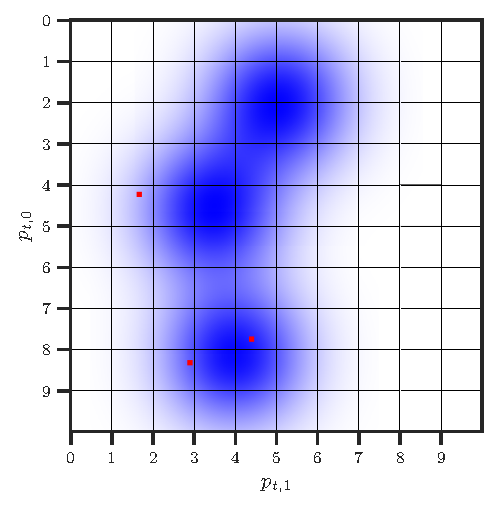
\includegraphics[scale=0.5]{figures/path-scene.pdf}
                \par Environment sample
            \end{figure}
        \end{column}
        \begin{column}{0.5\textwidth}
            \begin{figure}
                \centering
                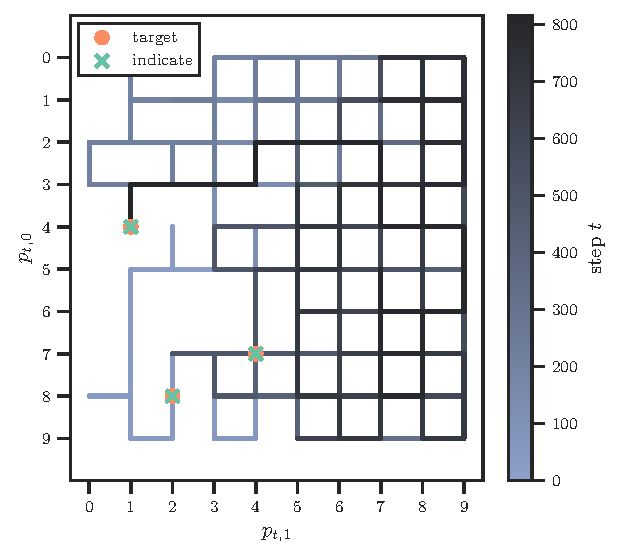
\includegraphics[scale=0.5]{figures/path-random.pdf}
                \par Random baseline
            \end{figure}
        \end{column}
    \end{columns}
\end{frame}

\begin{frame}
    \begin{columns}
        \begin{column}{0.5\textwidth}
            \begin{figure}
                \centering
                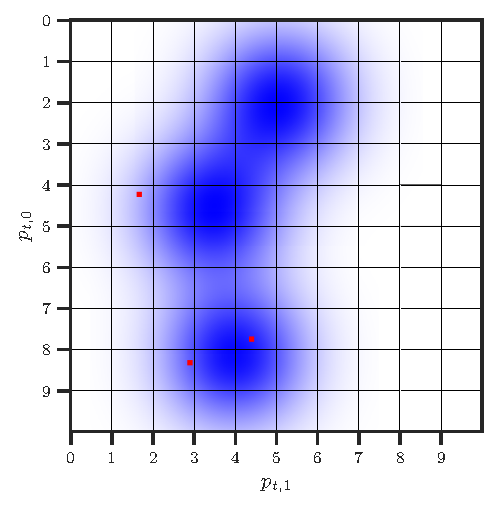
\includegraphics[scale=0.5]{figures/path-scene.pdf}
                \par Environment sample
            \end{figure}
        \end{column}
        \begin{column}{0.5\textwidth}
            \begin{figure}
                \centering
                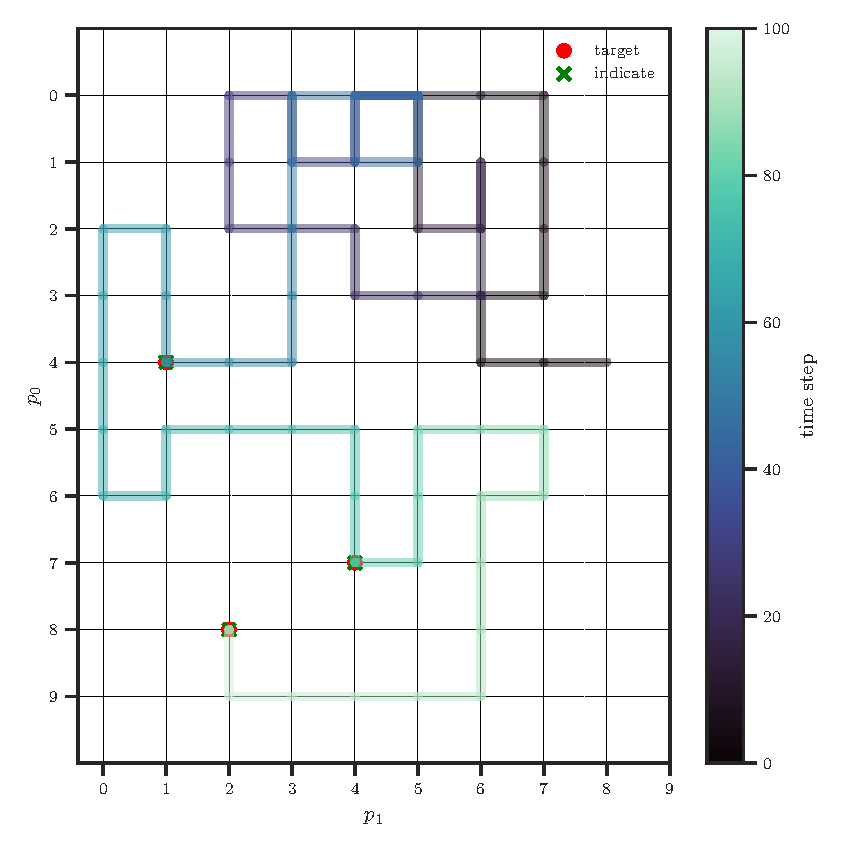
\includegraphics[scale=0.5]{figures/path-greedy.pdf}
                \par Greedy baseline
            \end{figure}
        \end{column}
    \end{columns}
\end{frame}

\begin{frame}
    \begin{columns}
        \begin{column}{0.5\textwidth}
            \begin{figure}
                \centering
                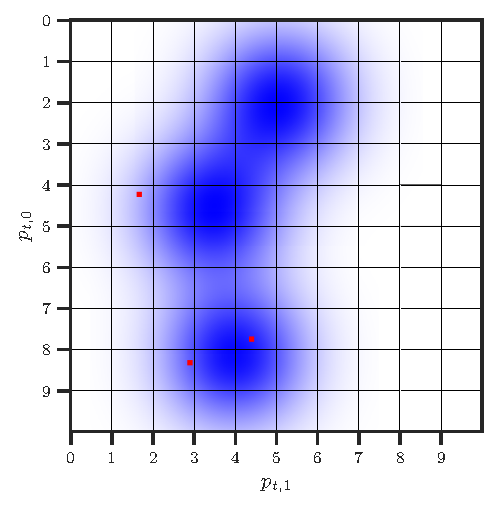
\includegraphics[scale=0.5]{figures/path-scene.pdf}
                \par Environment sample
            \end{figure}
        \end{column}
        \begin{column}{0.5\textwidth}
            \begin{figure}
                \centering
                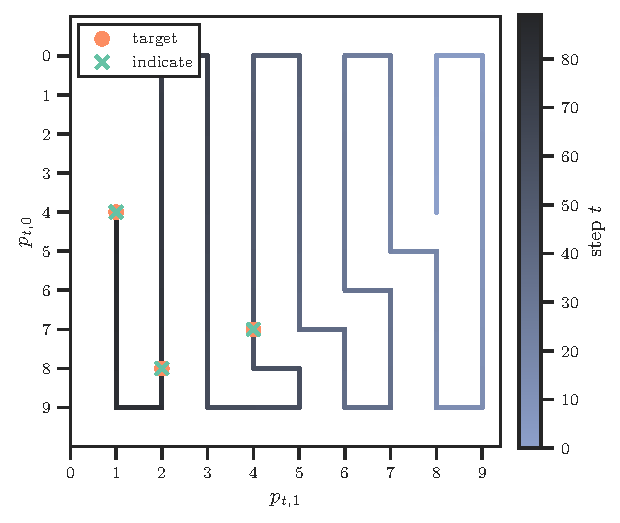
\includegraphics[scale=0.5]{figures/path-exhaustive.pdf}
                \par Exhaustive baseline
            \end{figure}
        \end{column}
    \end{columns}
\end{frame}

\begin{frame}
    \begin{columns}
        \begin{column}{0.5\textwidth}
            \begin{figure}
                \centering
                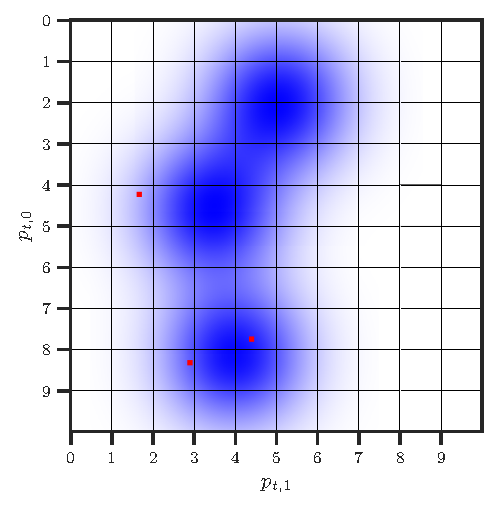
\includegraphics[scale=0.5]{figures/path-scene.pdf}
                \par Environment sample
            \end{figure}
        \end{column}
        \begin{column}{0.5\textwidth}
            \begin{figure}
                \centering
                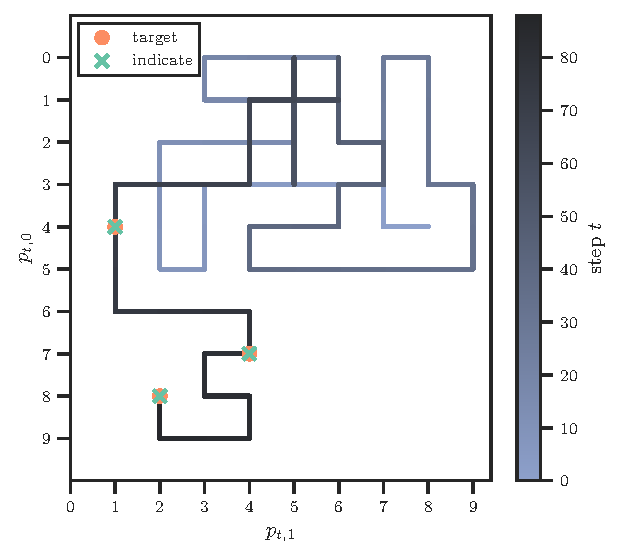
\includegraphics[scale=0.5]{figures/path-handcrafted.pdf}
                \par Handcrafted baseline
            \end{figure}
        \end{column}
    \end{columns}
\end{frame}

\begin{frame}
    \begin{columns}
        \begin{column}{0.5\textwidth}
            \begin{figure}
                \centering
                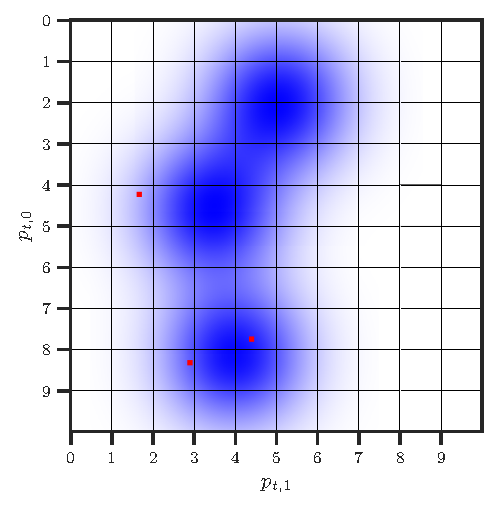
\includegraphics[scale=0.5]{figures/path-scene.pdf}
                \par Environment sample
            \end{figure}
        \end{column}
        \begin{column}{0.5\textwidth}
            \begin{figure}
                \centering
                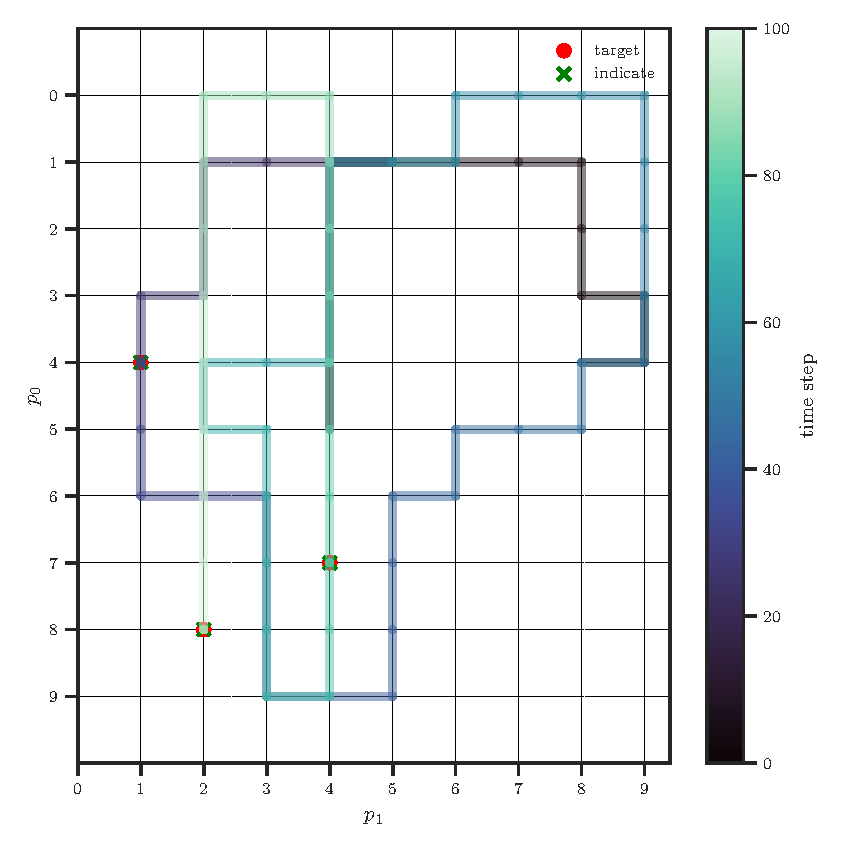
\includegraphics[scale=0.5]{figures/path-lstm.pdf}
                \par Temporal memory
            \end{figure}
        \end{column}
    \end{columns}
\end{frame}

\begin{frame}
    \begin{columns}
        \begin{column}{0.5\textwidth}
            \begin{figure}
                \centering
                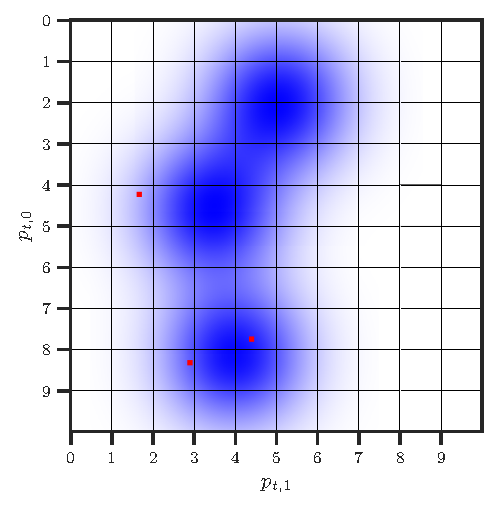
\includegraphics[scale=0.5]{figures/path-scene.pdf}
                \par Environment sample
            \end{figure}
        \end{column}
        \begin{column}{0.5\textwidth}
            \begin{figure}
                \centering
                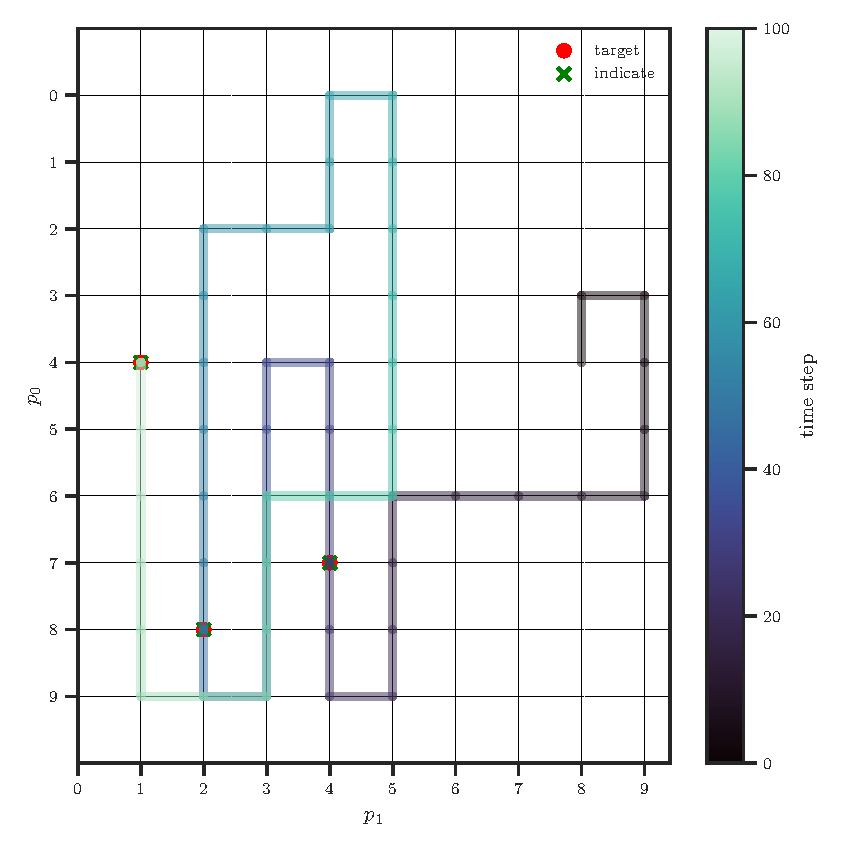
\includegraphics[scale=0.5]{figures/path-map.pdf}
                \par Spatial memory 
            \end{figure}
        \end{column}
    \end{columns}
\end{frame}

\begin{frame}
    \begin{figure}
        \centering
        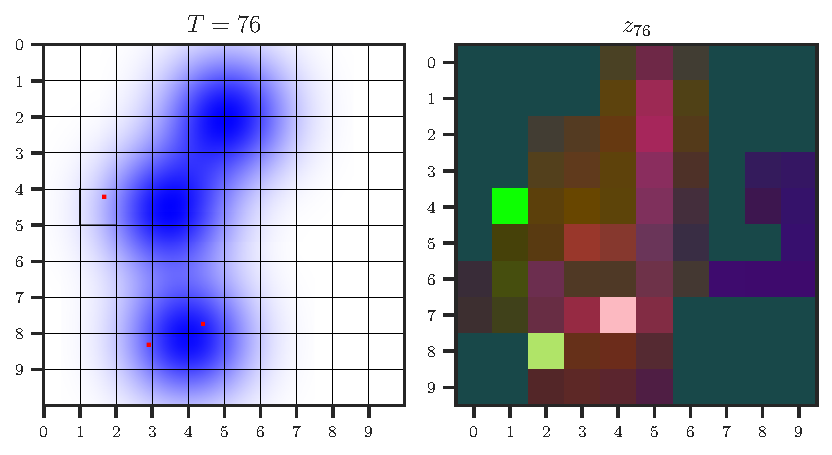
\includegraphics[scale=0.75]{figures/memory-map.pdf}
        \par PCA decomposition of spatial memory after episode.
    \end{figure}
\end{frame}

\begin{frame}
    \begin{table}
        \centering
        Terrain Environment\par\vspace{0.5em}
        \begin{tabular}{lccc}
    \toprule
    Agent & SPL & Success & Length \\
    \midrule
    random & $0.06 \pm 0.01$ & $0.89 \pm 0.04$ & $366.05 \pm 26.96$\\
    greedy & $0.17 \pm 0.01$ & $1.00 \pm 0.00$ & $141.01 \pm 2.31$\\
    exhaustive & $0.22 \pm 0.00$ & $1.00 \pm 0.00$ & $84.11 \pm 0.84$\\
    human & $0.26 \pm 0.02$ & $1.00 \pm 0.00$ & $76.73 \pm 5.33$\\
    \midrule
    temporal & $0.25 \pm 0.02$ & $1.00 \pm 0.01$ & $103.76 \pm 11.69$\\
    spatial & $0.27 \pm 0.01$ & $1.00 \pm 0.00$ & $79.60 \pm 6.88$\\
    \bottomrule
\end{tabular}
    \end{table}

    \begin{center}
        \href{run:./videos/terrain/map/0.mp4}{video 1},
        \href{run:./videos/terrain/map/1.mp4}{video 2},
        \href{run:./videos/terrain/map/2.mp4}{video 3}.
    \end{center}
\end{frame}

\begin{frame}
    \begin{table}
        \centering
        Camera Environment\par\vspace{0.5em}
        \begin{tabular}{lccc}
    \toprule
    Agent & SPL & Success & Length \\
    \midrule
    random & $0.04 \pm 0.00$ & $0.62 \pm 0.03$ & $545.09 \pm 56.25$\\
    greedy & $0.12 \pm 0.01$ & $0.97 \pm 0.01$ & $255.60 \pm 10.44$\\
    exhaustive & $0.37 \pm 0.00$ & $1.00 \pm 0.00$ & $67.03 \pm 0.00$\\
    human & $0.68 \pm 0.08$ & $1.00 \pm 0.00$ & $38.10 \pm 5.72$\\
    \midrule
    temporal & $0.70 \pm 0.02$ & $1.00 \pm 0.00$ & $42.36 \pm 2.05$\\
    spatial & $0.66 \pm 0.03$ & $1.00 \pm 0.00$ & $42.90 \pm 1.73$\\
    \bottomrule
\end{tabular}
    \end{table}

    \begin{center}
        \href{run:./videos/camera/lstm/1.mp4}{video 1},
        \href{run:./videos/camera/lstm/500.mp4}{video 2},
        \href{run:./videos/camera/lstm/1000.mp4}{video 3}.
    \end{center}
\end{frame}

\subsection{Scaling to Larger Search Spaces}

\begin{frame}
    \frametitle{Experiment II: Scaling to Larger Search Spaces}

    \begin{itemize}
        \item Larger search spaces are more difficult.
        \item Stronger demands on memory:
        \begin{itemize}
            \item Remember visited positions.
            \item Remember appearance of environment.
        \end{itemize}
        \item Compare memories on \(10 \times 10\), \(15 \times 15\), and \(20 \times 20\) versions of gaussian environment.
    \end{itemize}
\end{frame}

\begin{frame}
    \begin{figure}
        \centering
        \(10 \times 10\)
        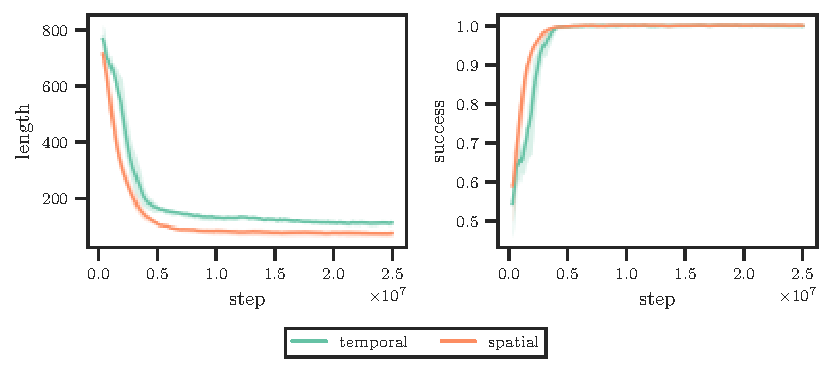
\includegraphics[scale=0.8]{figures/shape-10.pdf}
    \end{figure}
\end{frame}

\begin{frame}
    \begin{figure}
        \centering
        \(15 \times 15\)
        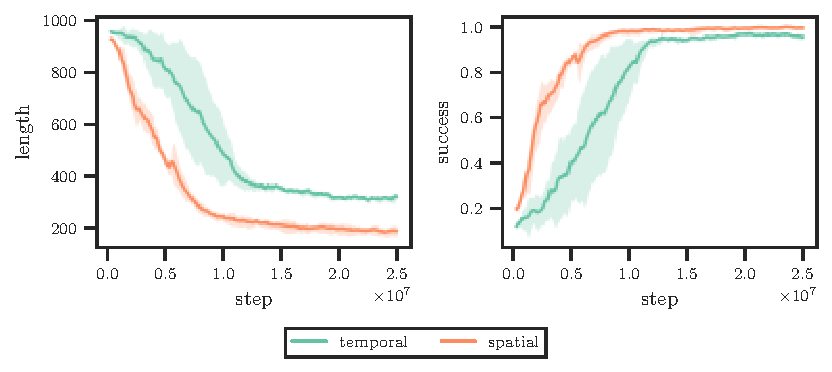
\includegraphics[scale=0.8]{figures/shape-15.pdf}
    \end{figure}
\end{frame}

\begin{frame}
    \begin{figure}
        \centering
        \(20 \times 20\)
        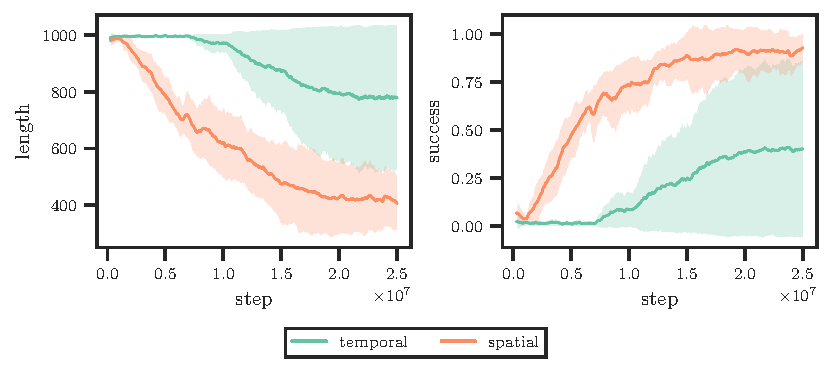
\includegraphics[scale=0.8]{figures/shape-20.pdf}
    \end{figure}
\end{frame}

\subsection{Generalization From Limited Samples}

\begin{frame}
    \frametitle{Experiment III: Generalization From Limited Samples}

    \begin{itemize}
        \item Real-world tasks usually have limited training samples.
        \item Train on 500, 1 000, 5 000 and 10 000 samples of terrain environment.
        \item Test on held out samples from full distribution.
        % high appearance variance and somewhat realistic.
        %Fix seed pool used to generate scenes seen during training.
    \end{itemize}
\end{frame}

\begin{frame}
    \begin{figure}
        \centering
        10000 samples
        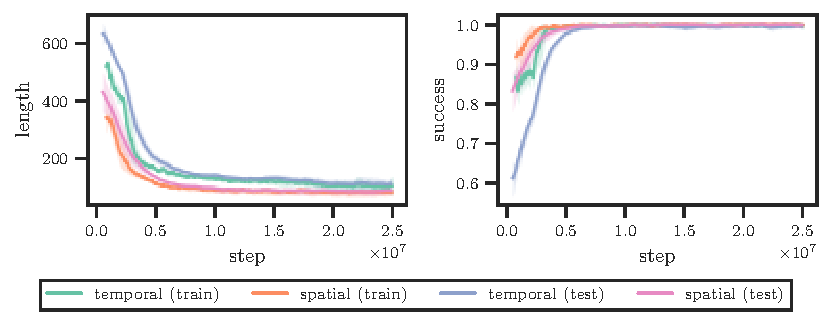
\includegraphics[scale=0.8]{figures/sample-10000.pdf}
    \end{figure}
    % close to full distribution - equal training and test performance for both agents. seemingly no overfitting and good generalization.
\end{frame}

\begin{frame}
    \begin{figure}
        \centering
        5000 samples
        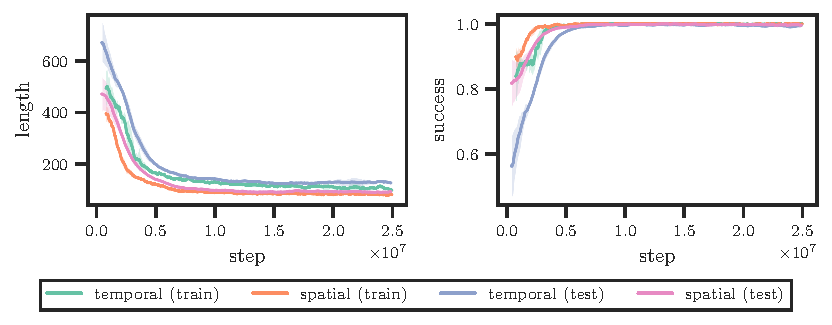
\includegraphics[scale=0.8]{figures/sample-5000.pdf}
    \end{figure}
\end{frame}

\begin{frame}
    \begin{figure}
        \centering
        1000 samples
        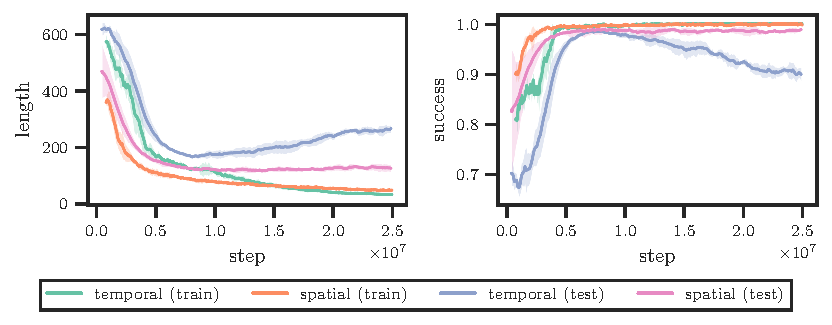
\includegraphics[scale=0.8]{figures/sample-1000.pdf}
    \end{figure}
\end{frame}

\begin{frame}
    \begin{figure}
        \centering
        500 samples
        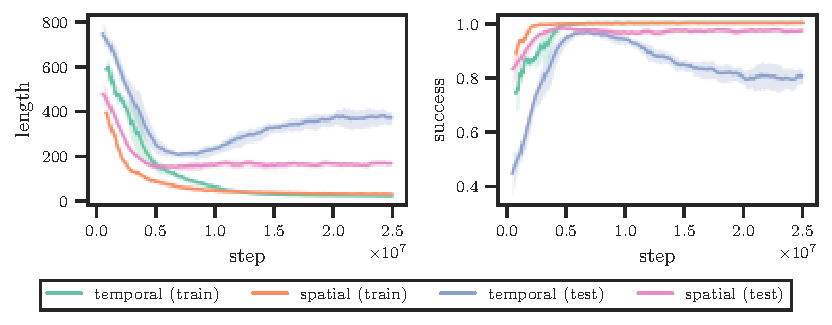
\includegraphics[scale=0.8]{figures/sample-500.pdf}
    \end{figure}
\end{frame}
\chapter{Conclusion}
\label{cha:conclusion}

This chapter contains a summarization of the purpose and the research
questions. To what extent has the aim been achieved, and what are the
answers to the research questions?

The consequences for the target audience (and possibly for researchers
and practitioners) must also be described. There should be a section
on future work where ideas for continued work are described. If the
conclusion chapter contains such a section, the ideas described
therein must be concrete and well thought through.


\section*{References}

\begin{frame}[t,allowframebreaks,noframenumbering]
    \frametitle{References}
    \bibliographystyle{ieeetr}
    \bibliography{references}
\end{frame}

\appendix

\begin{frame}[noframenumbering]
    \frametitle{Implementation}

    \begin{itemize}
        \item OpenAI Gym environment interface.
        \item Custom proximal policy optimization implementation.
        \item PyTorch for models and automatic differentiation.
        \item Intel Core i9-10900X CPU.
        \item NVIDIA GeForce RTX 2080 Ti GPU.
    \end{itemize}
\end{frame}

\begin{frame}[noframenumbering]
    \frametitle{Search Paths I}

    \begin{columns}
        \begin{column}{0.5\textwidth}
            \begin{figure}
                \centering
                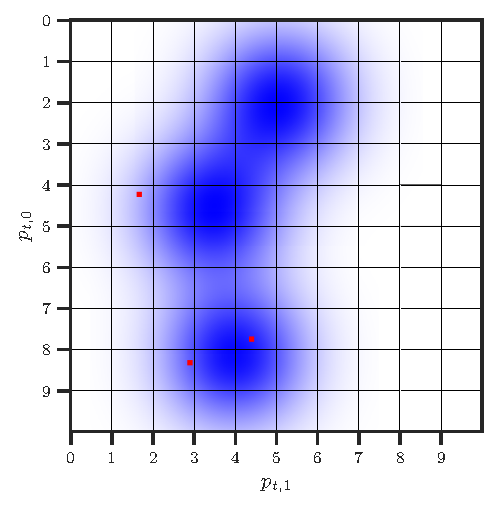
\includegraphics[scale=0.5]{figures/path-scene.pdf}
                \par Environment sample
            \end{figure}
        \end{column}
        \begin{column}{0.5\textwidth}
            \begin{figure}
                \centering
                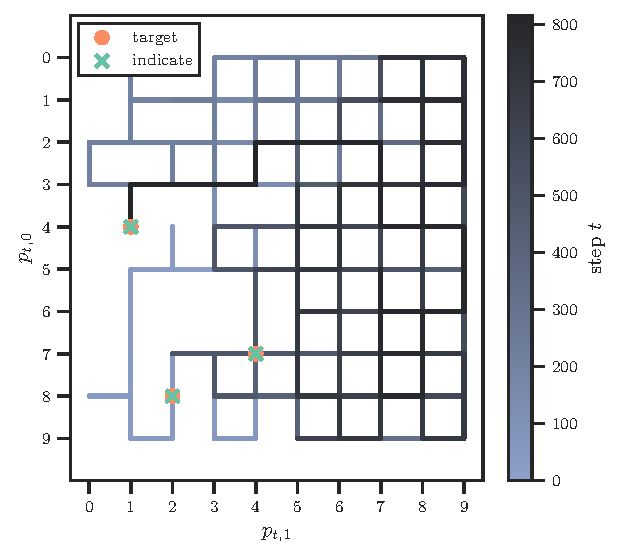
\includegraphics[scale=0.5]{figures/path-random.pdf}
                \par Random baseline
            \end{figure}
        \end{column}
    \end{columns}
\end{frame}

\begin{frame}[noframenumbering]
    \frametitle{Search Paths II}

    \begin{columns}
        \begin{column}{0.5\textwidth}
            \begin{figure}
                \centering
                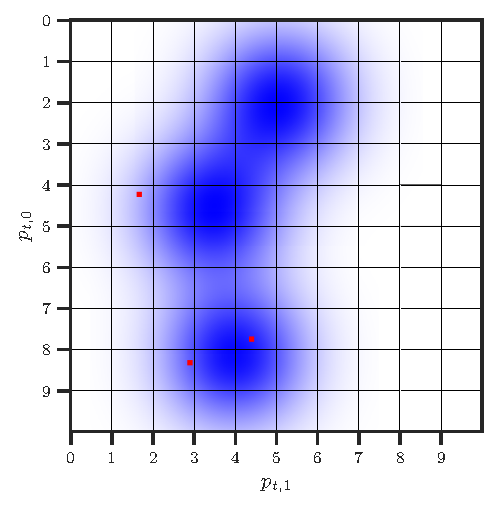
\includegraphics[scale=0.5]{figures/path-scene.pdf}
                \par Environment sample
            \end{figure}
        \end{column}
        \begin{column}{0.5\textwidth}
            \begin{figure}
                \centering
                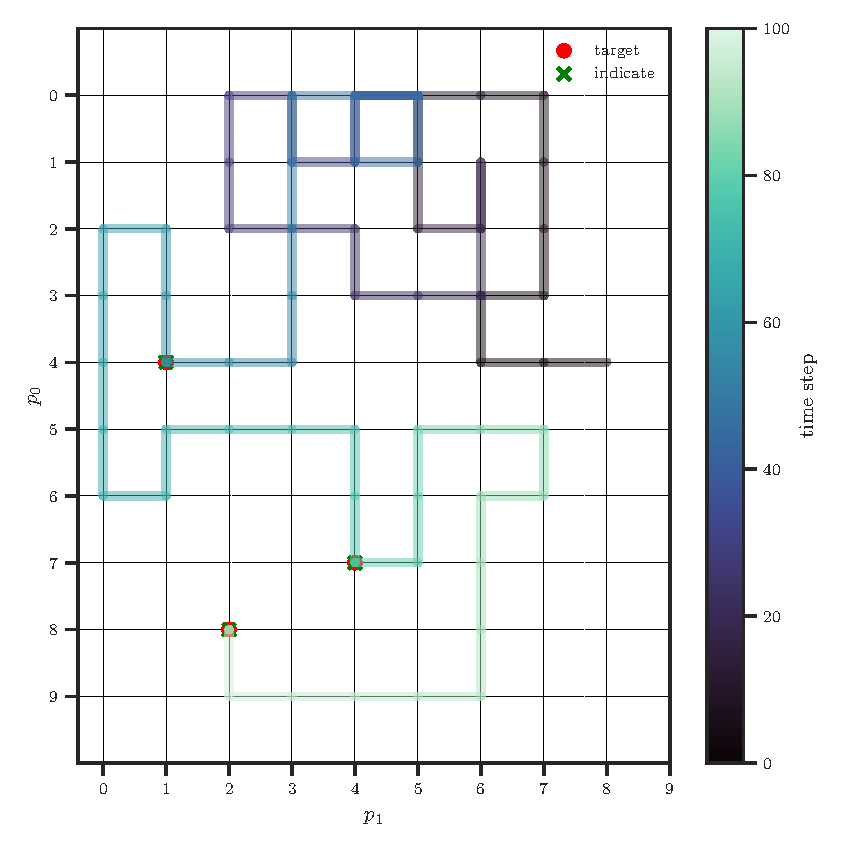
\includegraphics[scale=0.5]{figures/path-greedy.pdf}
                \par Greedy baseline
            \end{figure}
        \end{column}
    \end{columns}
\end{frame}

\begin{frame}[noframenumbering]
    \frametitle{Search Paths III}

    \begin{columns}
        \begin{column}{0.5\textwidth}
            \begin{figure}
                \centering
                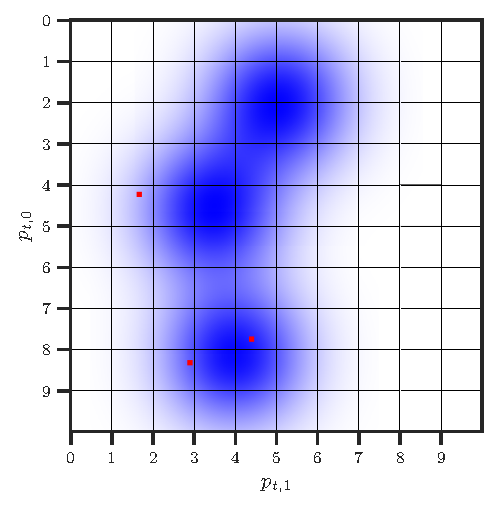
\includegraphics[scale=0.5]{figures/path-scene.pdf}
                \par Environment sample
            \end{figure}
        \end{column}
        \begin{column}{0.5\textwidth}
            \begin{figure}
                \centering
                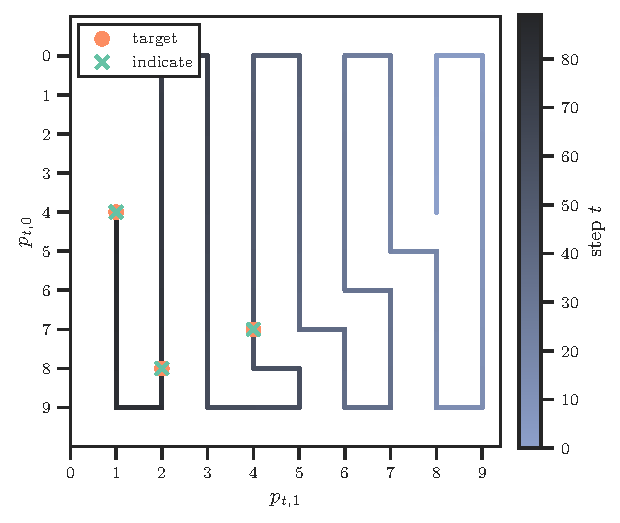
\includegraphics[scale=0.5]{figures/path-exhaustive.pdf}
                \par Exhaustive baseline
            \end{figure}
        \end{column}
    \end{columns}
\end{frame}

\begin{frame}[noframenumbering]
    \frametitle{Search Paths IV}

    \begin{columns}
        \begin{column}{0.5\textwidth}
            \begin{figure}
                \centering
                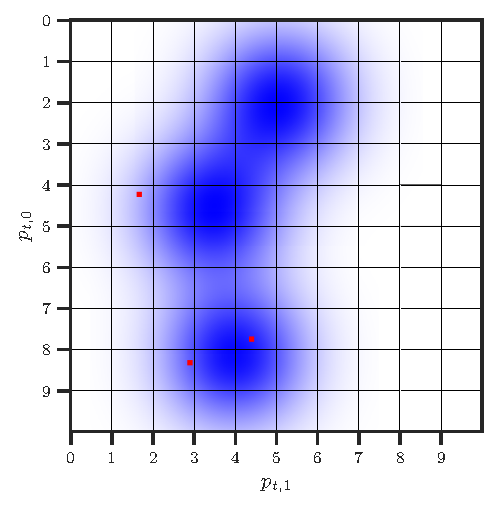
\includegraphics[scale=0.5]{figures/path-scene.pdf}
                \par Environment sample
            \end{figure}
        \end{column}
        \begin{column}{0.5\textwidth}
            \begin{figure}
                \centering
                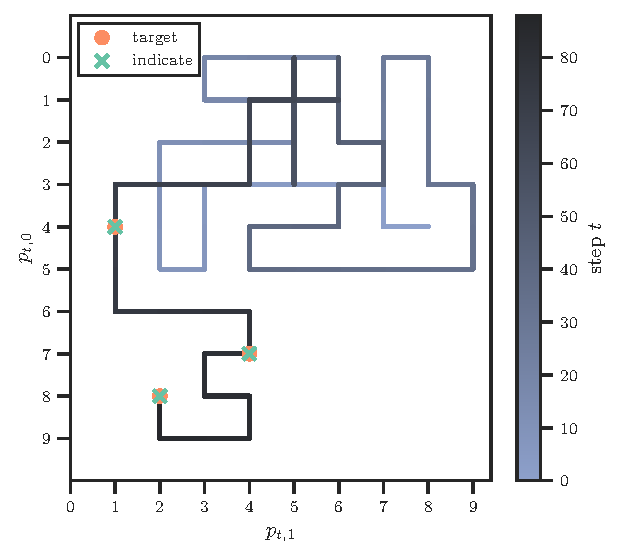
\includegraphics[scale=0.5]{figures/path-handcrafted.pdf}
                \par Handcrafted baseline
            \end{figure}
        \end{column}
    \end{columns}
\end{frame}

\begin{frame}[noframenumbering]
    \frametitle{Search Paths V}

    \begin{columns}
        \begin{column}{0.5\textwidth}
            \begin{figure}
                \centering
                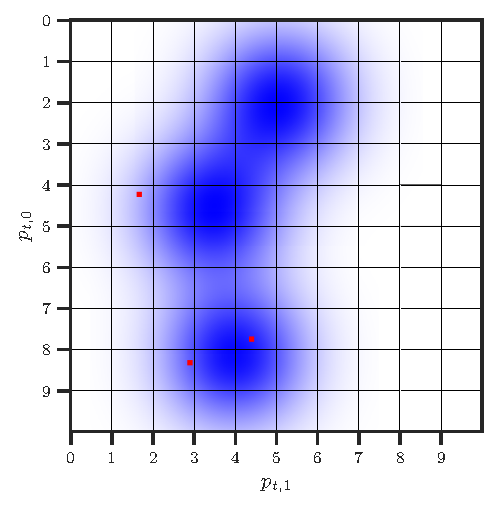
\includegraphics[scale=0.5]{figures/path-scene.pdf}
                \par Environment sample
            \end{figure}
        \end{column}
        \begin{column}{0.5\textwidth}
            \begin{figure}
                \centering
                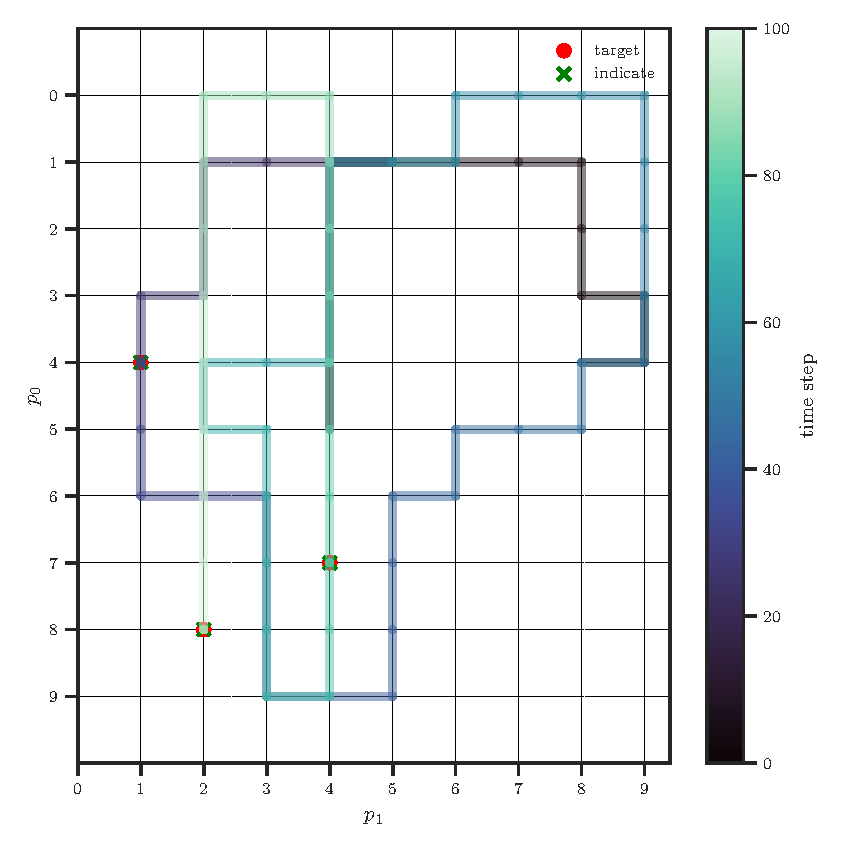
\includegraphics[scale=0.5]{figures/path-lstm.pdf}
                \par Temporal memory
            \end{figure}
        \end{column}
    \end{columns}
\end{frame}

\begin{frame}[noframenumbering]
    \frametitle{Search Paths VI}

    \begin{columns}
        \begin{column}{0.5\textwidth}
            \begin{figure}
                \centering
                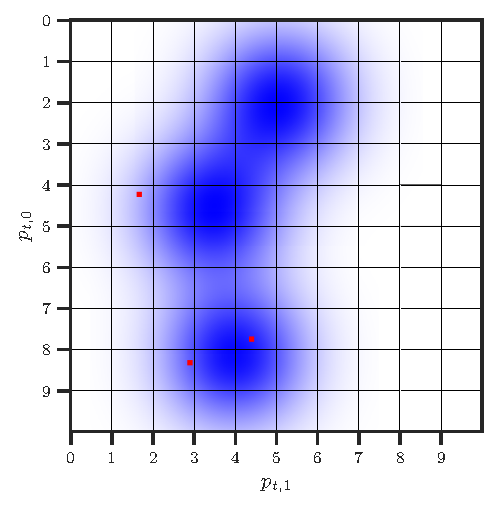
\includegraphics[scale=0.5]{figures/path-scene.pdf}
                \par Environment sample
            \end{figure}
        \end{column}
        \begin{column}{0.5\textwidth}
            \begin{figure}
                \centering
                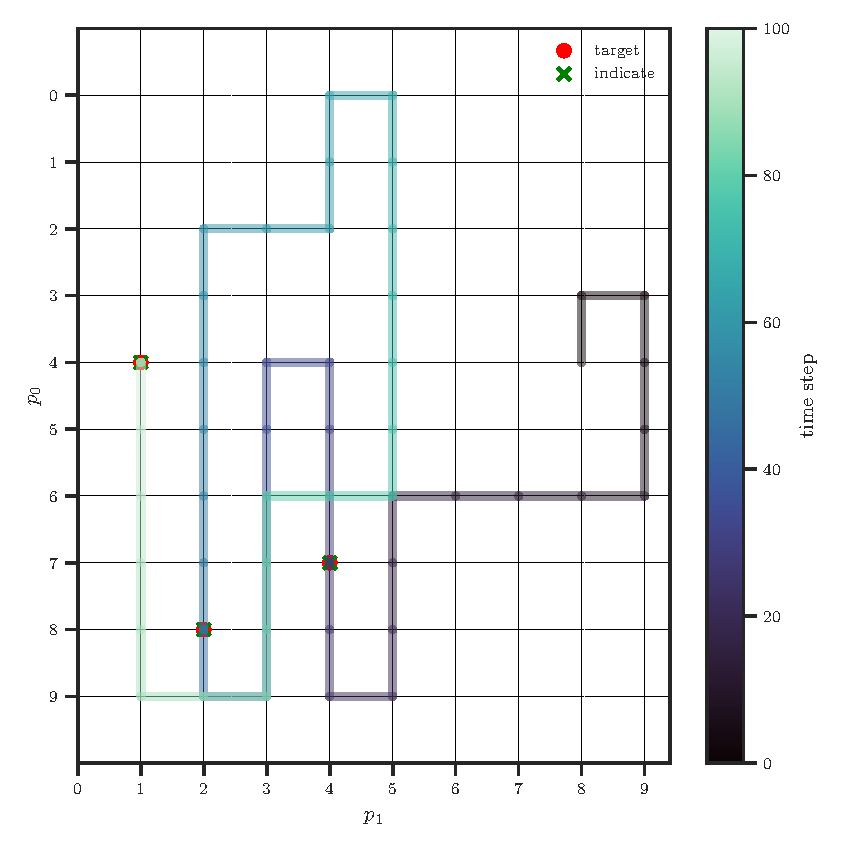
\includegraphics[scale=0.5]{figures/path-map.pdf}
                \par Spatial memory 
            \end{figure}
        \end{column}
    \end{columns}
\end{frame}

\begin{frame}[noframenumbering]
    \frametitle{Memory Viualization}

    \begin{figure}
        \centering
        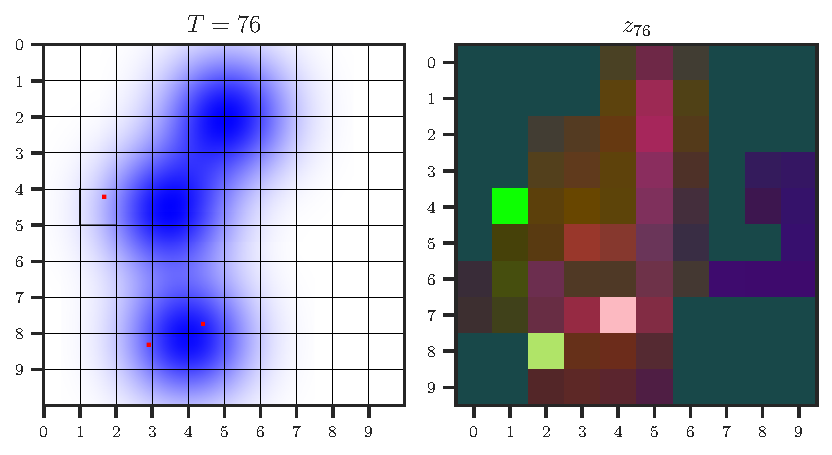
\includegraphics[scale=0.75]{figures/memory-map.pdf}
        \par PCA decomposition of spatial memory after episode.
    \end{figure}
\end{frame}


\end{document}